\documentclass[12pt,a4paper,twoside,openright]{book}

%%%%%%%%%%%%%%%%%%%%%%%%%%%%%%%%%%%%%%%%%%%%%%%%%%%%%%%%%%%%%%%%%%%%
%  Template per Tesi di Laurea                                     %
%                                                                  %
%%%%%%%%%%%%%%%%%%%%%%%%%%%%%%%%%%%%%%%%%%%%%%%%%%%%%%%%%%%%%%%%%%%%

               %%%%%%%%%%%%%%%%%%%%%%%%%%%%%%%%%%%%%%
               %    Scelta dei package da usare     %
               %%%%%%%%%%%%%%%%%%%%%%%%%%%%%%%%%%%%%%
\usepackage{macros}


               %%%%%%%%%%%%%%%%%%%%%%%%%%%%%%%%%%%%%%
               %  Scelta del tipo di font da usare  %
               %%%%%%%%%%%%%%%%%%%%%%%%%%%%%%%%%%%%%%

%\usepackage{times,mathptm}
%\usepackage{palatino,mathpple}
%\usepackage{bookman}
%\usepackage{newcent}

               %%%%%%%%%%%%%%%%%%%%%%%%%%%%%%%%%%%%%%%%
               % Scelta delle dimensioni della pagina %
               %%%%%%%%%%%%%%%%%%%%%%%%%%%%%%%%%%%%%%%%

\setlength{\textwidth}{16.0cm}
\setlength{\textheight}{21cm}
\setlength{\footskip}{3cm}



               %%%%%%%%%%%%%%%%%%%%%%%%%%%%%%%%%%%%%%
               %  Informazioni generali sulla Tesi  %
               %    da usare nell'intestazione      %
               %%%%%%%%%%%%%%%%%%%%%%%%%%%%%%%%%%%%%%

\titolo{Engineering complex computational ecosystems}
\candidato{Danilo Pianini}
\annoaccademico{2015}
\facolta{Ingegneria}
\dipartimento{DEIS - Dipartimento di Elettronica, Informatica e Sistemistica}
\dottorato{PhD Course in Electronics, Computer Science and Telecommunications}
\settoreconcorsuale{09/H1}
\settoredisciplinare{ING-INF/05}
\ciclo{XXVII}
\tutor{Antonio Natali}
\relatore{Mirko Viroli}
% \correlatoreb{Andrea Roli}
% \correlatorec{Mirko Viroli}
\coordinatore{Alessandro Vanelli Coralli}
\dedica{
\emph{\mbox{~~~~~~~~~~~~~~~~~~~~~~~~~~~~~~~~~~~~~~~}Lorem ipsum dolor sit amet. \\
%
\mbox{~~~~~~~~~~~~~~~~~~~~~~~~~~~~~~~~~~~~~~~~~~~~}consectetur adipiscing elit.\\
%
\mbox{~~~~~~~~~~~~~~~~~~~~~~~~~~~~~~~~~~~~~~~~~~~~}Sed fringilla quis mauris id sagittis everything.}\\ \\ \\ \\
\noindent \emph{\textbf{Acknowledgements}}\\ \\
Curabitur commodo dictum risus laoreet tincidunt. Sed dapibus nec ex sit amet consequat. Quisque cursus est sit amet lectus tempor, nec egestas sapien rutrum. Sed dapibus consequat egestas. Quisque blandit, tellus et molestie interdum, augue est molestie lorem, tristique congue metus massa sed eros. Vivamus fermentum erat a faucibus porta. Praesent sit amet risus leo. Integer venenatis lectus sed euismod euismod. Ut pulvinar fermentum sagittis. Aliquam maximus nisl velit, ac varius tellus dignissim in. Fusce nibh dolor, blandit vel nisl non, vehicula tincidunt lorem. Suspendisse fringilla magna ac justo fermentum, nec accumsan odio sollicitudin. Maecenas consectetur, nulla sit amet ultricies pretium, metus sapien posuere turpis, in lobortis tellus turpis ac ipsum. Aliquam sollicitudin augue a aliquam volutpat. Mauris bibendum nunc id est ullamcorper, nec feugiat elit dapibus.\\
%
Duis tincidunt maximus justo, id convallis mauris mattis congue. Maecenas ullamcorper laoreet lacinia. Praesent luctus dictum metus, sed ultrices dui. Fusce fringilla eu est sit amet porta. Aliquam ornare eleifend congue. Aliquam orci urna, accumsan nec metus a, tincidunt pulvinar augue. Nunc eu vulputate lectus. Morbi placerat varius purus at scelerisque. Mauris malesuada ut massa non porta. Quisque ac efficitur odio. Aliquam scelerisque dapibus felis in ullamcorper. Pellentesque ullamcorper massa quis nibh suscipit elementum. Suspendisse tincidunt, sem non porta consectetur, arcu mauris mollis mi, ut commodo libero diam ut risus.
}
\data{March 2015}
\signature{\emph{Danilo Pianini}}

              %%%%%%%%%%%%%%%%%%%%%%%%%%%%%%%%%%%%%%
               % Fine Preambolo                     %
               % Inizio tesi                        %
               %%%%%%%%%%%%%%%%%%%%%%%%%%%%%%%%%%%%%%

\begin{document}

%%%%%%%%%%%%%%%%%%%%%%%%%
% inizio prefazione
%
% pagina del titolo, indice, sommario
%%%%%%%%%%%%%%%%%%%%%%%%%
\frontmatter
\maketitle
\pagestyle{plain}
\tableofcontents

\chapter*{\centering Abstract}
\addcontentsline{toc}{chapter}{Abstract}

This work presents advancements of the latest three years in the engineering techniques for self-organising pervasive ecosystems of devices and services.
%
The inherent complexity of such systems poses new challenges to those who try to dominate the complexity by applying the principles of engineering.

The recent growth in number and distribution of devices with decent computational and communicational abilities, that got suddenly accelerated with the massive diffusion of smartphones and tablets, is envisioning a world with a much higher density of devices in space.
%
This already high device density is probably going to consistently rise if the diffusion of wearable devices gets momentum.
%
Also, communication technologies seem to be focussing on short-range device-to-device (P2P) interactions, with technologies such as \btle{} and Near-Field Communication getting more and more diffused.

Locality and situatedness become key to provide the best possible experience to users, and the classic model of a centralised, enormously powerful server gathering data and processing it is likely to get less and less efficient with device density.
%
Accomplishing complex global tasks without a centralised controller responsible of aggregating data from devices, however, still is a challenging task.
%
In particular, it is hard to understand which device-local programs could properly interact and guarantee a certain global service level.
%
Such local-to-global issue makes the application of engineering principles challenging at least.

In this work, I lay the foundations of my contribution by first analysing the state of the art in coordination systems, namely in those software frameworks devoted to control and promote interactions among independent software entities.
%
I then motivate my work, by describing the main issues of pre-existing tools and practices and identifying the improvements that would benefit the design of such complex software ecosystems.
%
My contribution is described in \Cref{contribution}, and can be divided in three main branches: i) a novel simulation tool for pervasive ecosystems, ii) introduction of novel and improvements over existing self-organisation patterns, iii) the creation of a new language and interpreter based on ``field calculus'' and its integration with the previously mentioned simulator.
%
Finally, I draw conclusions and future works.

\mainmatter

% stile della pagina
\pagestyle{fancy}
\fancyhead[LE,RO]{\bfseries\thepage}

\part{Background and Motivation}
\label{background}
\chapter{Pervasive computing}
\label{pervasive-devices}

It is no mystery that, with the huge progresses of miniaturisation, computational-capable devices are populating the world.
%
The diffusion got momentum with affordable ``personal computers'' that made their way in a one-device-per-family world.
%
Laptops boosted the process, offering user a personal and mobile device.

The pervasive revolution, however took place when the phones became ``smart'', and with the subsequent improvements in the communication technologies.
%
In this chapter, I try to briefly walk the path of success of personal mobile devices, describing also the probable newcomer, namely the wearable devices.
%
I also focus on the current status of the communication protocols, their range and usage, and I try to foresee which world are we going to build if the current trend continues.

\section{Smart, portable devices}

\begin{figure}
	\centering
	
\includegraphics[width=0.99\textwidth]{img/iphone}
	\caption{Apple iPhone is one of the first devices without any physical keyboard, and the first smartphone to gain worldwide success. \emph{Source: Wikimedia.}}
	\label{img:iphone}
\end{figure}

When Apple in 2007 released the first iPhone (\Cref{img:iphone}), a mobile revolution started.
%
Even though other manufacturers proposed products similar to iPhone under the point of view of communication technologies and computational capabilities in the same time frame (e.g. Nokia N810), the Apple's smartphone was the first gaining widespread adoption.
%
It is not really relevant for this work to understand if the branding, the design, the multi-touch finger based interaction UI or the feature set was the key of its commercial success: what really matters is that, starting 2007, every person began to carry with her a personal device featuring both the abilities to communicate and compute.
%
The reason, besides the success of iPhone in the higher segment of the phone market, is mainly to attribute to the widespread diffusion of similar but cheaper and less powerful devices in the lower segments.
%
This kind of devices ultimately pushed the market share of the dominating today's mobile operating system, Google's Android.

This trend towards a higher diffusion got another leap forward three years later, in 2010, when a device with a feature set similar to iPhone, but with no phone abilities  and a bigger screen was released: the iPad.
%
As iPhone gave new vitality and perspectives to the phone arena, iPad revitalised a market that was languishing: the tablets.
%
Tablet devices as they were conceived before iPad launched were nothing more than small laptops with a screen that could be rotated or detached from the keyboard, and a touch-screen normally used with the help of a pen.
%
They changed from devices designed for a professional niche to widespread tools, up to the point that Gartner forecasts their shipments to overtake in 2015 those of desktop PC and laptops aggregated \footnote{\url{http://www.gartner.com/newsroom/id/2791017}}.

The new frontier of pervasive is probably the wearable technology. Smartphones were precursors, they substituted mobile phones introducing new features and they have potential to substitute our wallets (see, for instance, payments through NFC technology) and keys, becoming the only object we need to carry with us in our pockets.
%
Still there are other accessories which are hard to replace, above all watches and glasses.
%
Yes, smartphone can easily show the current time accurately (and, to be honest, also feature phones had this feature well before 2007), but they require the user to pick them from the pocket, turn them on, and sometimes, depending on privacy settings, also unlock them.
%
The whole operation, takes a much longer time and higher effort with respect to just rotating a wrist.
%
This might be the reason why, despite the explosive expansion of smartphones, the wristwatches market did not declined, as an analysis from MarketWatch points out \footnote{\url{http://www.marketwatch.com/story/the-watchs-time-isnt-up-2013-07-01}}.

\begin{figure}
	\centering
	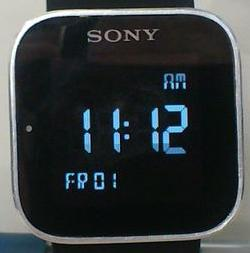
\includegraphics[height=5cm]{img/sony-sw}
	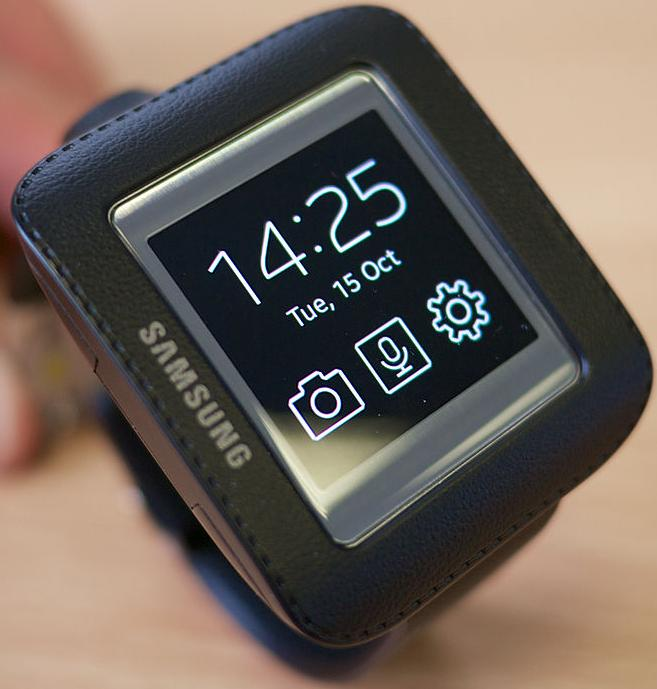
\includegraphics[height=5cm]{img/samsung-gg}
	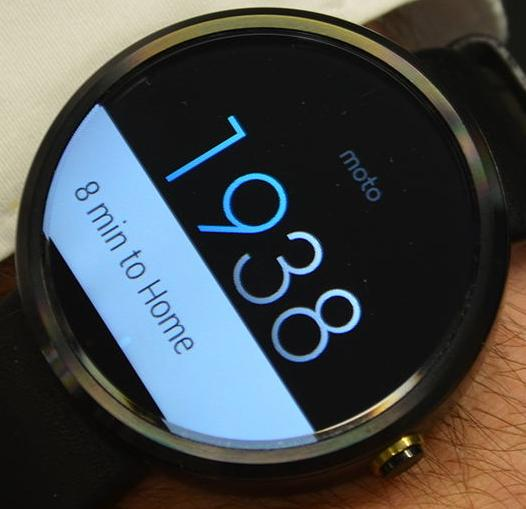
\includegraphics[height=5cm]{img/moto360}
	\caption{Smart watches. From left to right: Sony Smartwatch \emph{(Source: Alex S.H. Lin)}, Samsung Galaxy Gear \emph{(Source: Karlis Dambrans)}, Motorola Moto 360.}
	\label{img:watches}
\end{figure}

There is room for manufacturers to create new portable devices.
%
Sony, starting 2012, has produced a series of smartwatches, such as those in \Cref{img:watches} that pair with a smartphone and provide quick access to some of its functionalities.
%
The success of such solution is not huge, but despite that many other companies are interested in this market: Samsung, Motorola and Apple presented devices meant to replace the classic wristwatch, a clear sign that this market is in expansion.
%
At the time of writing, the main issues that slow the widespread adoption of such solutions are battery duration and dependence on a smartphone.

\begin{figure}
	\centering
	
\includegraphics[width=0.99\textwidth]{img/gglass}
	\caption{Google Glass. In this image, it is possible to see both the camera (on the left hand side) and the semi-transparent head-mounted display. Are those devices going to be part of our everyday life? \emph{Source: Wikimedia.}}
	\label{img:gglass}
\end{figure}

Another notable attempt to make a common accessory smarter is Google Glass project, depicted in \Cref{img:gglass}.
%
Their goal is to enhance the experience of wearing glasses by attaching a device with a camera, an optical head-mounted display, and the abilities to locate itself and communicate with other devices.
%
Google Glass, at the time of writing, are way to expensive (with the kit sold at \$1500) for being able to penetrate the general public, but they are an interesting anticipation of possible future devices.

On the same line of such wearable devices, a discrete success is being achieved by the so called ``fit bands''.
%
They are bracelets equipped with low energy sensors, mainly accelerometers and gyroscopes, which are used to keep track of user's activity.
%
Depending on the model, they can be used to monitor some user's health parameters, such as the number of steps walked per day or heartbeats.
%
They normally work along with another device, a smartphone or a tablet.
%
Such devices, due to their precise market niche and reasonably low price (the Chinese manufacturer Xiaomi recently introduced a low-end wristband at around \$15) are having a notable success.

The wearable devices segment also includes less common devices such as ``smart shoes'' and materials that can be used to make clothing, such as e-textiles.
%
It is a market in expansion, greatly beneficing from recent increases in performance per watt efficiency.
%
If the trend continues, it is likely that we will more and more powerful wearable devices on sale at cheaper and cheaper prices, and a consequent widespread diffusion.
%
The same sort may occur to other parts of our life: kitchen gear, indoor lights and many other objects are getting more and more ``smart'' around us.
%
We may, literally, end up with a world where every single object embeds computational and communicational abilities.

A problem arise: how can software engineers deal with such a complexity?

\section{Communication technologies}

Besides miniaturisation, and as a consequence the increase of computational density in space, another factor played a fundamental role in the world of pervasive computing: the ability to communicate, and in particular the ability to rely on wireless communication, which is of paramount importance when considering mobility.

In later years, many communication means arose.
%
They largely differ in terms of range, protocols, and availability.
%
In this section, I try to resume the most diffused technologies available on today's devices, but the reader is warned: keep in mind that such technologies are evolving very quickly, and the scenario is incredibly fluid.

\subsection{International Mobile Telecommunications}
\label{International Mobile Telecommunications}

This first mean of communication is designed to allow mobile devices to access the Internet from anywhere in the world, relying on the existing mobile phone infrastructure.
%
Such technologies are meant to be used with the standard IP protocols, and they are normally used to get access to public services, in particular to the world wide web.
%
They are not designed for a local peer-to-peer (P2P) communication, and as a consequence they provide no mean to exploit locality.
%
The diffusion of such communication protocols is widespread, in particular among smartphones.
%
Due to the fact that they rely on the mobile phone network, they require a contract with a mobile telecommunications provider, and as such they are much less diffused in tablets and other portable devices.

\begin{figure}
	\centering
	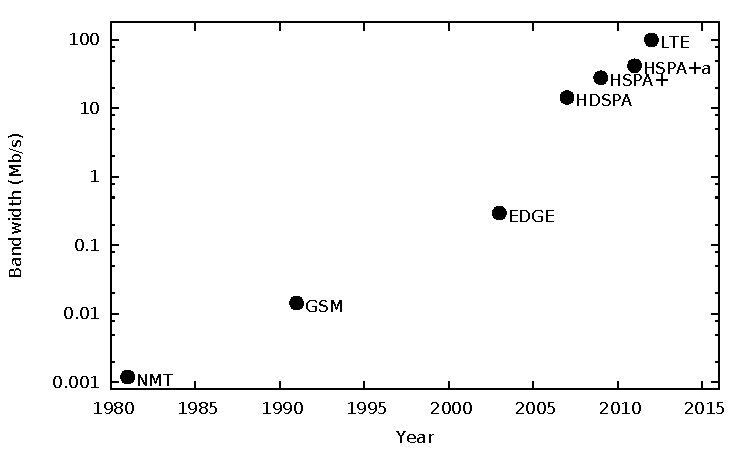
\includegraphics[width=0.99\textwidth]{img/charts/mobile-data-performance}
	\caption{
		Maximum download bandwidth available for mobile devices with time.
		%
		Each point is labelled with the specific communication technology name.
		%
		For the most recent multiple-input-multiple-output (MIMO) technologies, such as LTE, a conservative single input channel was used.
	}
	\label{img:mobile-bandwidth}
\end{figure}

The possibility of accessing the Internet from everywhere is probably one of the key bricks that allowed for the huge success of smartphones in today's world.
%
As \Cref{img:mobile-bandwidth} shows, the bandwidth available grew exponentially with time, to the point that in some countries (e.g. in Italy, at the time of writing) the best available mobile connections offer a higher performance than the best available home connection
%
\footnote{At the time of writing, Telecom Italia Mobile offers mobile connections on LTE with a download bandwidth up to 225Mb/s.
%
Fastweb, the company offering the faster solutions for fiber-to-home connections, goes up to 100Mb/s.}.
%
Such performance unlock the possibility of fully exploiting the possibilities of the world wide web, including cloud services and fruition of multimedia content.

If bandwidth is not currently an issue for international mobile telecommunications, the situation is well different when it comes to device density.
%
Any of us probably experienced network availability issues when participating crowded events, such as concerts or sport events.
%
The current technology, in fact, makes all the network user share the same physical resources: when the device density is too high, there is simply not enough space in the frequency spectrum to grant a decent bandwidth to everyone.
%
Future networks (5G, and presumably those that will follow) are focussing toward this issue among others \cite{5g}.
%
In particular, a so-called ``spectrum crunch'' is expected due to the expected traffic increase (thousand fold over this decade and still growing into the next), that could not be faced simply with the foreseen steady increase of the spectrum allocated for mobile communication, and will require technological advances \cite{spectrum-crunch}.

\subsection{WiFi}

WiFi technology is the most diffused technology for wireless local networking.
%
It is widely diffused, integrated in all smartphones and tablets and also in other devices, such as printers, gaming consoles and TVs.
%
WiFi devices communicate on a distance that ranges from 20 to 100 meters, depending on the condition of the wireless medium and on the power of the communication devices.
%
The communication speed between two linked devices ranges from 56Mb/s to 300Mb/s.

WiFi was designed to provide wireless access to a local area network.
%
In the most classic ``infrastructure mode'', wireless devices get connected to a so called access point, which is responsible to route packets among wireless devices and bridge the wireless local area network to the wired backbone.
%
Multiple access point that share the network name (SSID) may be connected using wired network technologies, and they will appear as a single, bigger access point.
%
It is also possible to drop the wired backbone, but specific access points are required.

Also, some WiFi devices provided ``ad-hoc mode'', allowing multiple devices to directly communicate without an intermediate access point.
%
This working mode was problematic, mainly due to the fact a standard communication protocol for peer-to-peer WiFi communication was missing.
%
This lack was filled with WiFi Direct, which provides a protocol by which one of the devices that want to communicate directly becomes the access point, allowing for direct communication.
%
The most common usage of such a feature are direct file sharing between devices and connection to peripheral devices such as printers or scanners.

\subsection{Bluetooth and Bluetooth LE}

Bluetooth is a technology designed for building energy efficient personal area networks (PANs).
%
Bluetooth devices are assigned a class which identifies the maximum permitted power and, consequently, the maximum operating range.
%
For the most powerful (and power hungry) devices the communication range can go up to 100m.
%
The communication speed ranges from 1Mb/s of the earliest 1.0 version to the 24 Mb/s of version 3.0 and later.

The most interesting features of Bluetooth are not the bandwidth nor the range (WiFi performs better on both), but rather the simple association process and the low power consumption.
%
Thanks to those features Bluetooth found widespread diffusion as a mean to connect low consumption peripherals, such as headsets.
%
Also, it is diffused in cars, and allows user to use the car's audio system as a speakerphone for making calls or listen to music.

\begin{figure}
	\centering
	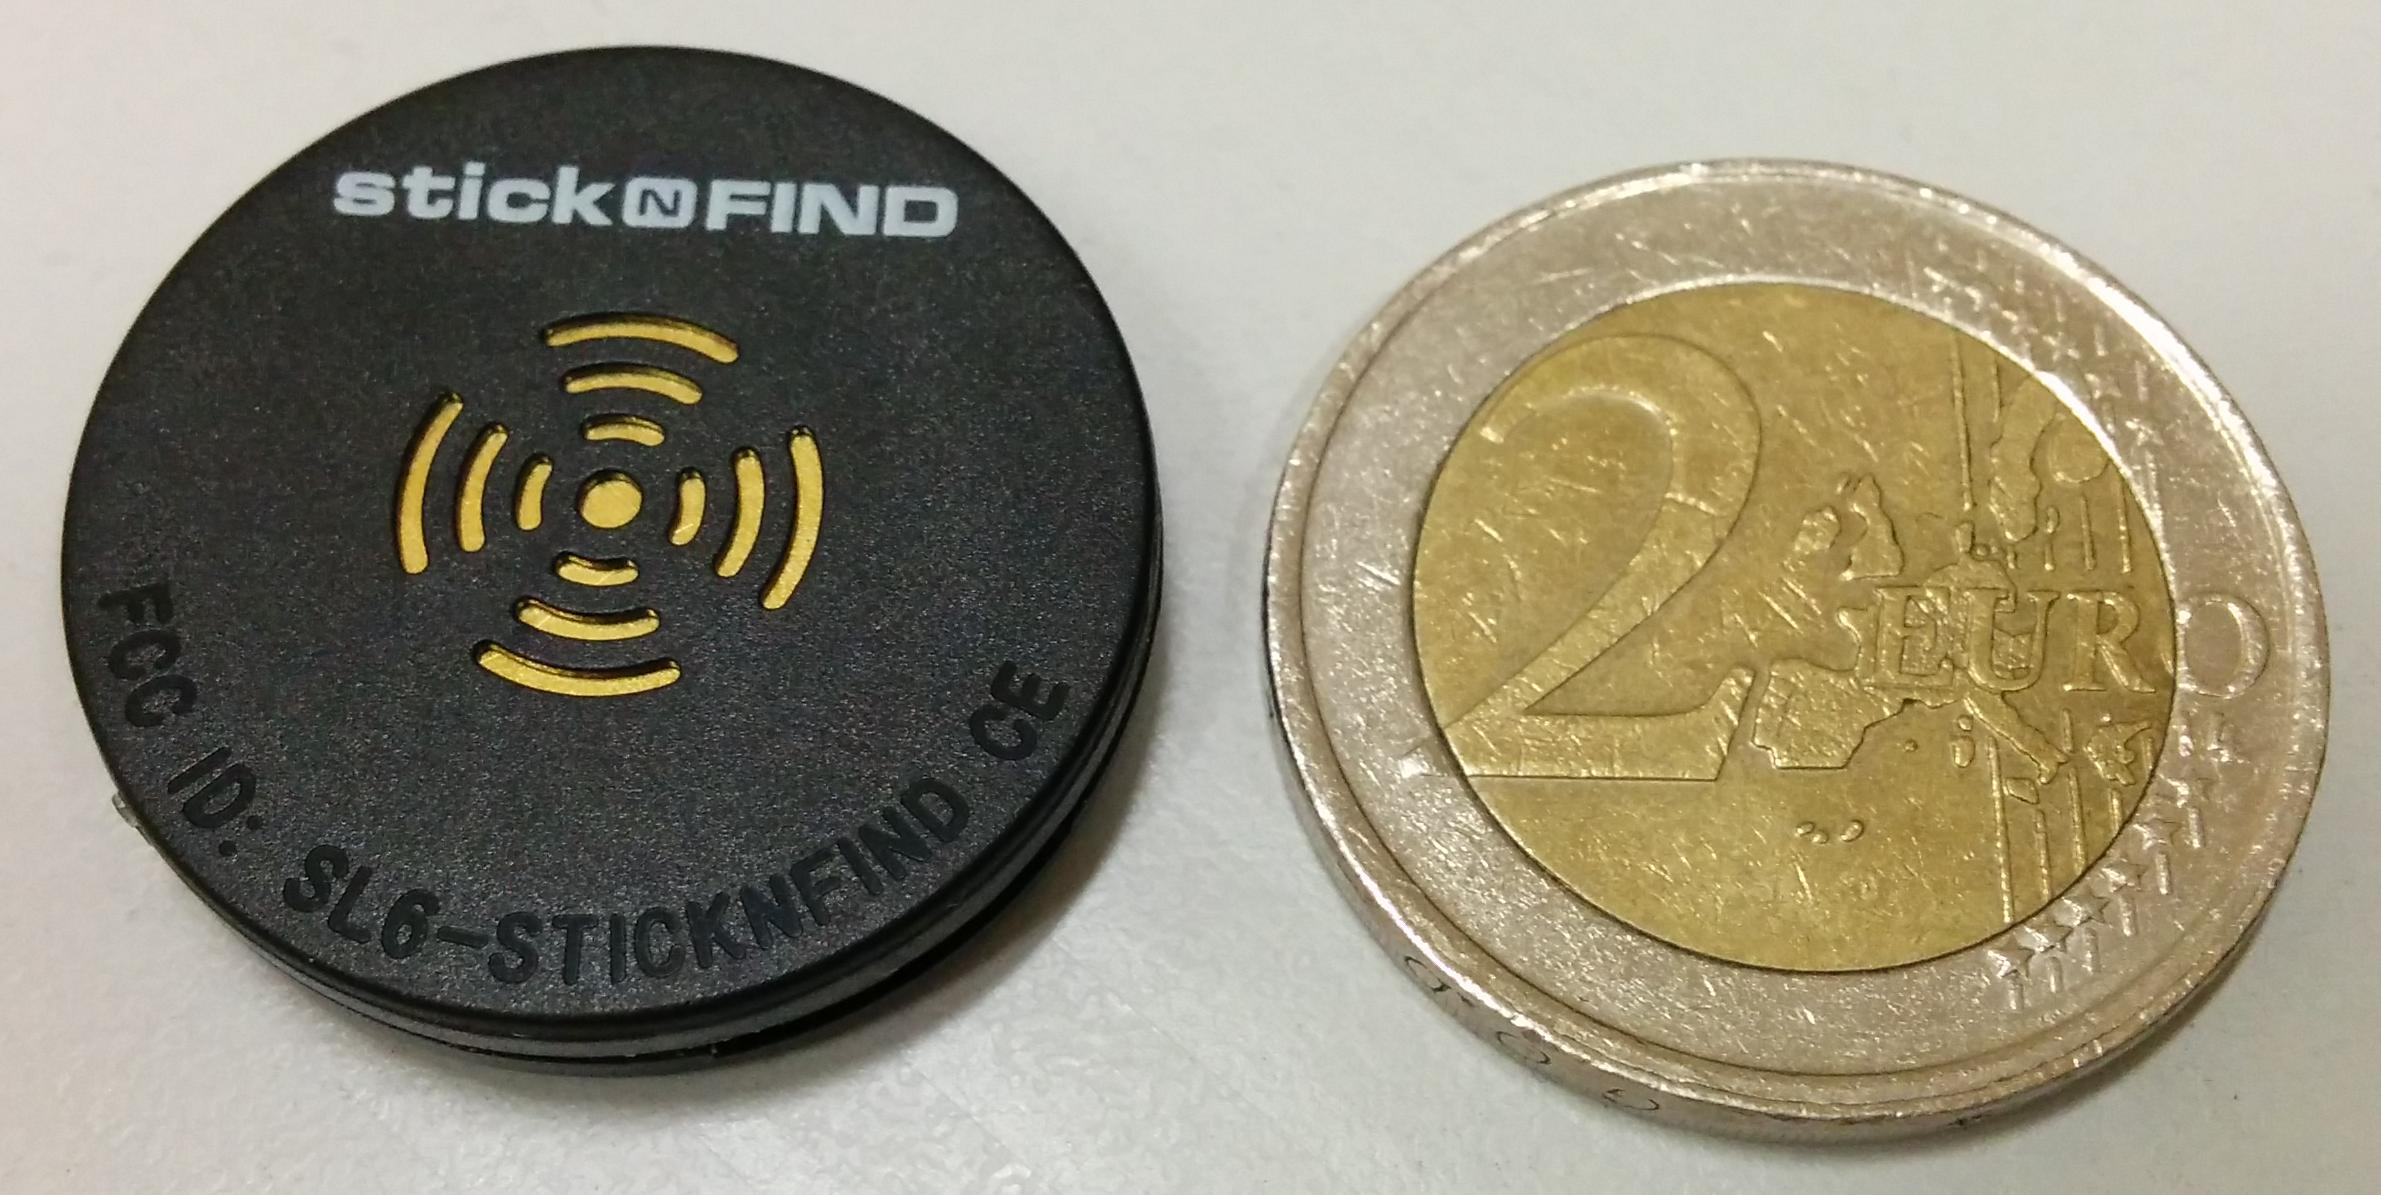
\includegraphics[width=0.99\textwidth]{img/ibeacon}
	\caption{
		A iBeacon, compared to a \EUR{2} coin.
	}
	\label{img:ibeacon}
\end{figure}

A technology which is often associated with Bluetooth but that is actually a separated and not compatible protocol is Bluetooth LE.
%
The reason why such technologies get associated is that, since the radio frequency used is the same (2.4GHz), dual mode devices can share a single radio antenna.
%
LE stands for Low Energy, and it is the main difference between the two protocols: at the expense of some bandwidth, Bluetooth LE consistently reduce the amount of energy required.
%
Bluetooth LE applications are particularly interesting, and range from health care to fitness to alerts to proximity sensing.

Proximity can be estimated using the received signal strength indicator (RSSI), and the very low power consumption of Bluetooth LE allowed for the realisation of electronic leashing systems, namely systems where an electronic device is paired to an object and can be used in order to compute the relative position.
%
The applications are, for instance, finding of misplaced, out-of-sight devices (when the electronic device is paired with a movable object) and indoor localisation (if the electronic device is located on a still standing object).
%
Relying on this technology, Apple created iBeacon, namely very small (coin sized, see \Cref{img:ibeacon}) electronic devices consisting basically of a battery and a Bluetooth LE device.
%
iBeacons can be attached to objects, and they send a universally unique identifier (UUID) to enabled smartphones in range.
%
If the smartphone can associate the UUID with a position, it can deduce its location relative to the iBeacon.
%
The low energy feature plays a fundamental role in this kind of applications: beacons whose battery would last few hours would be of little practical use.
%
With current technologies, a beacon device can be powered by a standard, rather cheap battery for several months, up to a couple of years.
%
This technology is probably the prelude to precise indoor localisation. 

\subsection{NFC}

\begin{figure}
	\centering
	
\includegraphics[width=0.99\textwidth]{img/nfc-tag}
	\caption{
		Two NFC tags, mounted on stickers.
		%
		In order to understand the size, they are placed above a Samsung Galaxy S3, a 4-inches smartphone.
		%
		Moreover, smaller versions of such tags exists, the models pictured here are very common-sized.
	}
	\label{img:nfc-tag}
\end{figure}

Near Field Communication, or NFC, is a technology designed for low energy communication between two devices in proximity (typically few centimetres).
%
It is designed for low energy consumption rather than high bandwidth: its speed (depending on the specification) ranges from 126kb/s to 242kb/s.

One of the most interesting features of NFC is that one of the two devices (the so-called ``tag'') can be completely passive, and still carry a small amount of information within (currently between 96 and 4096 bytes).
%
No battery or energy source is required, the information included can be read by active NFC devices in proximity.
%
Having no need of battery at all, NFC tags can really be tiny, even smaller than iBeacons.
%
\Cref{img:nfc-tag} shows two NFC tags: compared with iBeacons, they can be much lighter and thinner.
%
Brought to the world of humans, it is something like creating a sticker with very small sized text: those who have a powerful enough magnifying glass and are close enough to use it properly can read what it says.

The range of applications of such technology is rather broad.
%
The one which was probably most sponsored is contact-less payment, namely the ability to pay just tapping the phone close to the check-out counter.
%
This is a very interesting possibility, and indeed in 2007 there were enthusiastic forecasts \cite{nfc2007} about its quick diffusion, that did not happen as quick as expected.
%
A number of studies tried to understand the reasons behind this slow adoption, and it appears that reasons are more correlated to marketing and management rather than technological maturity \cite{nfc-diffusion-reasons, nfc-diffusion-europe, nfc-diffusion-asia}.
%
Similarly, if the phone stores identity or access tokens, NFC is a very suitable technology for effectively using such tokens: in this case, its very low range is a nice feature.
%
NFC can also be used as a technology enabler, namely as a mean to securely bootstrap another connection, or join a local network of devices.
%
An example of such use is the Android Beam technology, that relies on NFC in order to establish a Bluetooth connection between two Android devices, transfer a file, then close the Bluetooth connection.
%
Technically, NFC could be used to directly transfer files, but both WiFi and Bluetooth offer much wider bandwidths and range, and as a consequence are preferred for such task.
%
Another interesting application field is mobile device automation: it is achieved by attaching
%
Generally speaking, NFC comes in handy when there is need of a communication mean whose range should be very limited.


\section{Towards a P2P pervasive continuum?}

We are living exciting times.
%
In about five years from the introduction of the technology on the market, almost everybody got a personal smart device always with her.
%
Miniaturisation and power efficiency is constantly growing at a stunning rate, allowing data, communication systems and computation to be spread around in our physical world.

In few decades, we will probably witness the diffusion on computation on everyday object.
%
In such a scenario, the device density will be much higher if compared to the current, up to the point that the aggregation of devices participating the system could be seen as a ``pervasive continuum'' \cite{sapere-procedia7}.
%
This continuum is studied under a number of names, including pervasive computing, smart cities, and the Internet of Things, in order to provide a wealth of services in an un-intrusive manner \cite{ker2014,Conti12,zam12,Harnie12}.

One of the possible strategies is to connect every single device to the Internet, aggregate its information in a remote server, do the necessary computation, then send back eventual results where they are needed.
%
This is the strategy behind cloud computing, which is achieving great success.
%
In particular, we argue, this strategy is interesting when the information could or should be aggregated with information from other, distant sources, or conserved for historical purposes.
%
This path, however, gets harder and harder to follow with device density: besides the obvious increasing on the total information produced, and consequently of the information to transmit and process, there are two other problems: the saturation of the wireless medium, and the locality of information.

Who tried to use its own smartphone in a very crowded environment has probably experienced connection or network issues.
%
The problem, as discussed in \Cref{International Mobile Telecommunications}, is that current technology must share a common medium among all the devices in the same area.
%
Increasing the maximum number of devices per area is one of the goals of the next generation of international mobile telecommunication technologies.
%
One of the proposed approaches is to switch to a very dense array of very small cells by deploying multiple antennas at a very short distance one another, e.g. inside the public illumination poles.
%
Devices nearby the local antenna would connect to it, and the antenna would then connect them to the rest of the network transparently, in a way somehow similar to the current WiFi ``infrastructure mode''.
%
Clearly, diffusing such antennas can possibly represent a major infrastructural upgrade, and, potentially, cost.

Another observation is that not every device needs direct access to the Internet to be able to accomplish its task, and this is increasingly true with increased density.
%
Thinking about today's devices, let's consider the current smartwatches and fitbands: the former relies on a smartphone or tablet in order to provide Internet-based services, and the latter uses no Internet connection at all, but just sends data to the smartphone to be processed.
%
Along the line of favouring locality, there is a second advantage which relates to privacy issues: there is no reason to send personal information away, if the system does not need data from distant points nor requires more computational power of the amount available locally.
%
Privacy issues gain great attention recently, especially after the leaks of classified information started in 2010 on Wikileaks and continued with the more recent leaks by Edward Snowden.
%
The content of such documents raised greater attention to privacy issues from general public.

A possible path which would help in both those directions (reduce wireless medium usage and keep data as local as possible) is the usage of local, possibly peer-to-peer interactions.
%
This way of organising communication is already exploited by existing applications.

One notable example is Firechat \footnote{\url{https://opengarden.com/firechat}}, which got particularly spotlighted during the ``Umbrella revolution'', namely the sequence of protests that took place in Hong Kong in 2014.
%
Similarly to what was done during Arab springs in 2011 \cite{arab-spring}, protesters relied on Internet services to organise and coordinate themselves.
%
The Chinese government policy on internet is not exactly a bright example of openness and neutrality \cite{china-censorship}, and services such as Facebook adn Twitter, widely exploited during Arab springs, were already effectively blocked in the land.
%
In short time, other social network were closed (such as Instagram), in order to cut protesters' communication means.
%
At that point, protesters had to find a communication system free of centralisation in order to prevent targeted Internet filters, and Firechat was the answer.
%
Firechat is a messaging application for mobile phones that, when the smartphone has access to the remote Firechat cloud, works as other more famous alternatives, such as WhatsApp\footnote{\url{http://www.whatsapp.com/}} and Telegram\footnote{\url{https://telegram.org/}} do.
%
When no access to Firechat servers is available, then the software tries to reach the destination by spreading the message hop-by-hop, building a de-facto mesh network.

Another interesting experiment is Serval Mesh \cite{serval-mesh}.
%
Serval Mesh accomplishes similar tasks, but it also supports calls and file transfers besides messaging.
%
Its main goal is to provide a networking among users who are in an area where there is no Internet access at all, for instance because of a disaster event.
%
It relies on WiFi to create a ad-hoc peer-to-peer network among devices.
%
Due to this lower level aspect, Serval Mesh requires privileged access to the hardware and some higher skill than Firechat, which is easier to setup but requires the availability of a Internet connection.
%
In \cite{mesh-network-telephony}, Serval Mesh is used to build an alternative, purely peer-to-peer telephony network.

Despite the existence of such mesh-oriented applications, however, a general and widespread approach for easily design and program the devices that compose our pervasive continuum is still under investigation \cite{Ray13}.
%
The most consistent contribution of this thesis is devoted to the research of general, well engineered approaches to build such systems.

\chapter{Self-organisation}
\label{coordination-infrastructures}

In \Cref{pervasive-devices} we took a look to the world of pervasive devices, also describing their communication means and hypothesising the near future development.
%
In this chapter, we focus on the software, and in particular on the challenges of engineering the development of software that will run on an ensemble of pervasive devices.
%
We first discuss the issue of coordination and self-organisation: how do we make all those possibly devices collaborate together in order to achieve a global goal, without a centralised decision-maker?
%
Which software platform may we devise to ease this operation?
%
We will see that similar problems have already been successfully solved in nature: the mechanisms underlying such natural behaviours, can, if properly mimicked, help to realise solutions in software systems.
%
We will then run through the existing literature on the issue, analysing the existing platforms supporting pervasive computing, and the tools that can be used to test and debug applications prior to deployment.
%
Finally, we will discuss the shortcomings of the existing technology, and pave the way for the contribution of this PhD thesis.

\section{Software ecosystems}

Regardless the name that we want to use, being it ``Internet of Things'' rather than ``Smart cities'' or ``Pervasive computing'', in all cases we are talking about a system that is expected to host many computations that feature, according to \cite{ker2014}:
\begin{description}
\item[Situatedness] | Pervasive services are typically time- and space-dependent, and feature physically- or socially-situated activities. Components of pervasive systems should be able to interact with the surrounding physical and social world by adapting their behaviour accordingly.
%
\item[Autonomy and self-adaptivity] | While individual components should be autonomous in the face of the inherent dynamics of their operational environment~\cite{agents-ieeecn6}, pervasive systems should also feature \emph{system-level autonomy} to deal globally with the unpredictability of the environment, providing properties such as self-adaptation, self-management, and self-organization~\cite{Mam06}.
%
\item[Prosumption and diversity] | Infrastructures for pervasive systems must promote open models of component integration, to be able to take advantage of the injection of new services and components~\cite{ZamO04}. This is particularly true in the context of \emph{socio-technical systems}~\cite{interactioncomplexity-iccci2013}, where human users and software agents act as \emph{prosumers} -- both consumers and producers -- of devices, data, and services.
%
\item[Eternity] | As well as short-term adaptation, a pervasive systems infrastructure should allow for the long-term evolution of organizations, components, and patterns of usage, in order to accommodate technological advances as well as the mutable needs of users without requiring extensive re-engineering effort~\cite{softwareevolution-iwpse2005}. In fact, pervasive systems are better conceived as \emph{eternal} systems, engineered for continuous, unlimited service, upgrading, and maintenance over time.
\end{description}

At the same time, ``traditional'' networks are also increasing in scale and importance for enterprises both large and small.
%
In an increasingly information-dependent and interconnected world, the rising cost of managing and maintaining such systems is driving a search for solutions that can increase the autonomy of computing systems, enabling them to act more as collective services than individual machines~\cite{eze2012autonomic, hu2011cloudreview}, and continuing working over time.
%
In both of these cases, and a number of other areas facing similar challenges (e.g., large-scale sensor networks, multi-UAV control), there is a growing recognition that new paradigms are needed to face the challenge of coordination, namely, engineering the space of interactions \cite{Wegner}.
%
The goal of such engineering paradigms is to find reliable processes that lead to self-organising aggregates that act more as a collective service than as individual machines \cite{Cabri03,Bis11,Social12,PSC13}.

\section{Nature inspiration}

Natural systems are good in dealing with the \emph{complexity} of coordinating large-scale software ecosystems \cite{nic-ieeeis19,facets,nic-cacm49}, since they natively feature key properties such as autonomy, openness, fault tolerance, situated behaviour, self-adaptation and robustness.
%
Many specific models have been proposed in literature, taking inspiration from natural ecosystems, social insects, biochemistry, chemistry and also physics \cite{ecosystems-jpcc7}.

\subsection{Physical-inspiration}

To the category of physical inspired systems belong all those works that take inspiration on the way physical particles move and self-organise according to gravitational and electromagnetic forces.
%
For instance, in \cite{fieldbasedcoordination-mamei06}, computational ``force fields'' -- generated either by coordinated components or by the coordination middleware -- propagate across a spatial environment, leading to distributed data structures that affect the actions and motions of the agents in that environment.
%
A similar approach is proposed in Co-fields \cite{cofields--esawIII}, exploiting composite computational fields to coordinate the motion of users and robots in an environment.
%
Physical inspiration also has influenced self-assembly, for instance in \cite{guo2012} the adoption of virtual force fields is suggested in order to control the material's shape.

\subsection{(Bio)chemical-inspiration}

Chemical reactions can be seen as an ensemble of myriads of simple laws that generate and regulate the evolution of extraordinarily complex molecular structures.
%
Those rules coordinate in some way the behaviours of a huge number of components, up to the point where they reductionistically drive the evolution of complex assemblies such as biological organisms and meteorological systems.

Gamma \cite{gamma-scico15} was the first and the most prominent example of a chemically-inspired model.
%
In Gamma, coordination is conceived as the evolution of a space governed by chemical-like rules, globally working as a rewriting system \cite{gamma-lncs2235}.
%
In the CHAM (chemical abstract machine) model \cite{cham-tcs96}, states are interpreted as chemical solutions, where floating molecules (representing coordinated entities) interact according to some reaction rules, and where \emph{membranes} constrain the execution of reactions.

In chemical tuple spaces \cite{chemcoord-soarbook} data, devices, and software agents are uniformly represented in the form of chemical reactants, and system behaviour is expressed by means of full-fledged chemical-like laws that are both time-dependent and stochastic rather than in form of rewriting rules.
%
\emph{Biochemical tuple spaces}~\cite{VCMZ-TAAS2011} enhance chemical tuple spaces by shaping coordination through distribution and topology.
%
Biochemical coordination models appear very flexible in enabling the spatial formation of both localised and distributed activity patterns, and have been exploited in many special-purpose pervasive frameworks, including crowd mobility management~\cite{werfel} and participatory sensing~\cite{lee}. The amorphous computing model can be considered an example of biochemical coordination model~\cite{amorphous}.

Beside having been conceived as general computational model, (bio)chemically-inspired computing can be an effective starting point to realize schemes of dynamic service composition~\cite{frei} or knowledge aggregation~\cite{mariani2013molecules}.
%
Network protocols for data distribution and aggregation according to chemical models have also been explored, as in the Fraglets approach~\cite{Meyer07,Monti13}.
%
Several proposals exist to support service composition based on chemical models~\cite{BanP09}, including proposals specifically conceived for adaptive pervasive services~\cite{cpe}, or to support the adaptive organization of knowledge~\cite{mariani2013molecules}.

\subsection{Stigmergy}

In the computer science literature, the term ``stigmergy'' refers to a set of nature-inspired coordination mechanisms mediated by the environment~\cite{stigmergyhistory-artificiallife5,stigmergy-artificiallife5}.
%
Agents deposit data into a distributed, shared, environment so as to collectively (yet implicitly) build distributed data structures that can help them navigate in such environments.
%
The notion of \emph{stigmergy} was introduced in \cite{stigmergy-grasse59} as the fundamental coordination mechanism in termite societies.

Nowadays, the most widely-studied example of stigmergic coordination in insect societies is probably that of ant colonies~\cite{dorigo-aco2004}.
%
The basic mechanism is based on \emph{pheromones} that are released in the environment by the ants that find food on their way back to the nest, thus building pheromone trails towards food that other ants are then stimulated to follow.
%
The pheromones act as environment markers for specific social activities, driving both the individual and the social behaviour of ants.
%
For instance, digital pheromones \cite{pheromoncoord-aamas2002,stigmergy-e4masII} have been fruitfully exploited as the basic mechanism for coordinating the movements of robot swarms and modular robots~\cite{tota-aamas2005}, for helping people find directions in an unknown environment~\cite{MameiZ07}, and for efficiently cluster information in networks \cite{collectivesort-scico74,wordNet}.
%
In the area of networking, stigmergy has been exploited to realize effective routing mechanisms in dynamic networks~\cite{swarmintelligence-book1999,AC-Survey}.





\section{Spatial patterns}

%TODO: what is a pattern
Vedere se c'è qualcosa di utile in NACO \cite{FDMVA-NACO2012} o in \cite{GVO-CEEMAS2007}, o in \cite{ecosystems-jpcc7} o in \cite{BabaogluPatterns}

\subsection{Gossip}

%TODO% what is gossip

\subsection{Gradient}
\label{gradient}
A simple though paramount data structure that can be built upon this paradigm and that is a building block of many of the more advanced patterns is the spatial gradient, which assigns to each node a value $\varGamma$ depending on its position in time and space and on its context \cite{mamei2009acm,crf,VCMZ-TAAS2011}.
%
This structure originates in one or more devices called sources.
%
In every source device, $\varGamma=0$.
%
In every other device, let $N$ be the set of devices connected with it, and let $n$ be the n-th neighbouring device.
%
For this device, $\varGamma=[\min(f(n)) | n \in N]$: namely, the value of the device is the minimum of a function which operates on the neighbours.
%
For instance, if $ \forall n \colon f(n)=\varGamma_{n}+1$, where $\varGamma_{n}$ is the value of the gradient in $n$, then the local value will reflect the minimum hop count towards the nearest source.
%
If $f(n) = \varGamma_{n} +d(n)$ where $d(n)$ measures the actual distance from the device towards $n$, then the value of the gradient will approximate the distance from the nearest source.
%
Finally, along with the local value, a gradient can carry more information, e.g. some strings, the position of $n$, or numeric values.

% TODO problems with gradient
\cite{crf}

\subsection{Gradcast}

\subsection{Voronoi partition}

\section{Tuple-based coordination}

In a tuple-based coordination model \cite{coordbook2001--ch04}, software agents synchronize, co-operate, and compete based on \emph{tuples}, which are simple data structures representing information chunks.
%
Tuples are made available in \emph{tuple spaces}, which are shared information spaces working as the \emph{coordination medium}.
%
Coordination occurs by accessing, consuming, and producing tuples in an \emph{associative} way, relying on the actual content of tuples and not on any form of naming, addressing, or indexing.
%
An interesting survey of the technologies and platforms \cite{adaptivenesslinda-esoaI} analyses the suitability of tuple-based coordination systems in supporting openness, unpredictable changes in distributed environments, and several aspects related to adaptiveness: requirements that are of primary importance in pervasive systems.

Several implementations from both academia and industry exist.

\begin{description}
 \item[Anthill] \cite{anthill} is a framework meant to support design and development of adaptive peer-to-peer applications, in which each node is provided with a local tuple space, agents can travel the network and interact indirectly reading, writing and retrieving tuples.

 \item[Biochemical tuple spaces] \cite{biochemicalTupleSpaces}

 \item[GigaSpaces]\footnote{\url{http://www.gigaspaces.com}}

 \item[JavaSpaces] \cite{javaspaces1999,javaspaces}

 \item[Lime] \cite{murphy2006lime}

 \item[Linda] \cite{linda-toplas7} is the common ancestor of every tuple based coordination framework.

 \item[Molecules of knowledge] \cite{mariani2013molecules}

 \item[SwarmLinda] \cite{swarmlinda}

 \item[T Spaces] \cite{tspaces-ibmsj37}

 \item[TOTA] \cite{mamei2009acm, tota2} is a tuple-based middleware explicitly conceived to support field-based coordination for adaptive context-aware and spatially-aware activities in pervasive computing scenarios.
 %
 In TOTA, each tuple also carries with it a diffusion rule and a maintenance rule in addition to a content. Tota inspired other works, such as the evolving tuples model \cite{evolvingtuples}, which adds to the tuples a form of context awareness, in form of possible evolution and adaptation to environmental changes.

 \item[TuCSoN] \cite{tucson-aamas99}

%  \item[] \cite{}
%  \item[] \cite{}
%  \item[] \cite{}
%  \item[] \cite{}
%  \item[] \cite{}
%  \item[] \cite{}
%  \item[] \cite{}
%  \item[] \cite{}
\end{description}

SELFMAN? \cite{selfman}

MARS?

Plastic? \cite{plastic}

\cartago{}? \cite{RPV-JAAMAS2011}

\subsection{SAPERE}
\begin{figure}
\centering
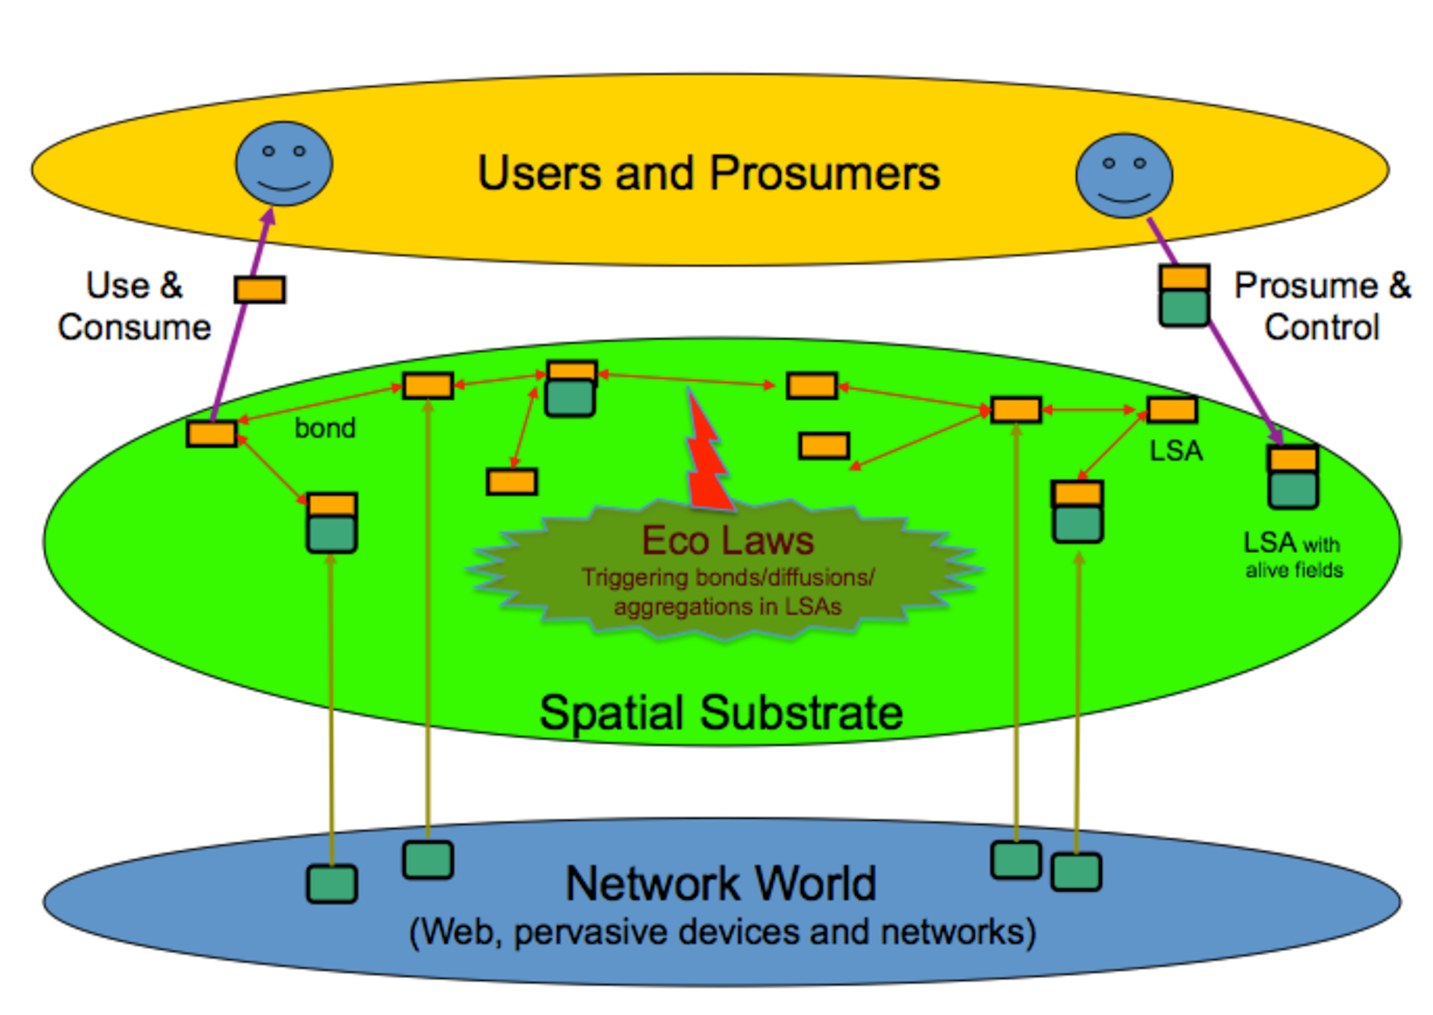
\includegraphics[width=0.99\textwidth]{img/architecture_2.pdf}
\caption{The SAPERE Reference Architecture.}
\label{img:sapere-architecture}
\end{figure}

SAPERE\footnote{The model was developed as part of an EU-funded research project. See \url{http://www.sapere-project.eu/}.} \cite{sapere-procedia7} is a nature-inspired coordination model and framework to support the design and development of composite pervasive service systems.
%
Its reference architecture and coordination model synthesize from existing nature-inspired approaches, such as \cite{biochemicalTupleSpaces, frameworkSelfOrg, VCMZ-TAAS2011, wordNet}, and is based on an assumption of spatial, local interactions (to be realized via a network of distributed tuple spaces), which is in line with all nature-inspired approaches.
%
Its coordination laws make it possible to express and deploy general nature-inspired distributed algorithms and coordination patterns.
%
SAPERE abstracts a pervasive environment as a non-layered \emph{spatial substrate} deployed upon a dense network of connected heterogeneous ICT devices (\Cref{img:sapere-architecture}).
%
SAPERE acts as a shared coordination medium embodying the basic laws of coordination.
%
Its core components are \cite{sapereecolaws-sac2012}:
\begin{description}
 \item[LSA] Because of the need to tolerate diversity, a cornerstone of pervasive ecosystems is that a uniform representation is required for the various software agents living within them (whether they run on smartphones, sensors, actuators, displays, or any other computational device).
 %
 Such a representation needs to expose any information about the agent (state, interface, goal, knowledge) that is pertinent for the ecosystem as a whole or for any subpart of it.
 %
 In SAPERE this description is called ``Live Semantic Annotation'' for it should continuously represent the state of its associated component (live), and it should be implicitly or explicitly connected to the context in which such information is produced, interpreted and manipulated (semantic)—possibly relying on standard technologies and techniques of the Semantic Web, like RDF \cite{manola2004primer}.
 %
 \item[LSA-space] To handle situatedness, the behaviour of each agent strictly depends on the local context in which it runs, that is, on the state of other agents living in the same locality (intended as network neighbourhood).
 %
 As such, the LSAs of each agent are reified in a distributed space (called an “LSA-space”) acting as the fabric of the ecosystem, where “context” is simply defined and represented as the set of LSAs stored in a given locality.
 %
 \item[LSA bonding] Additionally, and in order to make any agent act in a meaningful way with respect to the context in which it is situated, special mechanisms are needed to provide a fine-tuned control of what to each agent is visible/modifiable and what is not.
 %
 SAPERE tackles this issue by allowing an LSA to include bonds (i.e., references) to other LSAs in the same context.
 %
 It is only via a bond that an agent can inspect the state/interface of another agent and act accordingly, while modifications are allowed only to the LSAs an agent injected itself.
 %
 \item[Eco-laws] Because of adaptivity, while agents enact their individual behaviour by observing their context and updating their LSAs, global behaviour (i.e., global system coordination) is enacted by self-organising manipulation rules of the LSA-space, called eco-laws.
 %
 They can execute deletion/update/movement/re-bonding actions applied to a small set of LSAs in the same locality.
 %
 SAPERE structures such eco-laws as chemical-resembling reactions over LSAs—similarly to other approaches like \cite{BanP09,biochemicalTupleSpaces,VCMZ-TAAS2011}.
\end{description}

\section{Aggregate programming}

\begin{figure}
\centering
\subfigure[Continuous Space]{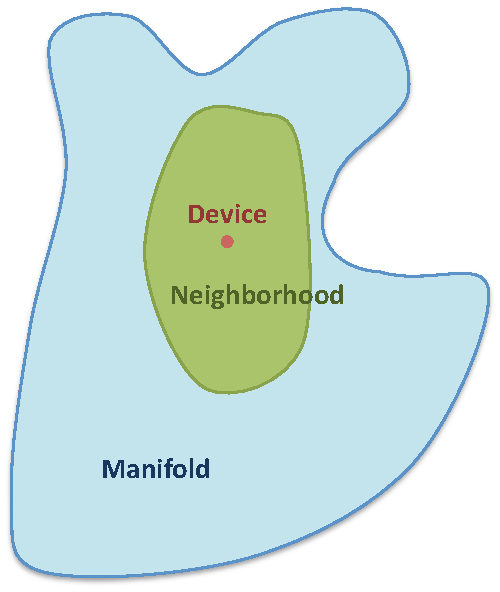
\includegraphics[width=0.45\columnwidth]{img/space-continuous}\label{img:medium}}
\hspace{0.01\columnwidth}
\subfigure[Discrete Network]{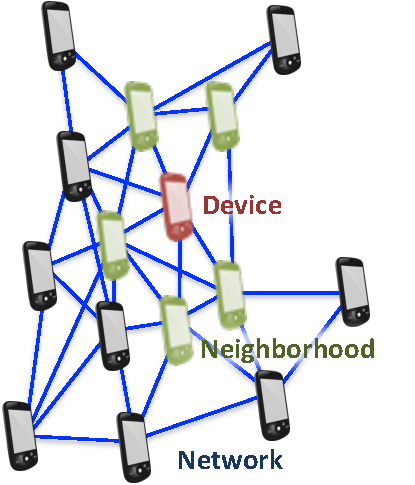
\includegraphics[width=0.45\columnwidth]{img/space-discrete}\label{img:mediumnet}}
\caption{Computational field models originate from approximation of continuous
space (a) with discrete networks of devices (b).}
\label{img:space}
\end{figure}

Aggregate programming is founded on the observation that in many cases the users of a system are much less concerned with individual devices than with the services provided by the collection of devices as a whole.
%
Typical device-centric programming languages, however, force a programmer to focus on individual devices and their interactions.
%
As a consequence, several different aspects of a distributed system typically end up entangled together: effectiveness and reliability of communications, coordination in face of changes and failures, and composition of behaviours across different devices and regions.
%
This makes it very difficult to effectively design, debug, maintain, and compose complex distributed applications.

Aggregate programming generally attempts to address this problem by providing composable abstractions separating these aspects:
\begin{enumerate}
 \item device-to-device communication is typically made entirely implicit, with higher-level abstractions for controlling efficiency/robustness trade-offs;
 \item distributed coordination methods are encapsulated as aggregate-level operations (e.g., measuring distance from a region, spreading a value by gossip, sampling a collection of sensors at a certain resolution in space and time); and
 \item the overall system is specified by composing aggregate-level operations, and this specification is then transformed into a complete distributed implementation by a suitable mapping.
\end{enumerate}

In short, the key idea behind aggregate programming is to provide languages and APIs that allow a distributed collection of devices to be programmed in terms of their collective behaviours, keeping outside the sight of the software designer details on how such coordination is actually implemented.

A large number of very diverse aggregate programming approaches have been proposed, including abstract graph processing (e.g.,~\cite{kairos}), declarative logic (e.g.,~\cite{Meld}), map-reduce (e.g.,~\cite{dean2008mapreduce}), streaming databases (e.g.,~\cite{tinydb}), and knowledge-based ensembles (e.g.,~\cite{SCEL})---for a detailed review, see~\cite{SpatialIGI2013}.

Despite the fact that all of them are based on viewing the collection of devices as an approximation of continuous space (as depicted in \Cref{img:space}), most aggregate programming approaches, however, have been too specialized for particular assumptions or applications to be able to address the complex challenges of these emerging environments.

\subsection{Proto}
\label{proto}

Proto language and middleware~\cite{proto} exploits field-based coordination to orchestrate the activities of sensor-actuator networks

Proto is based on the notion of a {\em computational field}---a map from devices comprising the system to (possibly structured) values, which is treated as unifying first-class abstraction to model system evolution and environment dynamics.

The programming constructs are combined together to form programs, whose semantics is defined in terms of a sequence of synchronous rounds of evaluation by a discrete network of devices called ``computational rounds''.
%
In practice, however, there is no requirement for synchrony, and each device can evaluate its own computational rounds independently.

Despite its qualities, Proto still lacks many features expected in a modern programming language and has an implementation encumbered by a number of obsolete considerations that make it difficult to maintain and extend.


\cite{proto}

\subsection{Field Calculus}
\label{field-calculus}

Field Calculus is an attempt to find a unifying model for programming \emph{computational fields} as a generalization of a wide range of existing approaches (Proto in particular, but also \cite{mamei2009acm,regiment,VCMZ-TAAS2011,tota2,nagpalphd,yamins,regiment}).
%
Formalized as the computational field calculus~\cite{VDB-FOCLASA-CIC2013}, this universal language appears to provide a theoretical foundation on which effective general aggregate programming platforms can be built.

Critically, although originally derived from continuous-space concepts, the calculus does not depend on them and is applicable to any network.
%
Field calculus is expressive enough to be a universal computing model~\cite{BVD-SCW14} but terse enough to enable a provable mapping from aggregate specifications to equivalent local implementations.

Field calculus~\cite{VDB-FOCLASA-CIC2013} hence provides a key theoretical and methodological foundation for aggregate programming.
%
Its aim is to provide a universal model that is suitable for mathematical proofs of general properties about aggregate programming and the aggregate/local relationship, just as $\lambda$-calculus~\cite{LambdaCalculus} provides for functional programming, $\pi$-calculus for parallel programming~\cite{PiCalculus}, or Featherweight Java~\cite{FJ} for Java-like object-oriented programming.

In the field calculus, everything is a field: computational fields are used to model every aspect of distributed computation, including input from sensors, network structure, environment interactions, distributed computations (e.g. progressive aggregation and spreading processes), and output for actuators.
%
In particular, field calculus is constructed using five basic constructs:
\begin{enumerate}
 \item function definition and evaluation;
 \item ``built-in'' operations for stateless local computation, e.g.,
addition, multiplication, reading a sensor;
 \item a time-evolution construct which allows for stateful computation;
 \item a neighbour-value construct that creates a field of values from a device's neighbours;
 \item a restriction operator to select which computations to perform in various regions of space and time.
\end{enumerate}

As well as in Proto, in Field Calculus the semantics of programs created by combining such constructs is defined in terms of a sequence of (possibly synchronous) ``computational rounds''.

The minimal syntax of field calculus has allowed its semantics, including proper coherence of device interactions, to be proven correct and consistent~\cite{VDB-FOCLASA-CIC2013}.
%
Additionally, despite its definition in terms of discrete semantics, field calculus is also space-time universal~\cite{BVD-SCW14}, meaning that it can approximate any field computation, either discrete or continuous, with arbitrary precision given a dense enough network of devices.

This, then, is the key contribution of field calculus: any coordination method with a coherent aggregate-level interpretation is guaranteed to be expressible in field calculus.
%
Such a method can then be abstracted into a new aggregate-level operation, which can be composed with any other aggregate operation using the rules of built-in functions over fields.
%
Moreover, it can have its space-time extent modulated and controlled by restriction, all while guaranteed that the relationship between global specification and local implementation will always be maintained.

\begin{figure}
\centering
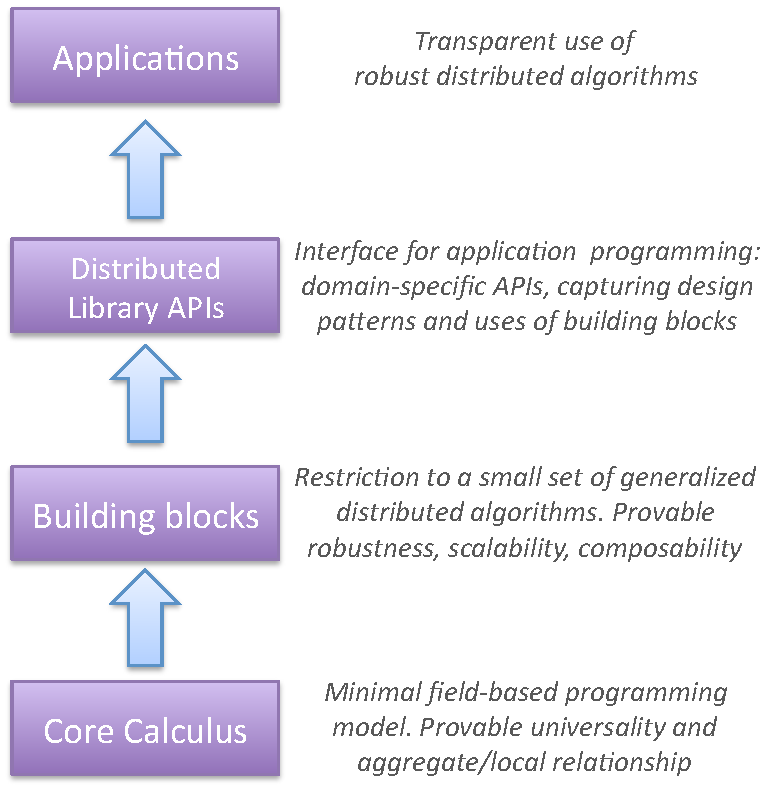
\includegraphics[width=0.99\textwidth]{img/aggregate-tower}
\caption{Layered approach for development of spatially-distributed systems via aggregate programming.}
\label{img:researchprogram}
\end{figure}

Such a core calculus, like any other, is more a theoretical framework than a practical programming language.
%
In practice, in fact, effective aggregate programming for real-world distributed applications is likely to require a layered approach such as the one depicted in \Cref{img:researchprogram}, of which field calculus represents the first block.
%
Some of the prior approaches on which field calculus is based provide very similar semantics (most notably Proto), but they all suffer from some combination of design and implementation problems that render them impractical for widespread adoption.
%
Besides Proto, which is probably the closest to a practical programming environment and whose problems have already been described in \Cref{proto}, others, such as \cite{VPB-COORD2012}, have only minimal implementation.

\subsubsection{Alignment}


\section{Engineering and tools}
\label{engineering-and-tools}

Despite the efforts of addressing specific aspects of self-adaptability and openness in pervasive contexts \cite{Mam06,BabaogluPatterns,facets}, yet a comprehensive engineering framework is missing.
%
The hardest challenge is due to the fact that most of the complexity of such systems does not come from the individual behaviours, but rather from interaction \cite{Wegner,interactionbook,interaction-interbook}.


Multiple methodologies have been proposed to tackle complex pervasive systems \cite{MCOV-SCP2011,BabulakIJOE2008,BandiniJASSS2009,josMacalN10,sapere-procedia7}, and they always include \emph{simulation} as a key step  to realise what-if analysis prior to actual development, to both assess the general validity of the designed mechanisms and to fine tune system parameters.
% TODO: need of simulation %
There are many kinds of simulation tools available: they either provide programming/specification languages devoted to ease construction of the simulation process, especially targeting computing and social simulation (e.g. as in the case of multi-agent based simulation \cite{BandiniJASSS2009,SchumacherCEEMAS2007,vizzari-massimulationbook09,repast,sklar2007al}), or they stick to quite foundational computing languages to better tackle performance, mostly used in biology-oriented applications \cite{Priami1995,murata1989,UhrmacherWSC2005,EwaldJOS2007}.
%
None of the existing tools, however, aims at bridging the gap between these approaches, trying to extend the basic computing model of chemical reactions -- still retaining its high performance -- toward ease applicability to complex situated computational systems.



\subsection{General purpose frameworks}
MASON \cite{luke2005simulation}, Repast \cite{repast}, NetLogo \cite{sklar2007al} and Swarm
\subsection{Specific simulators}
network simulators (the one, ns2)
biological simulators (ask Sara)

Specific per-use simulators, gener

\chapter{Shortcomings of coordination infrastructures}
\section{Engineering emergence}
\section{Local to global}
\chapter{Shortcomings of existing tools}
\section{Specific tools: expressiveness}
\section{General purpose tools: performance}

\part{Contribution}
\label{contribution}
\chapter{An integrated toolchain for pervasive ecosystems}

We discussed in \Cref{engineering-and-tools} the importance of simulation in the engineering process of designing pervasive ecosystems.
%
In this chapter, we will discuss one of my contribution to this research branch, namely the development of an integrated tool named \alchemist{}, which has been inspired by chemical oriented simulators.
%
We first talk about chemical inspiration, and how existing chemical-oriented stochastic simulation algorithms (SSAs) can be extended towards higher flexibility, up to the point that they become suitable to simulate potentially complex environments, still retaining their high performance.
%
To do so, our first effort will be to take an efficient SSA implementation and convert it to a general-purpose discrete event simulator (DES).
%
We then devise a meta-meta-model, complex and flexible enough to support the definition of middleware-specific meta-models.
%
Finally, some meta-models are presented.
%TODO: expand
%

\section{Chemical-inspired engine}
\label{chemical-engine}
In the following, we present a discrete event simulation engine derived from the popular and successful Gillespie's stochastic simulation algorithm \cite{gillespie1977}, and in particular from its notable and more efficient extensions developed by Gibson-Bruck \cite{gibson2000} and by Slepoy \cite{slepoy2008}.   
%
Gillespie's SSA is a discrete and stochastic method that intrinsically owns the event-driven properties \cite{spatialeventgillespie}: introduced to model chemical systems, nowadays it represents the basis of many simulation platforms, in particular those developed for the investigation of biochemical systems \cite{Priami:2001,Kierzek01032002,CiocchettaH09,versari08,montagna-cs2bio10,btssoc-jos7,Hoops15122006}. 
%
With significative extensions, it was recently used to model artificial systems grounding on computational models inspired to chemical natural systems and ecology \cite{Montagna-MONET2012}.
%
Moreover, its optimised extensions \cite{gibson2000,slepoy2008} are very efficient, thus allowing really fast simulation runs.

%-------------------------------------------------------------------------------
\subsection{Gillespie's SSA as an event-driven algorithm}
%-------------------------------------------------------------------------------
First of all, we summarise the idea that the Gillespie's SSA is grounded on:
%
a chemical system is modelled as a single space filled with molecules that may interact through a number of reactions describing how they combine. 
%
The instantaneous speed of a reaction is called propensity and depends on the kinetic  rate of the reaction and on the number of molecules of all the reagents involved. 
%
For a reaction $i$ of the form:
$$ R_0 + R_1 \xrightarrow{r} P_0 + P_1 + \ldots + P_n$$
the propensity $a_i$ is defined as:
$$ a_i = r\cdot [R_0] \cdot [R_1] $$
where $[M]$ is the number of molecules of species $M$.
%
Given that, the algorithm relies on the idea that the system can be simulated by effectively executing the reactions one by one and changing the system status accordingly. 
%
Every algorithm follows four main steps:
%
\begin{enumerate}
	\item select the next reaction $\mu$ to be executed;
	\item calculate the time of occurrence of $\mu$ according to an exponential time distribution and make it the current simulation time;
	\item change the environment status in order to reflect this execution;
	\item update the propensities of the reactions.
\end{enumerate}
%
Such algorithm is event-driven in that it executes only one reaction/event at a time: it changes the state of the system and consequently the event list \emph{i.e.}. which other reactions/events can be executed from there.

%-------------------------------------------------------------------------------
\subsection{Gillespie's optimised versions}
%-------------------------------------------------------------------------------
This algorithm has been improved in various works in literature, particularly notable is the work in \cite{gibson2000} and \cite{slepoy2008}.
%
Both works optimise the base algorithm in two phases: the selection of the next reaction to execute and the update of the reaction pool -- pending event list -- once an event has been executed.
%
For the latter, they both rely on the concept of ``dependency graph''.
%
A dependency graph (DG) is a statically created directed graph in which nodes are all the reactions in the simulated system, and arcs connect a reaction \texttt{r} to all those that depend on it, namely, those whose triggering time should be updated as $r$ is executed.
%
For instance, if \texttt{r} changes the concentration of some molecule \texttt{m}, all those reactions that use \texttt{m} are to be properly re-scheduled as soon as \texttt{r} is fired.
%
Even though this optimisation does not affect the execution time in the worst case, it offers great benefits in the average case, since most of the reactions are not interdependent.

The selection of the next reaction to execute is where those improved algorithms differ most.
%
In Slepoy's work, the author divides reactions in groups based on their propensity: if $p_{min}$ is the lowest propensity, the first group contains those reactions whose propensity ranges from $p_{min}$ and $2 p_{min}$, the second those between $2 p_{min}$ and $4 p_{min}$, and so on.
%
Give those groups, an algorithm called ``Composition-Rejection'' (CR) is applied.
%
In the composition phase, a group is randomly selected in logarithmic time; in the rejection phase a reaction is chosen within a group by throwing two random numbers: the first one, between $0$ and the number of reactions in the group, identifies a reaction; the second one, between $0$ and the maximum propensity allowed for the group, is used to decide whether or not to actually execute the selected reaction.
%
In case the reaction is rejected, the rejection procedure is re-applied.
%
Given the way groups are built, there is at least a 0.5 probability that the rejection procedure concludes at each attempt.
%
On average, the CR algorithm requires five random numbers to be thrown.
%
This algorithm requires logarithmic time to select the next reaction with respect to the total number of groups, but the author argues which, since in most biological scenarios this number is constant, then the algorithm runs effectively in constant time.
%
In Gibson-Bruck, the same selection operation is made by computing a putative execution time for each reaction, and then using a binary heap data structure to sort them.
%
This way, the next reaction to execute is always the root node of the tree, and the selection is performed in constant time.
%
However, once the reaction has been executed, all the dependent reactions must be updated and re-sorted in the tree. In the worst case, this takes logarithmic time with respect to the number of reactions.

%-------------------------------------------------------------------------------
\subsection{From SSA to full fledged DES}
%-------------------------------------------------------------------------------

Both the Gisbon-Bruck's and Slepoy's schedulers are granted to correctly simulate a Poisson process.
%
However, in order to build a full-fledged DES engine, we must offer the possibility to schedule also non-Markovian events.
%
Imagine, for instance, that we want to simulate an agent that does an action every fixed time interval (e.g. a man walking).
%
This, clearly, is not a memoryless process.
%
We argue that Gibson-Bruck offers a more suitable base for a general purpose DES: in fact, its next reaction choosing mechanism is orthogonal to the way the putative times are computed.
%
This intrinsic feature allows to neatly separate the generation of times (namely, the time distribution of each event) and the actual scheduling (choice of which event should run next).
%
We chose the Next Reaction Method for \alchemist{}, and, consequently, the main simulation algorithm follows the basic steps listed in \Cref{algo:engine}.

\begin{algorithm}
\begin{distribalgo}[1]
\vspace{5pt}
\STATE{\texttt{cur\_time} $=$ 0}
\STATE{\texttt{cur\_step} $=$ 0}
\FOR{each node \texttt{n} in environment}
  \FOR{each reaction \texttt{nr} in \texttt{n}}
    \STATE{generate a new putative time for \texttt{nr}}
    \STATE{insert \texttt{nr} in DIPQ}
    \STATE{generate dependencies for \texttt{nr}}
  \ENDFOR
\ENDFOR
\WHILE{\texttt{cur\_time} $<$ \texttt{max\_time} \AND \texttt{cur\_step} $<$ \texttt{max\_step}}
  \STATE{\texttt{r} $=$ the next reaction to execute}
    \IF{\texttt{r}'s conditions are verified}
      \STATE{execute all the actions of \texttt{r}}
      \FOR{each reaction \texttt{rd} which depends on \texttt{r}}
	\STATE{update the putative execution time}
      \ENDFOR
    \ENDIF
    \STATE{generate a new putative time for \texttt{r}}
\ENDWHILE
\caption{Simulation flow in \alchemist{}}
\label{algo:engine}
\end{distribalgo}
\end{algorithm}

A second feature that we need in order to shift the paradigm from pure chemistry towards higher expressiveness is the possibility to simulate multiple, separate, interacting and possible mobile entities.
%
This requirement can be partly addressed by the notion of intercommunicating compartments \cite{CiocchettaH09,versari08,montagna-cs2bio10,btssoc-jos7}, in a way that allows to also model systems characterised by a set of connected volumes and not only a unique chemical solution.
%
The hardest challenge in simulating multiple compartments with an efficient SSA is in improving the dependency graph: reactions that could be interdependent but happen on separated compartments should not be marked as interconnected within the dependency graph.
%
Mobility makes everything even harder, since it may lead to the creation and disruption of communication channels between compartments, and consequently to simulation-time changes in the structure of such dependency graph.
%
Summarising, supporting dynamic environments with multiple mobile compartments require the dependency graph to become a dynamic data structure, which cannot be pre-computed at the simulation initialisation and kept static.

\subsubsection{Dynamic Dependency Graph}

There are multiple ways to conceive such dynamic data structure.
%
Ideally, it would be possible to just drop the optimisation or reuse the classic definition, in which case the triggering of a reaction in whichever compartment would cause the recalculation of the status of each potentially dependent event in every compartment.
%
This approach would lead to a massive performance impact, since the dependency computation is the most expensive operation.
%
As evidence, in \cite{slepoy2008} some charts show the difference between Gibson-Bruck and Slepoy et al. algorithms with and without a dependency graph: the result is very strongly in favour of the former.

A possibility for efficiently adapting a dependency graph to a network of compartments could be to define the input and output contexts for each reaction, namely the places where reactions respectively ``read'' their reactants and ``write'' their products.
%
Multiple contexts could be defined, we propose to adopt three levels: \localc{}, \neighborhood{} and \globalc{}.
%
In a purely chemical simulation, all the reactions have a \localc{} input context and may have either \neighborhood{} or \localc{} output context, depending on whether or not they send molecules towards other compartments.

Let $dep: R^2 \longrightarrow boolean$ be the function that is used to build the static dependency graph in every SSA: given two reactions \texttt{r1} and \texttt{r2}, $dep(\texttt{r1}, \texttt{r2})$ returns \texttt{true} if the propensity of \texttt{r2} may be influenced by the execution of \texttt{r1}.
%
In a multi-compartment scenario, \texttt{r1} influences \texttt{r2} (there is an oriented edge in the dependency graph connecting \texttt{r1} to \texttt{r2}) iff $dep(\texttt{r1},\texttt{r2})$ is \texttt{true} and:
\begin{itemize}
 \item \texttt{r1} and \texttt{r2} are on the same node OR
 \item \texttt{r1}'s output context is \globalc{} OR
 \item \texttt{r2}'s input context is \globalc{} OR
 \item \texttt{r1}'s output context is \neighborhood{} and \texttt{r2}'s node is in \texttt{r1}'s node neighbourhood OR
 \item \texttt{r2}'s input context is \neighborhood{} and \texttt{r1}'s node is in \texttt{r2}'s node neighbourhood OR
 \item \texttt{r1}'s output context and \texttt{r2}'s input context are both \neighborhood\ and the neighbourhoods of their nodes have at least one common node. 
\end{itemize}
%
The filters listed above greatly compact the number of edges of a dependency graph in most scenarios, with great benefits on the engine performance.
%
On top of this finer-grain locality concept, if the model supports compartment mobility, the dependency graph must support the dynamic addition and removal of reactions.

Adding a new reaction implies to verify its dependencies against every reaction of the system. In case there is a dependency, it must be added to the dependency graph. 
Removing a reaction \texttt{r} requires to delete all dependencies in which \texttt{r} is involved both as influencing and influenced.
Moreover, in case of a change of system topology, a dependency check among reactions belonging to nodes with modified neighbourhood is needed. It can be performed by scanning them, calculating the dependencies with the reactions belonging to new neighbours and deleting those with nodes which are no longer in the neighbourhood.

\subsubsection{Dynamic Indexed Priority Queue}

An issue that arises with addition and removal of nodes from the simulation is the possible unbalancing of the scheduling queue, that in the original work is realised as a binary tree of reactions, whose main property is that each node stores a reaction whose putative time of occurrence is lower than each of its sons.

\begin{figure}%[H]
  \begin{center}
    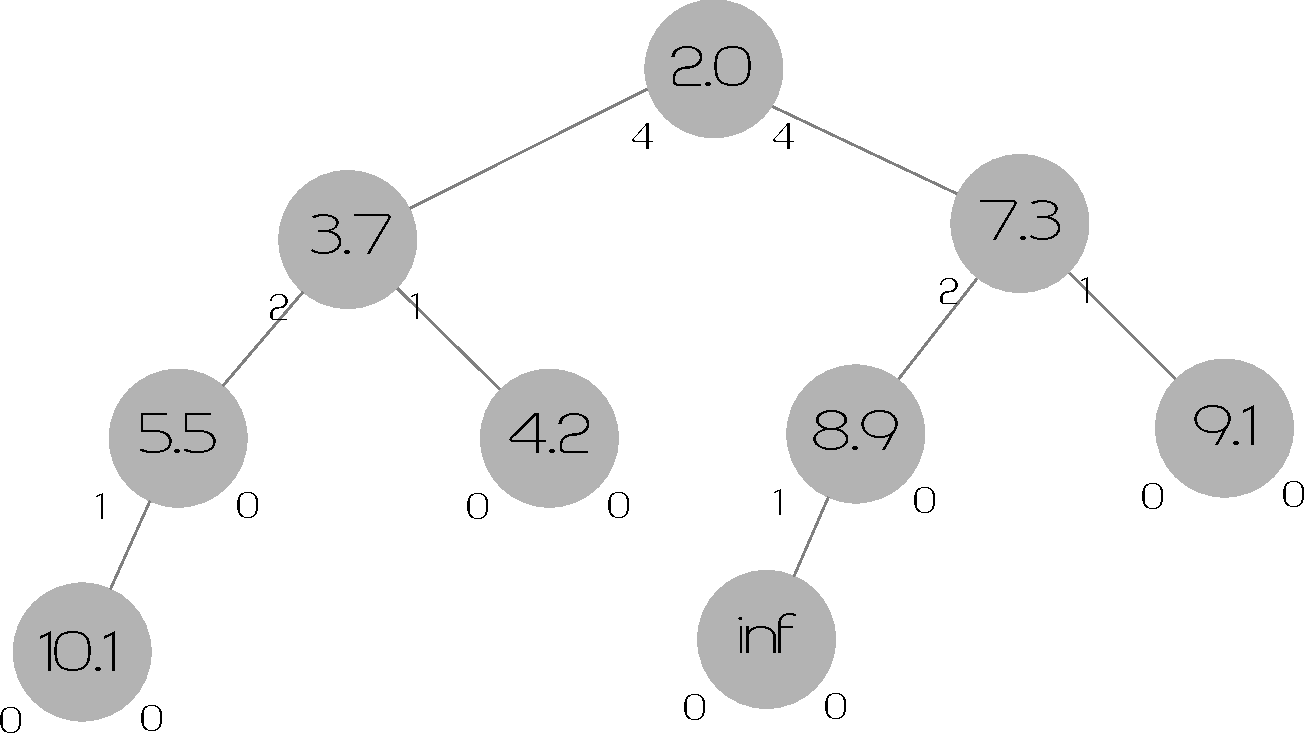
\includegraphics[width=0.99\textwidth]{img/extipq.pdf}
    \caption{Indexed Priority Queue extended with descendant count per branch}
    \label{img:ipq}
  \end{center}
\end{figure}

Our idea is, for each node, to keep track of the number of descendant per branch, having in such way the possibility to keep the tree balanced when adding nodes. In figure \ref{img:ipq} we show how the same IPQ drawn in \cite{gibson2000} would appear with our extension. Given this data structure, the procedures to add and remove a new node \texttt{n} are described respectively in \Cref{algo:newnode} and \Cref{algo:remnode}, in which the procedure \texttt{UPDATE\_AUX(n)} is the same described in \cite{gibson2000}.

\begin{algorithm}
\begin{distribalgo}[1]
\vspace{5pt}
\IF{root does not exist}
  \STATE{\texttt{n} is the new root}
\ELSE
  \STATE{\texttt{c} $\gets$ root}
  \WHILE{\texttt{c} has two descendants}
    \IF{\texttt{c.right} $<$ \texttt{c.left}}
      \STATE{\texttt{dir} $\gets$ right}
    \ELSE
      \STATE{\texttt{dir} $\gets$ left}
    \ENDIF
    \STATE{add $1$ to count of \texttt{dir} descendants}
    \STATE{\texttt{c} $\gets$ \texttt{c.dir}}
    \IF{\texttt{c} has not the left child}
      \STATE{\texttt{n} becomes left child of \texttt{c}}
      \STATE{set count of left nodes of \texttt{c} to $1$}
    \ELSE
      \STATE{\texttt{n} becomes right child of \texttt{c}}
      \STATE{set count of right nodes of \texttt{c} to $1$}
    \ENDIF
  \ENDWHILE
  \STATE{\texttt{UPDATE\_AUX(n)}}
\ENDIF
\caption{Procedure to add a new node \texttt{n}}
\label{algo:newnode}
\end{distribalgo}
\end{algorithm}

\begin{algorithm}
\begin{distribalgo}[1]
\vspace{5pt}
\STATE{\texttt{c} $\gets$ root}
\WHILE{\texttt{c} is not a leaf}
  \IF{\texttt{c.left} $>$ \texttt{c.right}}
    \STATE{\texttt{dir} $\gets$ left}
  \ELSE
    \STATE{\texttt{dir} $\gets$ right}
  \ENDIF
  \STATE{subtract $1$ to count of \texttt{dir} descendants}
  \STATE{\texttt{c} $\gets$ \texttt{c.dir}}
\ENDWHILE
\IF{\texttt{c} $\neq$ \texttt{n}}
  \STATE{swap \texttt{n} and \texttt{c}}
  \STATE{remove \texttt{n}}
  \STATE{\texttt{UPDATE\_AUX(c)}}
\ELSE
  \STATE{remove \texttt{n}}
\ENDIF
\caption{Procedure to remove a node \texttt{n}}
\label{algo:remnode}
\end{distribalgo}
\end{algorithm}

Using the two procedures described above, the topology of the whole tree is constrained to remain balanced despite the dynamic addition and removal of reactions.

\section{Meta-meta model}
\label{meta-meta-model}
The complexity of the systems we want to design is achieved by the following set of common key properties:
\begin{itemize}
 \item situatedness -- they deal with spatially- and possibly socially-situated activities of entities, and should therefore be able to interact with a limited portion of the surrounding world and contextualise their behaviour accordingly; 
 \item adaptivity -- they should inherently exhibit properties of autonomous adaptation and management to survive contingencies without external intervention, global supervision, or both; 
 \item self-organisation -- spatial and temporal patterns of behaviour should emerge out of local interactions and without a central authority that imposes pre-defined plans.
\end{itemize}

Among the many natural metaphors one can use as inspiration for modelling and developing artificial systems with the above properties \cite{ecosystems-jpcc7}, we consider chemistry following a series of work in the field of pervasive computing \cite{VCMZ-TAAS2011,VZ-INS2010,sapere-procedia7}. 
%
We argue that there are three main issues to be resolved in order to build a meta-model that can be sufficiently expressive for our purpose starting from a purely chemical model:
\begin{enumerate}
 \item the concept of environment where agents are situated and can move is missing in a model that considers only intercommunicating chemical compartments;
 \item the only available mean for changing the system status is the execution of a reaction;
 \item the only data item that chemical reactions can manipulate are molecules' concentrations, namely numbers connected to a particular token.
\end{enumerate}

In the following discussion, we will use interchangeably compartment/agent/node and reaction/events as synonyms.
%
As first step, we introduce the environment, absent in chemistry-derived SSAs, as first class abstraction.
%
The environment has responsibility to provide, for each compartment, a set of compartments that are its neighbours.
%
The rule which is applied to determine whether or not a node belongs to another node's neighbourhood  can be arbitrarily complicated.
%
Also, it is responsible of exposing possible physical boundaries, namely, to limit the possible movements of compartments situated within the environment.

The fact that reactions are the only abstraction the modeller can rely upon in order to let the simulated system progress is not a difficult problem by itself.
%
In fact, nothing prevents to widen the generality of a reaction by defining it as: ``a set of conditions that, when matched, trigger a set of actions on the environment''.

With this definition in mind, a condition is a function that associates to each possible state of the environment a numeric value ranging from zero to positive infinity.
%
If such value is zero, the event can not be scheduled; otherwise, it is up to the reaction to interpret the number: it can influence or not the time at which the reaction will be scheduled, depending on the specific reaction implementation.
%
In case we desire to re-build the original chemical model, we would define a condition for each of the molecules on the left-hand side of the chemical reaction that return the number of molecules currently available in the local compartment.
%
Also, we would define the reaction in such a way that it correctly interprets the number returned by the conditions as concentration of each reactant and correctly applies the rules for computing a propensity to be used to influence the reaction speed \cite{gillespie1977}.

In this framework, actions are arbitrary changes of the environment.
%
In case of pure chemistry, the actions of a reaction would be one for each reactant (that must be removed from the local compartment) and one for each product (that must be added to the local compartment).
%
In case of an extended model considering also multiple compartments, an action should be programmed to be responsible of transferring molecules from a node to a neighbouring one.

Both conditions and actions must expose the set of possible data items (molecules) that they may read or modify: this is necessary in order to allow the dependency graph to be built.
%
Also, both conditions and actions must expose a context of the type \localc{}, \neighborhood{} or \globalc{}; it will be used internally to determine the input and output contexts for the reaction itself.

The reactions are responsible of computing their expected execution time.
%
The engine may require such putative time to be updated in two cases: i) the reaction has just been executed or ii) a reaction on which this reaction depends on has been executed.
%
In case of update required, the reaction should leverage a separately defined time distribution to compute the next putative execution time, possibly feeding the time distribution with a summary of the data gathered from conditions.
%
In case of a Poisson process, a negative exponential time distribution initialised with $\lambda{} = r$ should be used, for instance.
%
In case of a repetitive event, such as a timer, a Dirac comb may be used.

In this model the atomicity of the reactions represent a double edged sword: on the one hand, they allow for arbitrarily complex behaviours to be ordered and executed within a DES, on the other hand they make it difficult to model events that last in time, e.g. to simulate devices with limited computational power on which some complex task takes a not negligible amount of time to get completed.
%
To support something similar, two reactions should be defined: one to trigger the start of the computation, and another to actually run it and complete.

The low expressive power of the classical concentration is probably the hardest challenge to tackle when trying to extend a chemical-born meta model towards a richer world, where data items can be complex structures and not just simple numbers.
%
We have found no trivial solution to this issue; instead, we propose to make the definition ``concentration'' depend on the actual meta-model: let ``concentration'' be ``the data items agents can manipulate''.
%
Besides the trivial example of chemistry, where data items are integer numbers, let's consider a distributed tuple spaces model: in this case, the molecules would be tuples, and the concentration would be defined as ``the set of tuples matching a certain tuple''.
%
Clearly, such flexibility comes with a cost: since the conditions and actions operating on different concentrations dramatically change their behaviour, for any possible class of data items the meta-model must be instanced with a proper set of conditions and actions that can act on such ``concentration''.
%
We call this set of concentration-specific instances of conditions and actions an ``incarnation''.
%
This sort of model inheritance justifies our double ``meta'' level: the model described is a meta-meta-model, an incarnation is a meta-model, and, finally, a specific scenario instancing one of such meta-models is a model.

\label{model}
\begin{figure}%[H]
  \begin{center}
    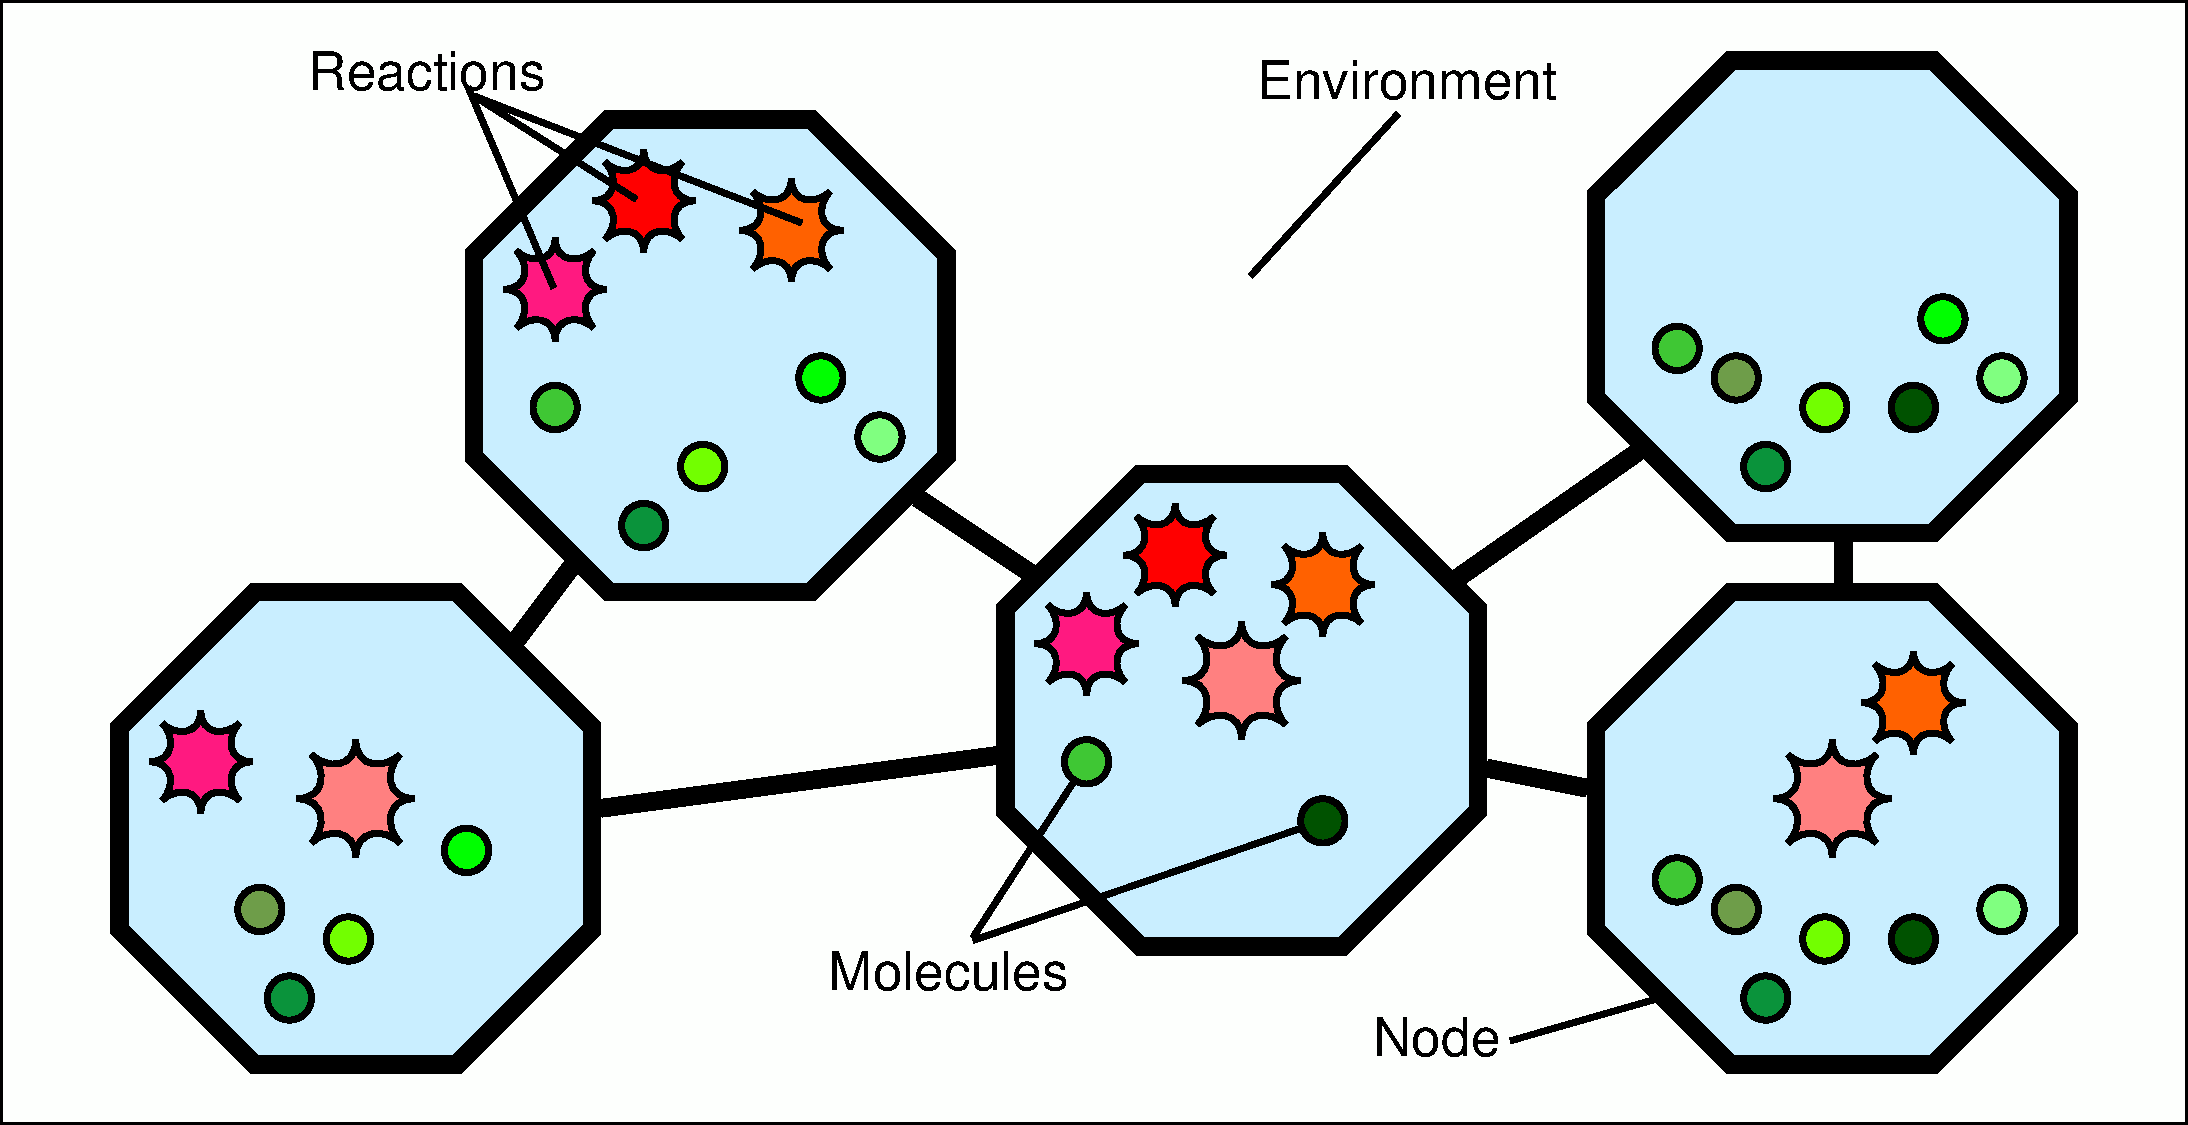
\includegraphics[width=0.99\columnwidth]{img/model.pdf}
    \caption{\alchemist{} computational model: it features a possibly continuous space embedding a linking rule and containing nodes. Each node is programmed with a set of reactions and contains a set of structured molecules.}
    \label{img:model}
  \end{center}
\end{figure}

A pictorial representation of the underlying meta-meta-model is shown in \Cref{img:model}.
%
In this vision of the world, an environment is a multi dimensional space, continuous or discrete, which is able to contain nodes and which is responsible of linking them following a rule.
%
The environment may or not allow nodes to move.
%
Nodes are entities which can be programmed with a set of reactions, possibly changing over time.
%
They also contain molecules, each one equipped with a data structure generalising on the concept of ``concentration''.

\begin{figure*}%[H]
  \begin{center}
    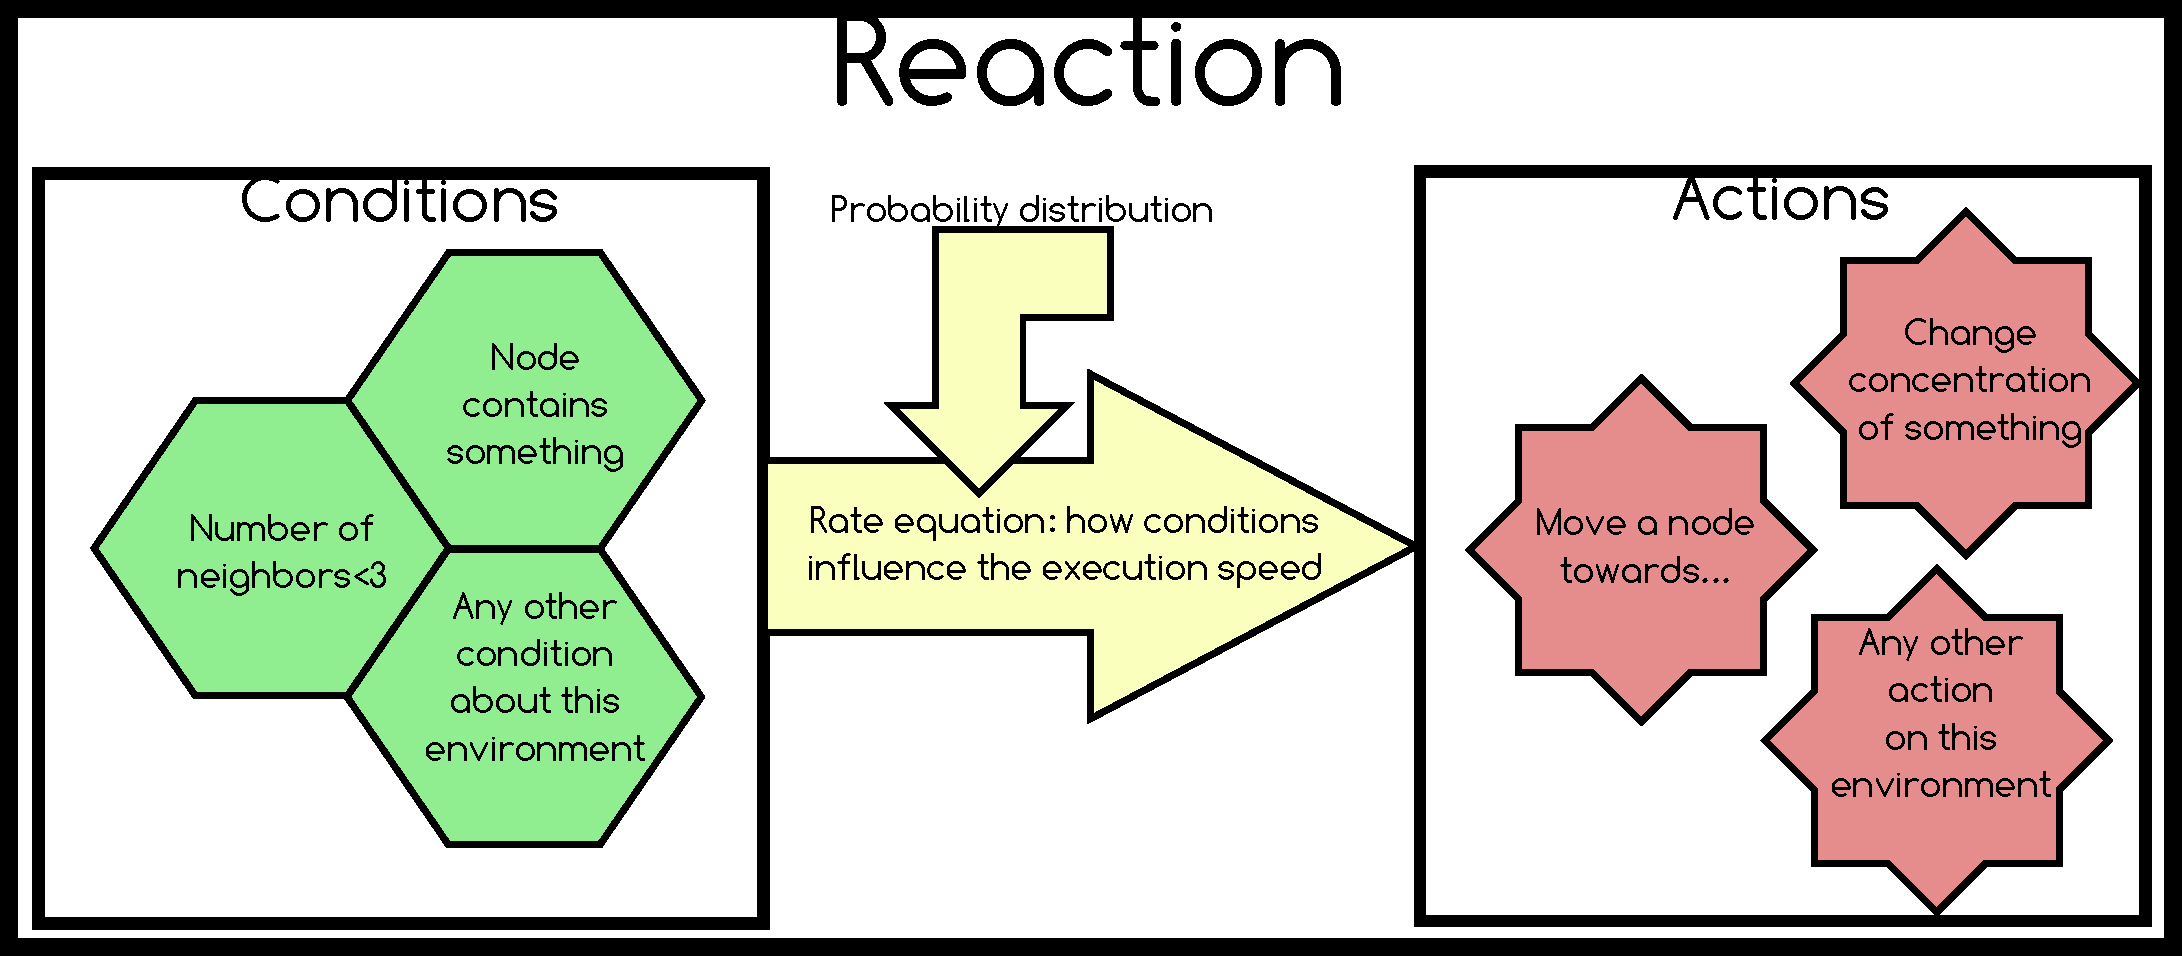
\includegraphics[width=0.99\textwidth]{img/reaction.pdf}
    \caption{\alchemist{} model of reaction: a set of conditions on the environment that determines whether the reaction is executable, a rate equation describing how the speed of the reaction changes in response to environment modifications, a probability distribution for the event and a set of actions, which will be the neat effect of the execution of the reaction.}
    \label{img:reaction}
  \end{center}
\end{figure*}

The concept of reaction is graphically depicted in \Cref{img:reaction}.
%
It allows, for example, to model reactions which are faster if a node has many neighbours, or also reactions that resemble complex biological phenomena such as the diffusion of morphogenes during embryo development as described in \cite{LeccaJIB2010}.
%
It also allows to define which kind of time distribution to use to trigger reactions: this enables us to model and simulate systems based on Continuous Time Markov Chains (CTMCs), to add triggers, or also to rely just on classical discrete time ``ticks''.


\section{Architecture}
%TODO: architettura da rifare

\label{subsec:architecture}
\begin{figure}%[H]
  \begin{center}
    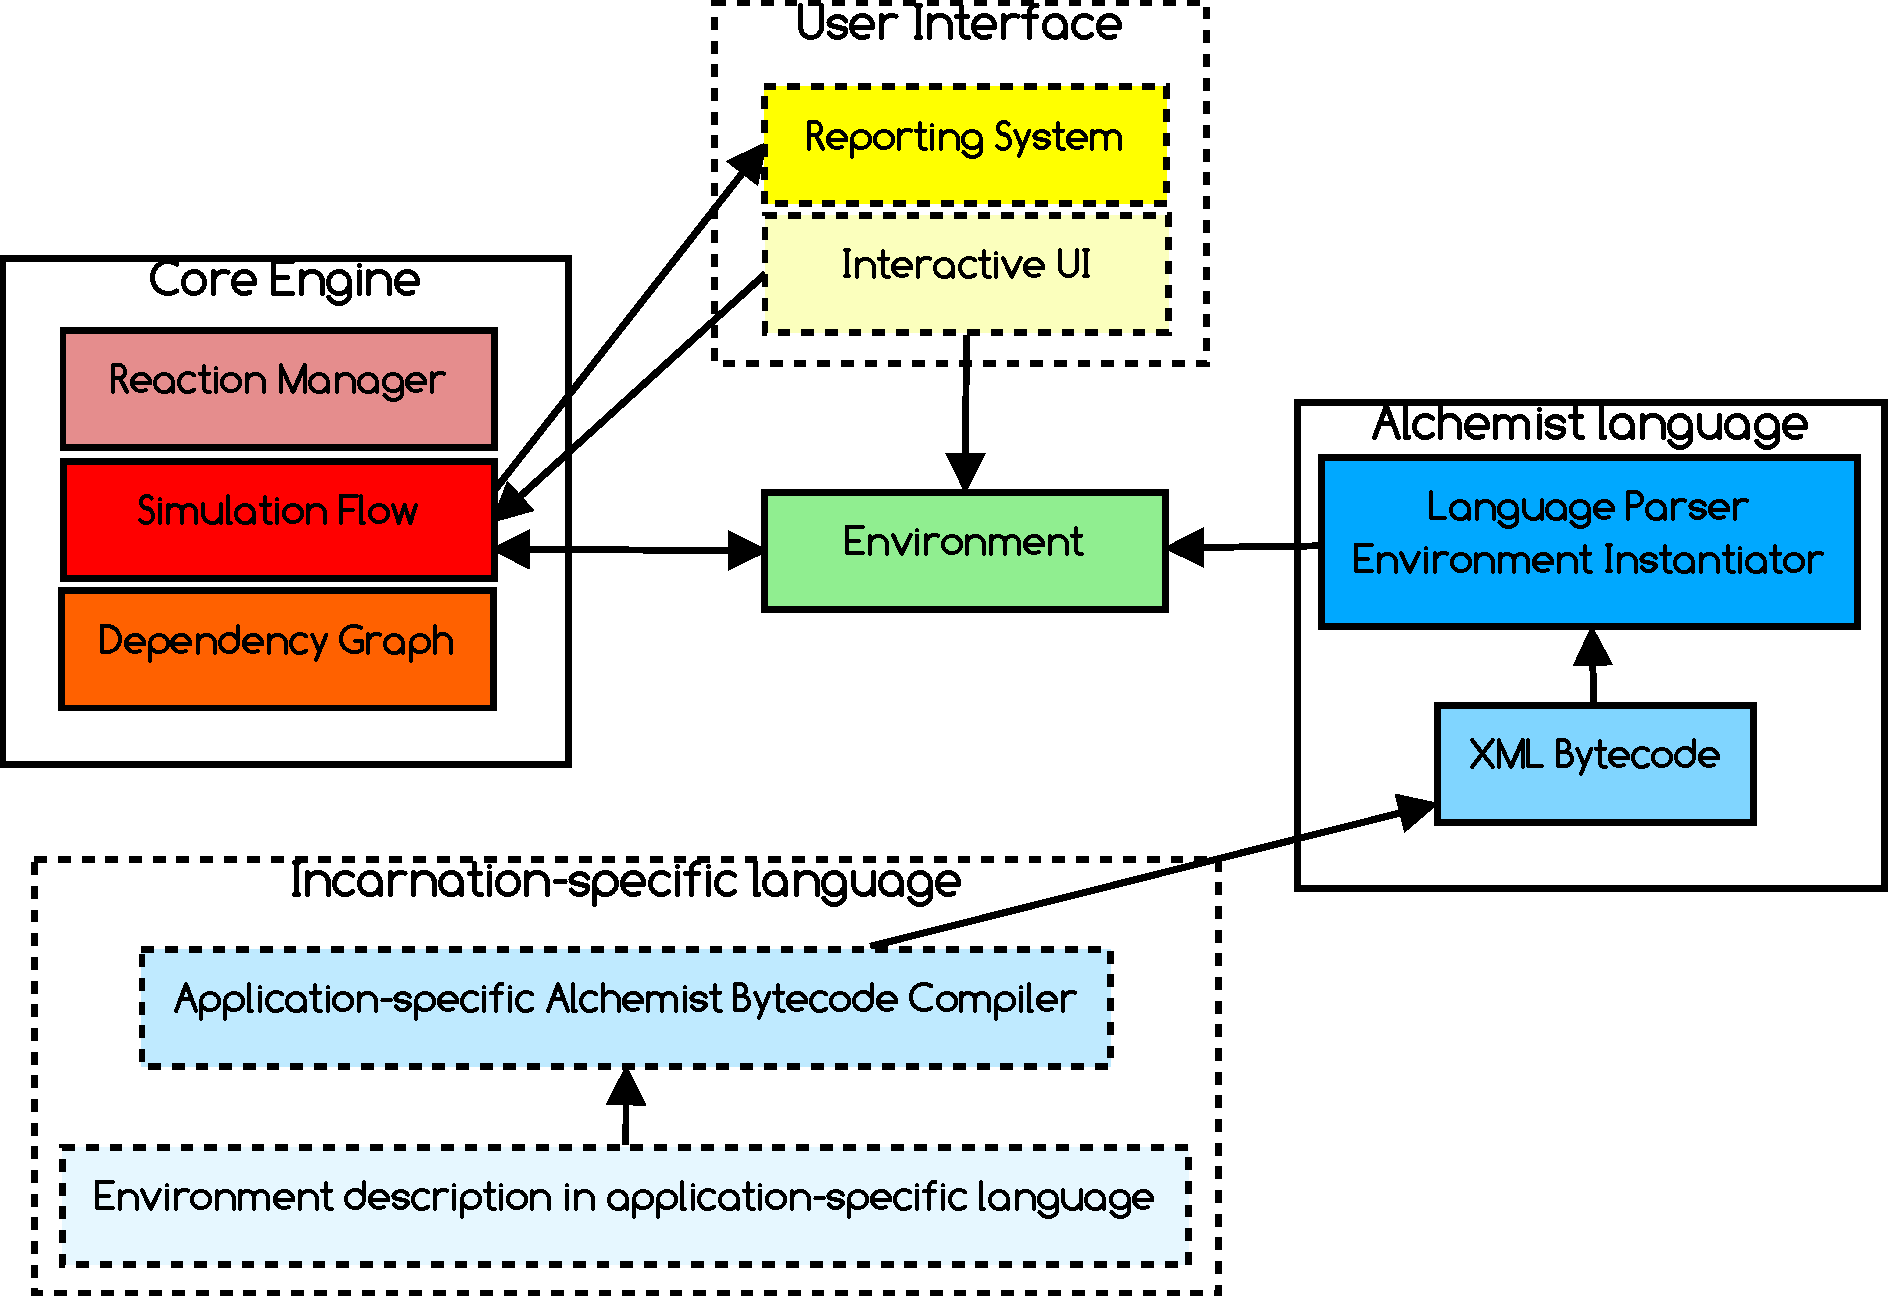
\includegraphics[width=0.99\columnwidth]{img/structure.pdf}
    \caption{\alchemist{} architecture. Elements drawn with continuous lines indicates components common for every scenario and already developed, those with dotted lines are extension-specific components which have to be developed with a specific incarnation in mind.}
    \label{img:arch}
  \end{center}
\end{figure}

The whole framework has been designed to be fully modular and extensible.
The whole engine or parts of it can be re-implemented without touching anything in the model, and on the other hand the model can be extended and modified without affecting the engine.

It is important to note that there is no restriction about the kind of data structure representing the concentration, which can in fact be used to model structured information: by defining a new kind of structure for the concentration, it is possible to incarnate the simulator for different specific uses. For example, by assessing that the concentration is an integer number, representing the number of molecules currently present in a node, \alchemist{} becomes a stochastic simulator for chemistry. A more complex example can be the definition of concentration as a tuple set, and the definition of molecule as tuple template. If we adopt this vision, \alchemist{} can be a simulator for a network of tuple spaces. Each time a new definition of concentration and molecule is made, a new ``incarnation'' of \alchemist{} is automatically defined. For each incarnation, a set of specific actions, conditions, reactions and nodes can be defined, and all the entities already defined for a more generic concentration type can be reused.


%TODO: scrivere una ncarnazione e poi magari anche scrivere una simulazione.

\subsection{Writing a simulation}

%SISTEMARE%

In order to write a simulation, the user must have, or implement herself, an incarnation of \alchemist{}, as described in \Cref{subsec:architecture}.

As shown in \Cref{img:arch}, the simulations are written in a specific XML language containing a complete description of environment and reactions.
%
This code is interpreted in order to produce an instance of an environment: once it is created, no further interpretation is needed in order to run the simulation.
%
This XML code is not meant to be directly exploited by users: the XML format itself is not exactly human friendly, and XML file is often considerably big (a few megabytes are considered to be normal)
%
However, it is a very standard way of describing environments in a machine-friendly format.
%
The idea behind this choice is that \alchemist{} is flexible enough to be used in various contexts, each one requiring a personalised language and a different instantiation of the meta-model.
%
It is up to the extensor to write a translation module from its personalised language to the \alchemist{} XML.
%
Of course, it is also possible to code the simulation behaviour  directly with Java, although this way exposes the user to many more low level details.

\subsection{Implementation details}
%TODO%
The framework was developed from scratch using Java. Being performance a critical issue for simulators, we compared some common languages in order to evaluate their performance level.
%
Surprisingly, Java performance are at same level of compiled languages such as C/C++ \cite{bull2003, oancea2011}.
%
The Java language was consequently chosen because of the excellent trade off between performance, easy portability and maintainability of the code, and the high-level support for concurrent programming at the language level. 
%
The COLT Java library\footnote{\url{http://acs.lbl.gov/software/colt/}} provided us the mathematical functions we needed.
%
In particular, it offers a fast and reliable random number generation algorithm, the so called Mersenne Twister \cite{matsumoto1998}.

% TODO! %
\alchemist{} is still actively developed and currently consists of about 200 classes for about 20'000 lines of code. Though still in beta version, it is released with GPL license as open source \footnote{\mbox{\url{http://alchemist.apice.unibo.it}}.}.

\section{Performance}
\begin{figure}[t]
    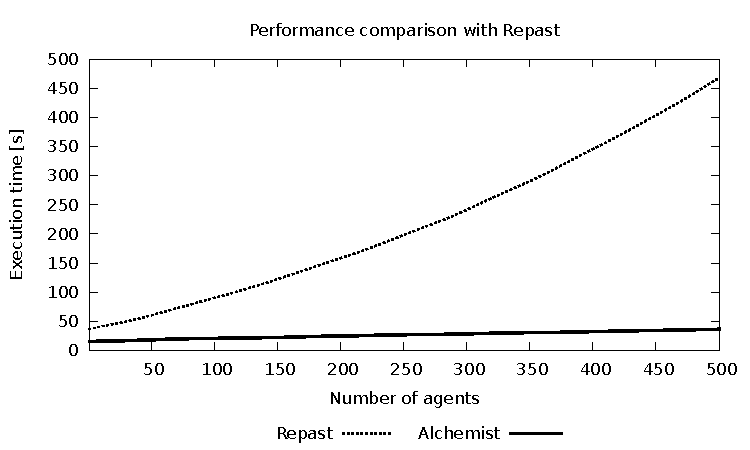
\includegraphics[width=0.999999\columnwidth]{img/jos-graph01}
    \caption{Chart showing the performance scaling of \alchemist{}}
    \label{img:repastperf}
\end{figure}

It is possible to evaluate and compare the performances of \alchemist{} with respect to some known MABS.
%
We exemplify it considering Repast, which we used to developed an alternative simulation for the case study presented in \Cref{jos-museum}\footnote{The source code of the simulation we developed is publicly available at \mbox{\url{http://apice.unibo.it/xwiki/bin/view/Alchemist/JOS/}.}}. There are some important facts that deserve discussion here.

First, since there is no built-in support for stochastic simulation in Repast, we choose to collapse the last five laws of \Cref{img:museum-rules} into a single code path, and the same was made for \alchemist{} by defining a new action.
%
In that way, we were able to avoid for this very specific case the need of a full fledged dependency graph, because there will always be exactly one \textbf{source} and one \textbf{field} per sensor, and no reactions need to be enabled or disabled.
%
This crippled most of the effectiveness of \alchemist{}'s dependency graph, which is indeed a source of optimisation not natively existing in Repast---developing a dependency graph for stochastic simulation in Repast is out of the scope of this thesis, though it would be an interesting subject for future work.
%
On the other hand, it would have been unfair to compare our optimised version against just a plain Gillespie's algorithm built upon Repast.

The second important point is that we choose to encode all the data in both Repast and \alchemist{} as an array of double values instead of real tuples.
%
For \alchemist{}, this meant that we developed a new incarnation for the precise scope of this performance test.
%
The choice of encoding data that way made things faster (no matching required), but also less general.
%
This was done because the SAPERE incarnation of \alchemist{}, which allows us to write the laws as in \Cref{img:museum-rules}, requires a matching system that is not easily portable to Repast.

We choose the configuration of \Cref{img:museum-generalmap2} and we run multiple simulations varying the number of agents per group, in order to evaluate how the two systems scale with the problem size.
%
We measured the running time required to our testbed to run the simulation from the time zero to the time 100.
%
No graphical interface were attached to the simulators while running the batch, in order to evaluate only the raw performance of the engine.
%
The system we used was an Intel Core i5-2500 equipped with 8GB RAM, with Sabayon Linux 7 as operating system and Sun Java HotSpot\texttrademark{} 64-Bit Server version 1.6.0\_26-b03 as Java Virtual Machine.
%
Results are shown in \Cref{img:repastperf}.

Results show the simulator built upon the \alchemist{} framework to be at least twice faster and to scale better than the one built on Repast.
%
Being the dependency graph optimisation cut off as explained above, the reasons for such a difference can lay on the internal scheduler of the engine or in the optimisations in the model.
%
For the first point, we used the default scheduler of Repast Symphony, which is a binary heap implemented through a plain Java array, while our implementation relies on the algorithm and data structures already presented in \Cref{chemical-engine}, so there is not a substantial efficiency difference.
%
For the latter point, a big difference in terms of performances is due to the heavy optimizations of the neighbourhoods of the default \alchemist{} continuous environment.
%
Since the concept of neighbourhood was part of the computational model, it was possible to adopt caching strategies in order to ensure a fast access to the neighbourhood and a quick execution of the operations on it.
%
This is probably the component which gives the highest impact in this case, since most interactions occur among an agent and its neighbourhood.

\section{Collocation in literature}

\subsection{\alchemist{} as a DES}

\alchemist{} is a discrete event simulator (DES), since it combines a continuous time base with the description of system dynamics by distinguished state changes \cite{Zeigler2000}.
%
Since it allows for in-simulation modifications of the environment, it can be considered to belong to the fourth generation of DESs according to \cite{BabulakIJOE2008}.
%
The work in \cite{Pollacia89} surveys the classical DES approaches: according to it, \alchemist{} belongs to the category of simulators featuring ``internal clock'', ``next-event time advance'', and adhering to the ``Event-scheduling World View'', namely, the simulator handles events and is concerned with their effect on system states.

Apart from the meta-model adopted, the main innovative aspect of \alchemist{} with respect to the general DES approach is its ability of optimising the ``compile current event list'' stage \cite{Pollacia89}, which \alchemist{} quickly executes incrementally by means of the management of dependencies that the adoption of a chemical-like model enables.

As far as the simulator model is concerned, instead, the class of DES more related to our approach are those commonly used to simulate biological-like systems.
%
A recent overview of them is available in \cite{EwaldJOS2007}, which takes into account: DEVS \cite{zeigler1984}, Petri Nets \cite{murata1989}, State Charts \cite{Harel1987} and stochastic $\pi$-calculus \cite{Priami1995}.
%
Such an overview however emphasises that all such models require a considerable effort to map biological components into abstractions of the chosen formalism: this is because none of them was specifically developed with biology or bio-inspiration in mind.
%
As described in \Cref{meta-meta-model}, our model is meant to overcome such limitations, since all the enhancements to the basic chemical model we support can be seen as a generalisation of the abstractions of the works presented in \cite{EwaldJOS2007}, and add to them the possibly of customising with much greater flexibility a simulation to the scenarios of bio-inspired computational systems.

We should finally note that the DES approach typically contrasts the use of mathematical techniques (e.g. modelling the system by differential equations).
%
However, the possible different choice of translating a system model to ordinary or partial different equations -- which can be solved numerically in a time considerably shorter than a set of stochastic simulations -- is shown to be impractical in our case.
%
This path, explored for example by \cite{MallavarapuInterface2008}, can provide good results for dynamics that progress at more or less the same speed, and in which abundance of species (data-items or agents in our case) is so high that it can be relaxed to real-valued variables \cite{EwaldJOS2007}.
%
This is not the case for many scenarios even in system biology (see, for example, \cite{Cowan2000, UhrmacherWSC2005}), not to mention scenarios like pervasive computing where reaction rates do not change continuously, and where the effect on an even small number of agents can be key to a given system evolution.

\subsection{\alchemist{} as a MABS}

Even though chemical-inspired, the meta-meta-model described in \Cref{meta-meta-model} holds evident relationships with multi-agent-based simulation (MABS) approaches.

According to \cite{BandiniJASSS2009}, agent-based platforms for simulations can be split in three categories: general purpose frameworks with specific languages (such as NetLogo), general purpose frameworks based on general purpose programming languages (such as Repast \cite{repast}) and frameworks which provide an higher level linguistic support, often targeted to a very specific application (e.g. \cite{WeynsAAMAS2006}).
%
Each approach has clearly its own advantages and weaknesses.
%
Usually, the more general purpose is the language, the wider is the set of possible scenarios, and the wider is also the gap between the language and the simulated model.
%
This means that an higher level language allows the user to create and tune its simulations in an easier way, on the other hand it often restricts the generality of the tool. 

\alchemist{} is meant to provide a set of meta-models, possibly each with its own domain specific language, still maintaining the possibility to extend or re-implement certain abstractions using the general purpose Java language (defining a new ``incarnation'', namely a new meta-model).

\subsubsection{Advantages}

There is a set of applications which are better tackled by \alchemist{}.
%
In particular, \alchemist{} is suitable for all those simulation scenarios in which agents have relatively simple behaviour, and the notion of agent-based environment plays instead a fundamental role in organising and regulating the agents' activities \cite{BandiniE4MAS2006} by both enabling local interactions among the proactive entities \cite{HellebooghAAMAS2007} and enforcing coordination rules \cite{aose-mags5}, allowing the modeller to shift her focus from the local behaviour of the single agent to a more objective vision of the whole MAS \cite{SchumacherCEEMAS2007}. 
%
The idea of dealing with a strong notion of environment in multi-agent systems has been deeply developed in a series of work: other than its importance in the simulation context \cite{HellebooghAAMAS2007}, at the infrastructure level \cite{VHRSZ-JAAMAS2007} and at the methodological level \cite{aose-mags5}, there have been proposals of meta-models such as A\&A \cite{artifacts-jaamas17} and infrastructures such as \tucson{} \cite{tucson-aamas99} and \cartago{} \cite{RPV-JAAMAS2011}.
%
A common viewpoint of all these works is that the behaviour of those passive and reactive components structuring the environment (e.g. \emph{artifacts} in A\&A) is well defined in terms of rules expressed as declarative conditions-imply-actions fashion.
%
Accordingly, \alchemist{} is particularly useful either in computing systems following the chemical inspiration \cite{VCMZ-TAAS2011,VZ-INS2010,sapere-procedia7}, or for agent-oriented systems where the role of the environment is key, up to be a very dynamic part of the whole system---where network nodes (or, in biological terms, compartments) can move, new nodes can be spawn or be removed from the system, and links can appear or break at runtime as happen e.g. in pervasive computing scenarios \cite{sapere-procedia7}.

\subsubsection{Limitations}

Inevitably, as an attempt to build a hybrid between agent-based simulators and (bio)chemical simulators, some trade-offs had to be accepted, which ultimately makes \alchemist{} less suited for certain classes of applications.
%
In particular, a limitation is that \alchemist{}'s agent actions have to be mapped onto the concept of reaction. 
%
On the one hand, this makes it rather straightforward to create reactive memoryless agents \cite{BandiniJASSS2009}, whose goal is just to perform rather easy computations resulting in the creation, deletion or modification of information items in the environment.
%
In fact, since it is allowed to program different nodes with different reactions, it is easy to code reactive and context-dependent agents. On the other hand, there is neither out-of-the-box facility nor any high level abstraction useful to define intelligent agents \cite{BandiniJASSS2009}. The simulator is able to run them provided the user manually writes their whole behaviour as a single Java-written reaction---and properly specifies dependencies with other reactions.
%
Although possible in principle, performing this task too frequently is likely breaking the \alchemist{} abstraction, making the programmer losing the nice declarative approach that chemistry endorses, and possibly hampering the optimisation techniques that motivated \alchemist{}.

\section{Meta-model agnostic features}

This section analyses the main features of \alchemist{} that can be exploited regardless the specific ``incarnation''.
%
They add a great value to the tool, since they can be used immediately after the creation of a novel meta-model, with no need to specifically write any new code besides some minimal glue.

\subsection{Distributed statistical analysis}

As we have seen in \Cref{engineering-and-tools}, simulation represents a key step in the engineering of pervasive systems.
%
Being a simulation basically a sampling over an enormous probability space, obvious questions accompany these procedures:
\begin{itemize}
 \item how reliable are the obtained values?
 \item How is the number of performed simulations chosen?
 \item How many simulations are required in order to state system properties with a certain degree of confidence?
\end{itemize}

Moreover, there is frequently a lack of decoupling between the model specification and the definition of the system's properties of interest: they are often embedded in the model, and their values are obtained via logging operations performed during the simulation process.

This section presents a tool meant to face these challenges, obtained chaining \alchemist{}, with \multivesta{}\footnote{\url{http://code.google.com/p/multivesta/}} \cite{multivesta}, a recently proposed lightweight tool extending \vesta{}~\cite{Sen:2005} and \pvesta{}~\cite{AlTurkiM11} which allows to enrich existing discrete event simulators with automated and distributed statistical analysis capabilities.
%
The result is thus a statistical analysis tool tailored to chemical-inspired pervasive systems.
%
The benefits obtained by chaining the simulator with \multivesta{} are:
\begin{enumerate}
 \item a language (\multiquatex) to compactly and cleanly express systems properties, decoupled from the model specification;
 \item the automated estimation of the expected values of \multiquatex{} expressions with respect to \emph{n} independent simulations, with \emph{n} large enough to respect a user-specified confidence interval;
 \item an interactive plot as well as the generation of gnuplot input files to visualize the obtained results;
 \item a client-server architecture to distribute simulations.
\end{enumerate}

\multivesta{} is independent on the model specification language: it only assumes that discrete event simulations can be performed on the input model.
%
As described in~\cite{multivesta}, the tool offers a clean interface to integrate existing discrete event simulators, enriching them with a property specification language, and with efficient distributed statistical analysis capabilities.

\subsubsection{\multivesta{} and \multiquatex{}}

\multivesta{} performs a statistical (Monte Carlo based) evaluation of \multiquatex{} expressions, allowing to query about expected values of observations performed on simulations of probabilistic models. 
%
A \multiquatex{} expression may regard more measures of a model, in which case the same simulations are reused to estimate them, thus improving the performance of the analysis tasks. %
Moreover, the tool has a client-server architecture allowing to distribute the simulations on different machines.
%
A detailed description of \multiquatex{} and of the procedure to estimate its expressions is out of the focus of this work, the interested reader can deepen her knowledge reading \cite{multivesta,AghaMS06}.
%
Before defining a \multiquatex{} expression, it is necessary to specify the state characteristics to be observed.
%
This model-specific step ``connects'' \multiquatex{} with the model.
%
The state observations are offered via the \texttt{{rval}}(\emph{obs}) predicate which returns a real number for each observation, specified by the string parameter \emph{obs}. 

A \multiquatex{} expression consists of a set of definitions of \emph{parametric recursive temporal operators}, followed by a list of \emph{\texttt{eval} clauses}. Each \texttt{eval} clause relies on the defined temporal operators, and specifies a property whose expected value must be evaluated.

In order to evaluate a \multiquatex{} expression, \multivesta{} performs several simulations, obtaining from each a list of samples (real numbers).
%
One sample for each \texttt{eval} clause is obtained, thus all the queried measures are evaluated using the same simulations, improving performance.
%
Based on the samples obtained from simulations, \multivesta{} estimates \multiquatex{} expressions with respect to two user-provided parameters: $\alpha$ and $\delta$. 
%
Considering the case of simple expressions with just one \texttt{eval} clause, the estimations are computed as the mean value of the $n$ samples obtained from $n$ simulations, with $n$ large enough to grant that the size of the $(1 - \alpha)*100\%$  \textit{Confidence Interval} (CI) is bounded by $\delta$.
%
In other words, if a simple \multiquatex{} expression is estimated as $\overline{x}$, then, with probability $(1 - \alpha)$, its actual expected value belongs to the interval $[\overline{x} - \delta/2,\overline{x} + \delta/2]$.
%
The case of expressions with multiple \texttt{eval} clauses is similar, with the note that the \texttt{eval} clauses may regard values of different orders of magnitude, and thus the user may provide a list of $\delta$ rather than just one. 
%
After having obtained a sample for every \texttt{eval} clause from a simulation, these values are used to update the means of the samples obtained from previous simulations (one mean per \texttt{eval} clause). If the CIs have been reached for every \texttt{eval} clause, the evaluation of the expression is terminated, otherwise further simulations are performed.
%
Note that each \texttt{eval} clause may require a different number of simulations to reach the required CI. Once the CI of an \texttt{eval} clause has been reached, such \texttt{eval} clause is ignored in eventual further simulations performed for other \texttt{eval} clauses. 


\subsubsection{Integrating \multivesta{} and \alchemist{}}

In order to chain the tools, some steps, have been tackled once and for all, while others are model-specific.
%
Essentially, in order to allow the interaction with \multivesta{}, \alchemist{} has to fulfill two requirements:
\begin{enumerate}
 \item the ability to advance the simulation in a step-by-step manner (which is provided by the \texttt{playSingleStepAndWait} method in \texttt{ISimulation} interface);
 \item the ability to analyze the model status after each simulation step, providing measures in form of real numbers about properties of interest.
\end{enumerate}

Since both \multivesta{} and \alchemist{} are Java-based, their interaction has been easily realized by subclassing the \texttt{NewState} class of \multivesta{}.
%
The obtained \texttt{AlchemistState} class is sketched in \Cref{lst:alchemiststate}, where unnecessary details are omitted.
The new class contains some \alchemist{}-specific code, providing \multivesta{} with the simulation control and proper entry points for the analysis.

\begin{lstlisting}[frame=single, basicstyle=\scriptsize, language=Java, mathescape, caption=AlchemistState extending \multivesta{}'s NewState class, label=lst:alchemiststate,float=t,numbers=left]
public class AlchemistState<N extends Number, D extends Number, T> extends NewState {
  private final long maxS; 
  private final ITime maxT;
  private ISimulation<N, D, T> sim;
  ...
  public AlchemistState(final ParametersForState params) throws ...{
    super(params);
    final StringTokenizer otherparams = new StringTokenizer(params.getOtherParameters());
  /* Initialization of Alchemist-specific parameters
     and execution environment resorting to otherParams */
  }
  ...
  public void setSimulatorForNewSimulation(final int seed) {
    /* Stop current simulation, create a new one. */
    ...
    sim.stop();
    ...
    env = getFreshEnvironment(seed);
    sim = new Simulation<>(env, maxS, maxT);
    ...
  }
  ...
  public void performOneStepOfSimulation() {
    sim.playSingleStepAndWait();
  }
  ...
  public double rval(final String obs) {
    if(obs.equals("time")) return getTime();
    if(obs.equals("steps")) return getStep();
    //other model-independent observations 
    ...
    return getStateEvaluator().getVal(obs, this);
  }
}
\end{lstlisting}

In the constructor (lines $6$-$10$), the superclass initialization is done by a simple \texttt{super()} call.
%
The remaining code initializes \alchemist{}-specific parameters such as the maximum time or steps to simulate.
%
Those  are in general not required, since \multivesta{} is able to detect when the analysis requirements have been met, and consequently stop the simulation flow.
%
The method \texttt{setSimulatorForNewSimulation()} is depicted in lines $12$-$20$.
%
The method is invoked by \multivesta{} before performing a new simulation to (re)initialize the status of the simulator, providing to it a new random seed. 
%
In lines $22$-$24$, \texttt{performOneStepOfSimulation()} is provided: resorting to the \alchemist{} method \texttt{playSingleStepAndWait()}, it allows \multivesta{} to order the execution of a single simulation step.

In order to inspect the simulation state, the \texttt{rval()} method defined in lines $26$-$32$ is invoked.
%
The argument specifies the observations of interest.
%
This method inspects the simulation state for all aspects common to any \alchemist{} model, e.g., in the listing are sketched the current simulated time (line $27$) and the number of performed simulation steps (line $28$).
%
Clearly, each \alchemist{} model will have its own observations of interest.

Depending on the model at hand, it may be necessary to refine the model-independent observations exposed by \texttt{AlchemistState} with a set of model-specific ones. This can be done by simply instantiating the \texttt{IStateEvaluator} interface provided by \multivesta, constituted by one method only.

\subsubsection{Example}

This section discusses the analysis performed on a crowd steering scenario, similar to the one which will be presented in detail in \Cref{jos-museum}.
%
In such scenario, two group of people are inside an indoor environment, and are steered towards two point of interest (POI) such that their ideal trajectory intersect, creating a crowd.
%
The steering system is implemented leveraging the SAPERE meta-model, and as such data items in this scenario are called \texttt{LSA}s.
%
This example is not meant to provide significant scientific insights on crowd steering (thoughts about it will be provided in the remainder of this thesis), but rather to act as toy-example to demonstrate the flexibility and possibilities of the chaining of \alchemist{} and \multivesta{}.

The outcome of the analysis is summarized in the three charts of \Cref{img:analysisCharts} (obtained using the gnuplot input files provided by \multivesta{}), showing, at the varying of the simulated time, the expected values of: the number of people which have reached their point of interest (top), the average number of connections of the devices (middle), and the number of LSAs in the system (bottom).

\lstset{caption=The evaluated parametric multi-expression ($MainMQ$), label=listing:parametricMQ}
\begin{lstlisting}[frame=single, mathescape, morekeywords={parametric,eval,E,if,fi,then,else,s,rval,evalME,evalOnceME}, float=t, numbers=left]
people@POI($x$) = if{s.rval("time") >= $x$}
      then s.rval("bPOI")
      else $\textbf{{\#}}$people@POI($x$)
   fi;
people@RPOI($x$) = // similar to people@POI
people@LPOI($x$) = // similar to people@POI
avgConn($x$) = if{s.rval("time") >= $x$}
      then s.rval("degree")
      else $\textbf{{\#}}$avgConn($x$)
   fi;
LSAs($x$) = if{s.rval("time") >= $x$}
      then s.rval("LSAs") 
      else $\textbf{{\#}}$LSAs($x$)
fi;
eval parametric(E[people@POI($x$)],E[people@RPOI($x$)],              E[people@LPOI($x$)],E[avgConn($x$)],E[LSAs($x$)],$x$,$0.0$,$1.0$,$50.0$);
\end{lstlisting}

The three charts have been obtained by evaluating $MainMQ$ of \Cref{listing:parametricMQ}, having $5$ parametric temporal operators (lines $1$-$9$):
%
\texttt{people@RPOI} and \texttt{people@LPOI} regard the number of people which have reached, respectively, the POI on the right and the one on the left, while \texttt{people@POI} counts instead how many people have reached their destination. The fourth temporal operator (\texttt{avgConn}) regards the connectivity degree of the devices. Finally, \texttt{LSA}s regards the number of LSA in the system, giving insights on the amount of memory required to sustain the system.
%
The temporal operators are analysed at the varying of the simulated time from $0$ to $50$ seconds, with step $1$ (line $10$). Thus the analysis consisted in the estimation of the expected values of the $5$ temporal operators instantiated with $50$ parameters, for a total of $250$ expected values. 

\begin{figure}
\begin{center}
\vspace{-0.2cm}
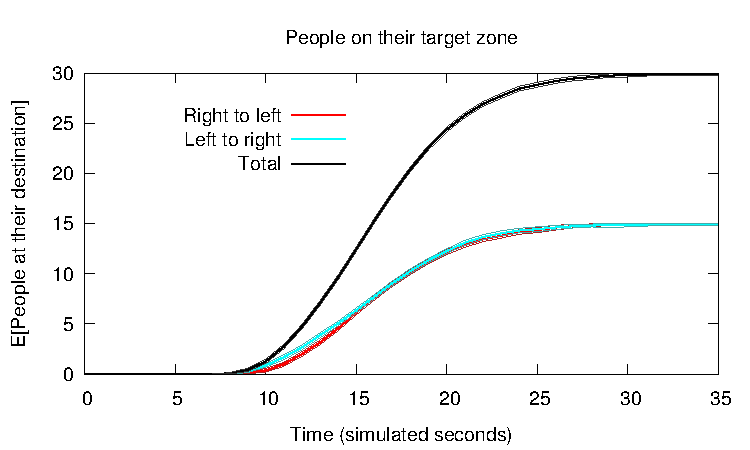
\includegraphics[width=0.7\columnwidth]{img/people}
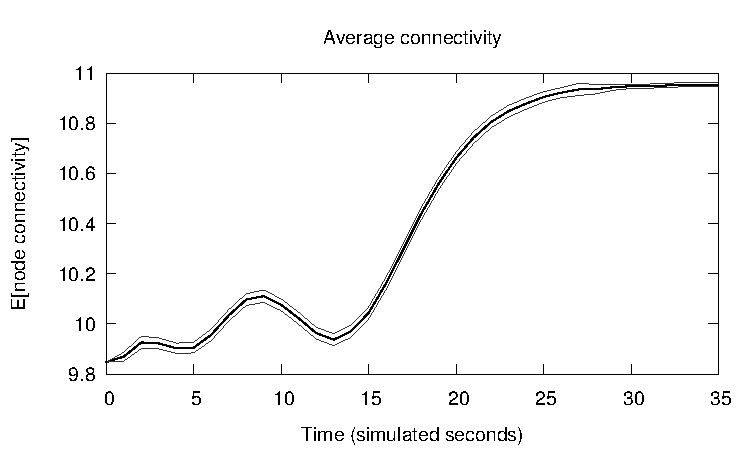
\includegraphics[width=0.7\columnwidth]{img/connectivity}
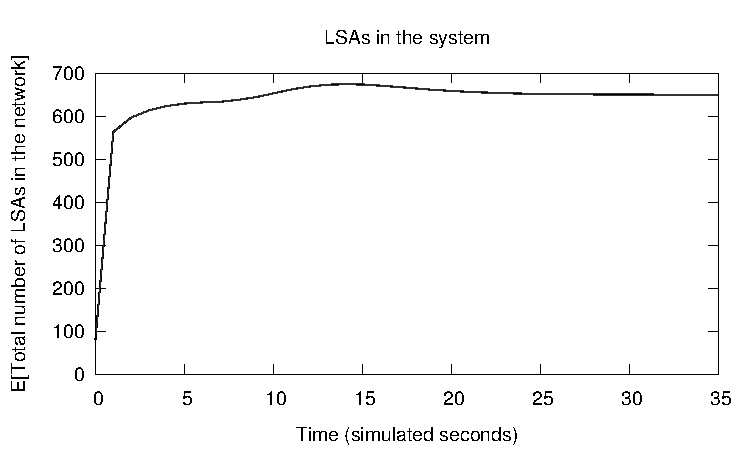
\includegraphics[width=0.7\columnwidth]{img/lsas}
\caption{Analysis of the crowd steering scenario: (top) number of people at the POIs, (middle) average number of connections per device, (bottom) number of LSAs in the system.}
\label{img:analysisCharts}
\end{center}
\end{figure}

A high degree of precision has been required: $\alpha$ has been set to $0.01$, while the $\delta$ values (the size of the CIs) have been chosen considering the orders of magnitude of the measures: $0.5$ for the instances of \texttt{people@POI($x$)}, \texttt{people@RPOI($x$)} and \texttt{people@LPOI($x$)}; $0.05$ for  \texttt{avgConn($x$)}; and $3$ for \texttt{LSAs($x$)}.
%
To reach such a level of confidence, the tool ran approximately $2500$ simulations, requiring less than a hour.
%
The discussed confidence intervals are depicted in the aforementioned charts: the two lines drawn above and below the central lines represent the obtained CIs of the expected values, thus indicating the intervals in which the actual expected values lie with probability $0.99$.

The top chart regards the first $3$ temporal operators: the top plot refers to the number of people in total which have reached their target POI, while the two almost over-imposed lower plots regard the number of people at the right POI and at the left POI. 
%
All the three measures under analysis produced monotonically increasing sigmoid curves.
%
We can deduce from this behavior that there are no systemic errors in the crowd steering system, such as people with no or wrong suggested final destination, in which case we would have noticed one or more flatted zones flawing the sigmoid curve.
%
We note also that after around 30 simulated seconds all the people have reached their target, and that it takes around 10 seconds for the fastest walkers to get to their destination.
Note that, despite that the analysis has been performed for 50 simulated seconds, the charts presented in \Cref{img:analysisCharts} have been cut at time 35 to better show the most relevant results: in fact, the system reaches stability after this time, and no event of interest happens later.
%
Moreover we can also notice that people going from left to right are slightly faster than the other group.
%
This difference, due to the asymmetric positioning of people in the center of the scenario, is hardly visible and would have been impossible to spot with a lower precision analysis.

The middle chart shows the evolution in time of the average number of connections of the devices (i.e., both sensors and smartphones).
%
Since each device is considered to be connected to all those within a range of 1.5 meters, it also gives us a hint about the crowding level.
%
There is a noticeable peak at around 8 seconds: it is due to a high number of people approaching the central group.
%
After that, the peak disappears when most people overtook the obstacle and are walking towards their POI.
%
Finally, there is a growth: progressively, people reach their destination and tend to create a crowd.

The bottom chart shows the number of LSAs in the whole system, indirectly giving hints on the global memory usage.
%
Once the system is started, there is a very quick growth, due to the gradient being spread from the sources to the whole sensors network and to the LSAs produced by the crowd-sensing.
%
The system reaches a substantial stability after a couple of seconds.
%
From that point on, the number of LSAs has very little variations: the system has no ``memory leak'', in the sense that it does not keep on producing new LSAs without properly removing old data. 

\subsubsection{Performance Assessment}
All the experiments of the previous section have been run on a machine equipped with four Intel\textregistered{} Xeon\textregistered{} E7540 and 64GB of RAM, running Linux 2.6.32 and Java 1.7.0\_04-b20 64bit.

In order to measure the performance scaling of the tool, we ran our analysis multiple times varying the number of \multivesta{} servers deployed.
%
Results are summarized by the dark line of \Cref{img:performance}, showing that with only 1 server (\alchemist{} does not have any parallel capability by its own), the analysis required almost 17 hours, while with more than 30 servers (enabled by the chaining with \multivesta{}) it required less than an hour. For the considered scenario, by distributing simulations we have thus obtained a more than eighteen times faster analysis.

\begin{figure}[t]
\begin{center}
\vspace{-0.2cm}
%  \includegraphics[width=0.49\textwidth]{charts/perfcomp}
 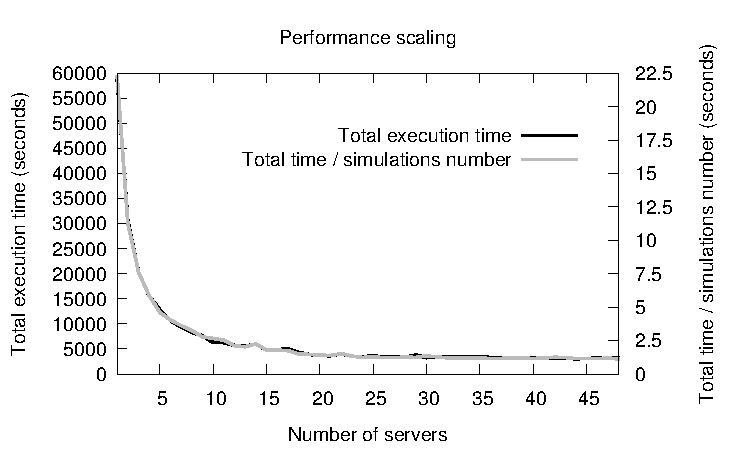
\includegraphics[width=0.99\textwidth]{img/scaling}
 \end{center}
%  \caption{Performance improvement reusing simulations (left), performance scaling a the varying of the number of used cores (right).}
 \caption{Performance scaling with of the number of running servers.}
 \label{img:performance}
\end{figure}

It is worth to note that such comparison of performance is affected by the statistical nature of the analysis procedure. 
%
Intuitively, when evaluating a \multiquatex{} expression resorting to $x$ or to $x + y$ servers, in both cases we initialize the first $x$ servers with the same $x$ seeds, generating thus the same $x$ simulations. However, the remaining $y$ servers are initialized with new seeds, and thus produce new simulations.
Clearly, by having different simulations, we may obtain different sample variances, requiring a different number of simulations.
%
For this reason, the bright line of \Cref{img:performance} depicts the time analysis normalized with respect to the number of simulations (obtained dividing the overall analysis time by the number of performed simulations).
%
The two lines of \Cref{img:performance} evolve accordingly, thus confirming the great performance gain brought by the distribution of simulations.

\begin{table}[tb]
 \caption{Time performance improvements reusing simulations (seconds).}
%\begin{figure}[t]
%\caption{{Performance improvements reusing simulations. Times are in seconds.}}
\begin{center}
\scalebox{0.82}{
 \begin{tabular}{| c | c | c | c |}
 \hline
 %\hline
 & \textbf{Expressions} & \textbf{Param. expressions} & \textbf{Param. multi-expressions} \\
 \hline%\hline
 \textbf{\texttt{people@POI}} & 
 %THIS IS THE CORRECT NUMBER { 28045.77}
 28045.77
 %39999.32 %IN THE PAPER SUBMITTED TO 4PAD WE DISCUSSED THIS 
 & 2567.26 & n.a. \\
 \hline
 \textbf{\texttt{people@RPOI}} & 15891.13 & 1114.86 & n.a. \\
 \hline
 \textbf{\texttt{people@LPOI}} & 15560.83 & 950.30 & n.a. \\
 \hline
 \textbf{\texttt{avgConn}} & {%\color{blue}
 90111.29}  % 
 & 1372.64 & n.a. \\
 \hline
 \textbf{\texttt{LSAs}} & 58630.45 %1m11.231 
 & 2504.33 & n.a. \\
 \hline\hline
 \textbf{Total time} & {%\color{blue}
 %220193.02
  208239.47
 } & 8509.39 & 3215.95 \\
 \hline
 %\hline
 \end{tabular}}
\end{center}
 %\caption{Time performance improvements reusing simulations (seconds).}
 \label{tab:reuse}
%\end{figure}
\end{table}

\multivesta{} has a further important feature which dramatically reduces the analysis time: the reuse of simulations to estimate many expected values. 
%
The reusage happens on two levels:
\begin{enumerate}
 \item expressions can be made parametric, and thus simulations can be reused for computing the same property at the varying of a parameter (e.g., at different time steps);
 \item it is possible to write multi-expressions , and thus reuse simulations to evaluate multiple properties.
\end{enumerate}
%
Moreover,  by combining these two features, it is possible to reuse simulations for multiple parametric properties (e.g. $MainMQ$ of \Cref{listing:parametricMQ}).
%
As explicated by \Cref{tab:reuse} (whose reported analysis have been performed resorting to 48 servers), 	parametric expressions (second column) allowed us to save a stunning {%\color{blue}
96}\% of execution time with respect to the simple expressions case without reuse of simulations (first column). Moreover, the parametric multi-expression feature (third column) allowed us to further cut down this time to a third.
%
We can thus advocate that, by exploiting reuse of simulations, for the considered scenario we obtained a more than 64 times faster analysis.
%
Clearly, the performance gains change depending on the considered scenario or properties. In fact, the more simulations are required, and the longer they take, the greater will be the advantage.

\subsection{Real world maps}

\alchemist{} supports real-world environments.
%
The base functionality lies in the possibility to load maps and simulate within them.
%
Currently, the simulator supports OpenStreetMap\cite{osm}, and it is able to load data in multiple OSM XML, compressed OSM XML and Protcolbuffer Binary Format (PBF).
%
The latter is warmly recommended for both performance and map file size.
%
Various websites provide ready-to-use extracts of the world map in PBF format for cities and whole regions, and arbitrarily sized extracts in OSM XML format can be obtained via public web API.

Once the map has been loaded, \alchemist{} offers the possibility to enrich the simulations with the maps data, and in particular offers various ways to move nodes within the environment taking into account the characteristics of the map.

The first feature offered is about the initial node displacing.
%
When adding a node to the environment, in fact, it is possible not to displace the node in the exact position indicated, but in the nearest street point.
%
This comes in particularly handy in order to realise the network of static devices: the simulator can be fed with a grid of devices, and it automatically modifies the positions of each node in order to displace it on a street.

 \begin{figure}
  \subfigure[GPS trace]{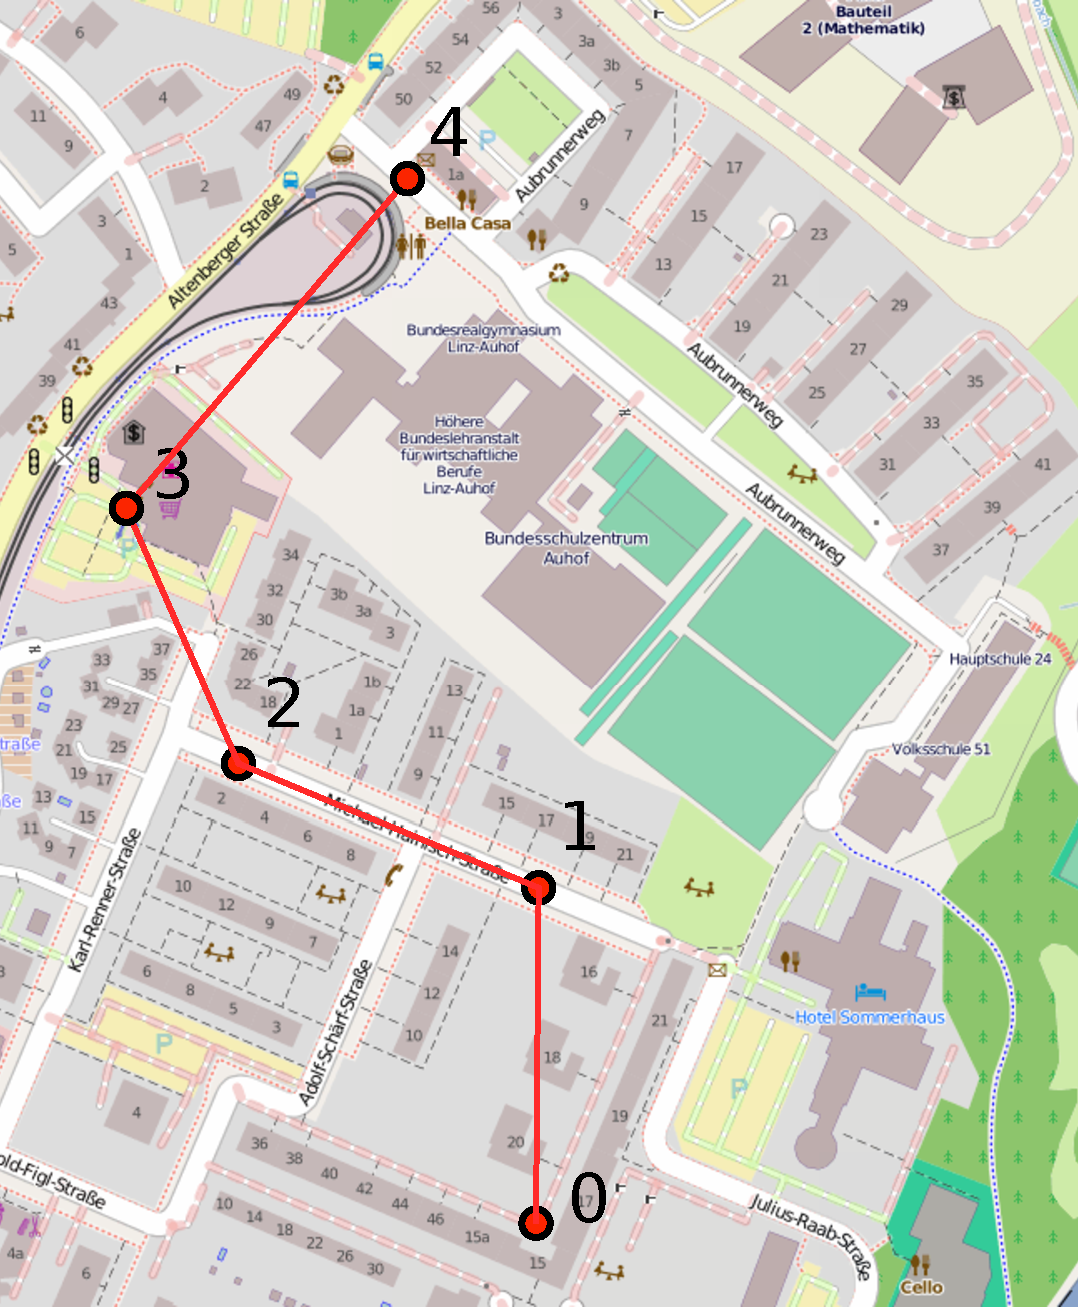
\includegraphics[width=0.315\textwidth]{img/gps}
   \label{img:gps-alchemist-navi}
  }
~
  \subfigure[Map-based navigation]{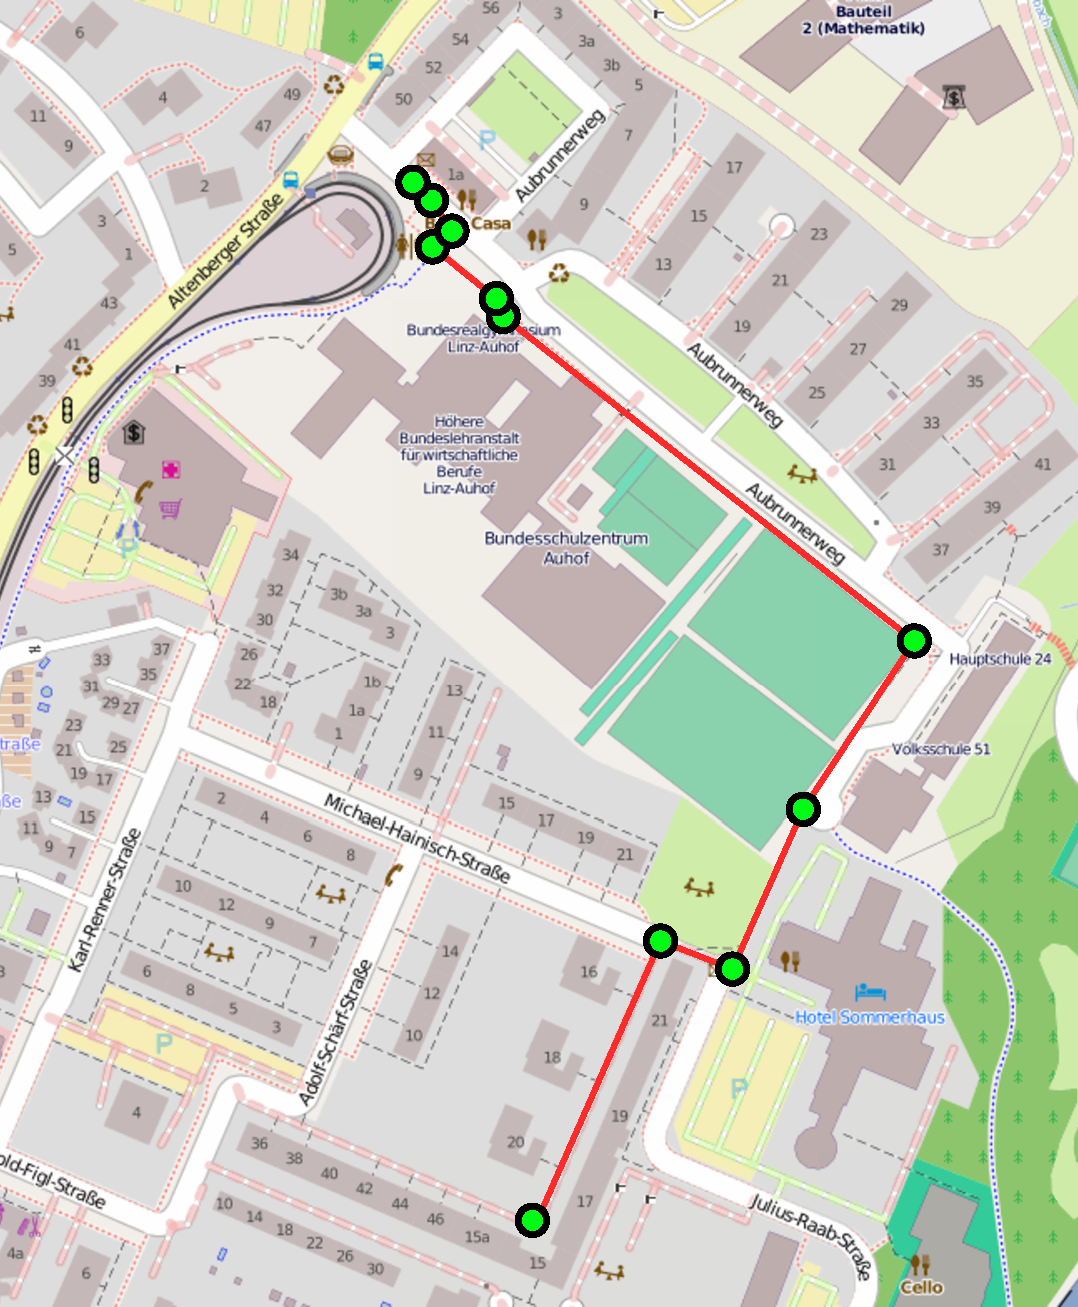
\includegraphics[width=0.315\textwidth]{img/map}
   \label{img:map-alchemist-navi}
  }
~
  \subfigure[Mixed mode]{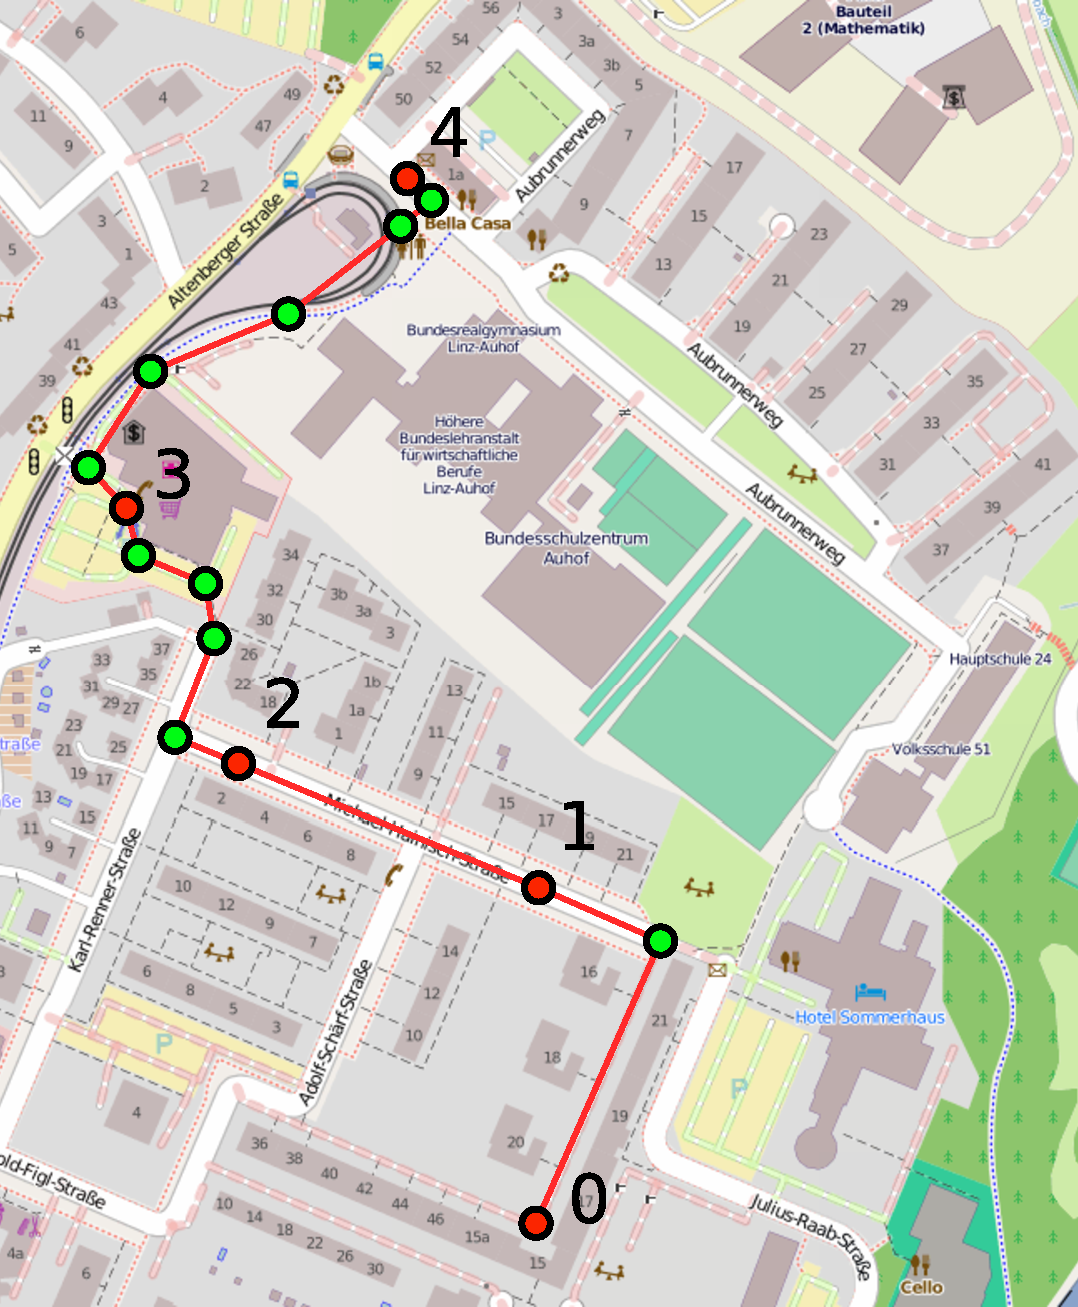
\includegraphics[width=0.315\textwidth]{img/mixed}
   \label{img:mixed-alchemist-navi}
  }
 \caption{Three snapshots showing the different navigation modes available in \alchemist{}. In \Cref{img:gps-alchemist-navi} there is a GPS trace consisting in four points. If not specified to behave otherwise, \alchemist{} computes the average speed between two points, and moves the node along a straight line with constant speed. This, depending on the precision of the trace, may generate paths that cross over buildings. In \Cref{img:map-alchemist-navi}, the route between the start and end point is computed using the built-in navigator. This could lead the nodes towards paths different from those described by the route. In \Cref{img:mixed-alchemist-navi}, the routing subsystem is used to refine the quality of the GPS traces: \alchemist{} will move the node with constant speed between the two points, using map based routing when necessary to improve precision between two consecutive trace points.}
 \label{img:traces-navigation}
\end{figure}



The second useful feature is the possibility to rely on the map data to compute routes, as in \Cref{img:map-alchemist-navi}.
%
\alchemist{} in fact ships with a module based on GraphHopper \footnote{\url{http://graphhopper.com/}} which provides the simulator the ability to compute routes between two points of the map.
%
This feature is mainly used to steer nodes correctly along the map, following the allowed ways.
%
It is possible to use such feature also specifying different types of vehicle.
%
Currently, pedestrians, bikes and cars are supported, and can be used together in the same simulation, and even within the same node (for e.g. simulating a pedestrian taking her car, driving and then walking again).
%
Another usage of this system is, for instance, the possibility to use the route distance or expected route time as data items when performing internal calculations, e.g. to compute a spatial gradient where the distance is not the classic euclidean distance but rather the distance computed by the routing subsystem.

The simulator also allows for loading GPS traces.
%
The traces must be in a personalised binary format, fortunately, however, this format is easy to generate.
%
In fact, it is just a Java object stream containing a List of ``IGPSPoints'', namely a simple structure with latitude, longitude and time.
%
A converter from JSON to such format is also available in the simulator distribution.
%
Just as the previously mentioned routing system, the GPS traces can be used to move nodes along the scenario, reproducing existing paths, as in \Cref{img:gps-alchemist-navi}.

It is also possible to use a combo of the two techniques: often, the GPS traces could be a bit rough with respect to desired grain of the simulation.
%
In these cases, the navigation subsystem can be used to compute the route between two GPS points, with the assumption that the user followed the paths allowed in the map.
%
In this way, it is possible to arbitrarily refine the grain of a GPS trace without the disadvantage deriving from a simpler interpolation, namely the possible transit over physical obstacles.
%
Such mixed navigation mode is depicted in \Cref{img:mixed-alchemist-navi}.

Obviously, it would be rather hard to understand what is going on on the simulation without proper rendering support.
%
In this sense, \alchemist{} automatically detects when a real-world environment is being used, and renders a map relying on MapsForge \footnote{\url{https://code.google.com/p/mapsforge/}}.



\section{Chemical meta-model}
\subsection{Example scenario: Morphogenesis}
\section{SAPERE meta-model}

\chapter{Self-organisation patterns}
SAPERE
\section{Crowd evacuation}
\section{Crowd steering}
\label{jos-museum}
In this section, we show a crowd steering case study in which a middleware has the goal of leading people in the desired location within a complex environment in short time, avoiding obstacles such as crowded regions and without global supervisioning. 

\subsection{Reference scenario}

Consider a museum with a  set of rooms, whose floor is covered with a network of computational devices (infrastructure nodes). These devices can exchange information with each other based on proximity, sense the presence of visitors, and hold information about expositions currently active in the museum. Each room has four exits and they are connected via external corridors. Visitors wandering the museum are equipped with a hand-held device that holds the visitor's preferences. By interaction with infrastructure nodes, a visitor can be guided towards rooms with a target matching their interest, thanks to signs dynamically appearing on his smartphone or on public displays. This is done using techniques suggested in the field of spatial computing \cite{VCMZ-TAAS2011}---namely, computational gradients injected in a source and diffusing around such that each node holds the minimum distance value from the source.

The environment is a continuous bidimensional space with walls. 
%
Smartphones (or public displays) are agents dynamically linked with the nearest infrastructure node -- the neighbours are the sensors inside a certain radius $r$, parameter of the model -- from which they can retrieve data in order to suggest visitors where to go. Visitors are agents which follow the advices of their hand-held device (or public displays). It is defined a minimum possible distance between them, so as to model the physical limit and the fact that two visitors can't be in the same place at the same time. Visitors can move of fixed size steps inside the environment. If an obstacle is on their path, their movement is shortened to the allowed position nearest to the desired place.

\subsection{Steering strategy}

All the information exchanged is in form of annotations, simply modelled as tuples $\lsa{v_1,\ldots,v_n}$ (ordered sequence) of typed values, which could be for example numbers, strings, structured types, or function names.
%
\noindent There are three forms of annotations used in this scenario:

{\[\begin{array}{l}
 \lsa{\mathtt{source}, id, type, N_{max}} \\
 \lsa{\mathtt{field}, id, type, value, tstamp} \\
\lsa{\mathtt{info}, id, crowd, M, t'} \\
\end{array}\]}

\noindent A \textbf{source} annotation is used as a source with the goal of generating a field: $id$ labels the source so as to distinguish sources of the same type; $type$ indicates the type of fields in order to distinguish different expositions; $N_{max}$ is the field's maximum value. 
%
A \textbf{field} annotation is used for individual values in a gradient: $value$ indicates the individual value; the $tstamp$ reflects the time of creation of the annotation; the other parameters are like in the source annotation.
%
An \textbf{info} annotation is supposed to be created and kept up to date by each sensor. $M$ represents the number of smartphones the sensor is perceiving as neighbours.

The rules are expressed in form of chemical-resembling laws, working over patterns of annotations.
%
One such pattern $P$ is basically an annotation which may have some variable in place of one or more arguments of a tuple, and an annotation $L$ is matched to the pattern $P$ if there exists a substitution of variables which applied to $P$ gives $L$.
%
A law is hence of the kind \mbox{$P_1,\ldots,P_n\xmapsto{r}P'_1,\ldots,P'_m$}, where: \emph{(i)} the left-hand side (reagents) specifies patterns that should match annotations $L_1,\ldots,L_n$ to be extracted from the local annotation space; \emph{(ii)} the right-hand side (products) specifies patterns of annotations which are accordingly to be inserted back in the space (after applying substitutions found when extracting reagents, as in standard logic-based rule approaches); and \emph{(iii)} rate $r$ is a numerical positive value indicating the average frequency at which the law is to be fired---namely, we model execution of the law as a CTMC transition with Markovian rate (average frequency) $r$. If no rate is given the reaction is meant to be executed ``as soon as possible'', which means that the rate that associated with the reaction tends to infinite.
%
To allow interaction between different nodes (hence, annotation spaces), we introduce the concept of \emph{remote pattern}, written $\rem{P}$, which is a pattern that will be matched with an annotation occurring in a neighbouring space.
\begin{figure*}
{\footnotesize\[\begin{array}{rcl}

 \lsa{\mathtt{source}, id, type, N_{max}}  &  \xmapsto{r_{\mathit{init}}} &  \lsa{\mathtt{source}, id, type, N_{max}}, \lsa{\mathtt{field}, id, type, N_{max}, \#T}  \\

 & & \\

 \lsa{\mathtt{field}, id, type, N,  t} & \xmapsto{r_{\mathit{diff}}} &  \lsa{\mathtt{field}, id, type, N, t}, \rem{\lsa{\mathtt{pre\_field}, id, type, N-\#D, t}} \\
 
  & & \\
 
\lsa{\mathtt{pre\_field}, id, type, N, t}, \lsa{\mathtt{info}, id, crowd, M, t'} & \xmapsto{} &  \lsa{\mathtt{field}, id, type, N-k*C, t},\lsa{\mathtt{info}, id, crowd, M, t'} \\

 & & \\

\lsa{\mathtt{field}, id, type, N, t}, \lsa{\mathtt{field}, id, type, M, t' +t} & \xmapsto{} & \lsa{\mathtt{field}, id, type, M, t'+t}\\

 & & \\

\lsa{\mathtt{field}, id, type, N, t}, \lsa{\mathtt{field}, id, type, M, t} &\xmapsto{} & \lsa{\mathtt{field}, id, type, max(M,N),  t}\\
  
 & & \\

\lsa{\mathtt{field}, id, type, N, t}, \lsa{\mathtt{field}, id', type, N+M, t'} & \xmapsto{} & \lsa{\mathtt{field}, id', type, N+M, t'}\\
  

 & & \\

\end{array}\]}
%$}
\caption{Laws describing the museum application.}
\label{img:museum-rules}
\end{figure*}

As sources annotations are injected in nodes, gradients are built by the first three rules in \Cref{img:museum-rules}. 
%
The first one, given a source, initiates the field with its possible maximum value. 
%
The second one, when a node contains a field annotation, spreads a copy of it to a neighbouring node picked up randomly with a new value computed considering the crowding around the sensor. The parameter $k$ allows to tune how much crowding should influence the field, while $\#D$ is the measure of the distance between the two involved sensors. 
%
As a consequence of these laws, each node will carry a field annotation indicating the topological distance from the source. The closest is the field value to $N_{max}$, the nearest is the field source. When the spread values reach the minimum value $0$, the gradient has to become a plateau.

To address the dynamism of the scenario where people move, targets being possibly shifted, and crowds forming and dissolving, we introduced the following mechanism.
%
We expect that if a gradient source moves the diffused value has to change according to the new position. 
%
This is the purpose of the $tstamp$ parameter which is used in the fourth law, continuously updating old values by more recent ones (\emph{youngest} law).
%
In this way we ensure that the system is able to adapt to changes of the source states. 
%
Finally, the spreading law above will produce duplicate values in locations, due to multiple sources of the same type (indicated by different ids), multiple paths to a source, or even diffusion of multiple annotations over time. For this reason we introduced the last two laws. They retain only the maximum value, i.e. the minimum distance, the former when there are two identical annotations with only a different value, the latter when the id is different (\emph{shortest} laws).
%
The proposed solution is  intrinsically able to dynamically adapt to unexpected events (like node failures, network isolation, crowd formation, and so on) while maintaining its functionality.

People are modelled as nodes programmed with a single reaction with no conditions and having, as action, the ability to follow the highest field value among neighbouring sensors.
%
For the crowding annotation, we may assume that sensors are calibrated so as to locally inject and periodically update it by setting the current level of crowding, \emph{i.e.} the number of persons.
%
The reaction rates are identified by hand performing different simulations with different parameters. The results reported are obtained with $r_{init} = 1$ and $r_{diff} = 50$. The other laws show no rate because it is assumed to be infinite (as-soon-as-possible semantics).

\subsection{Simulation in \alchemist{}}

\begin{figure}
\begin{center}
    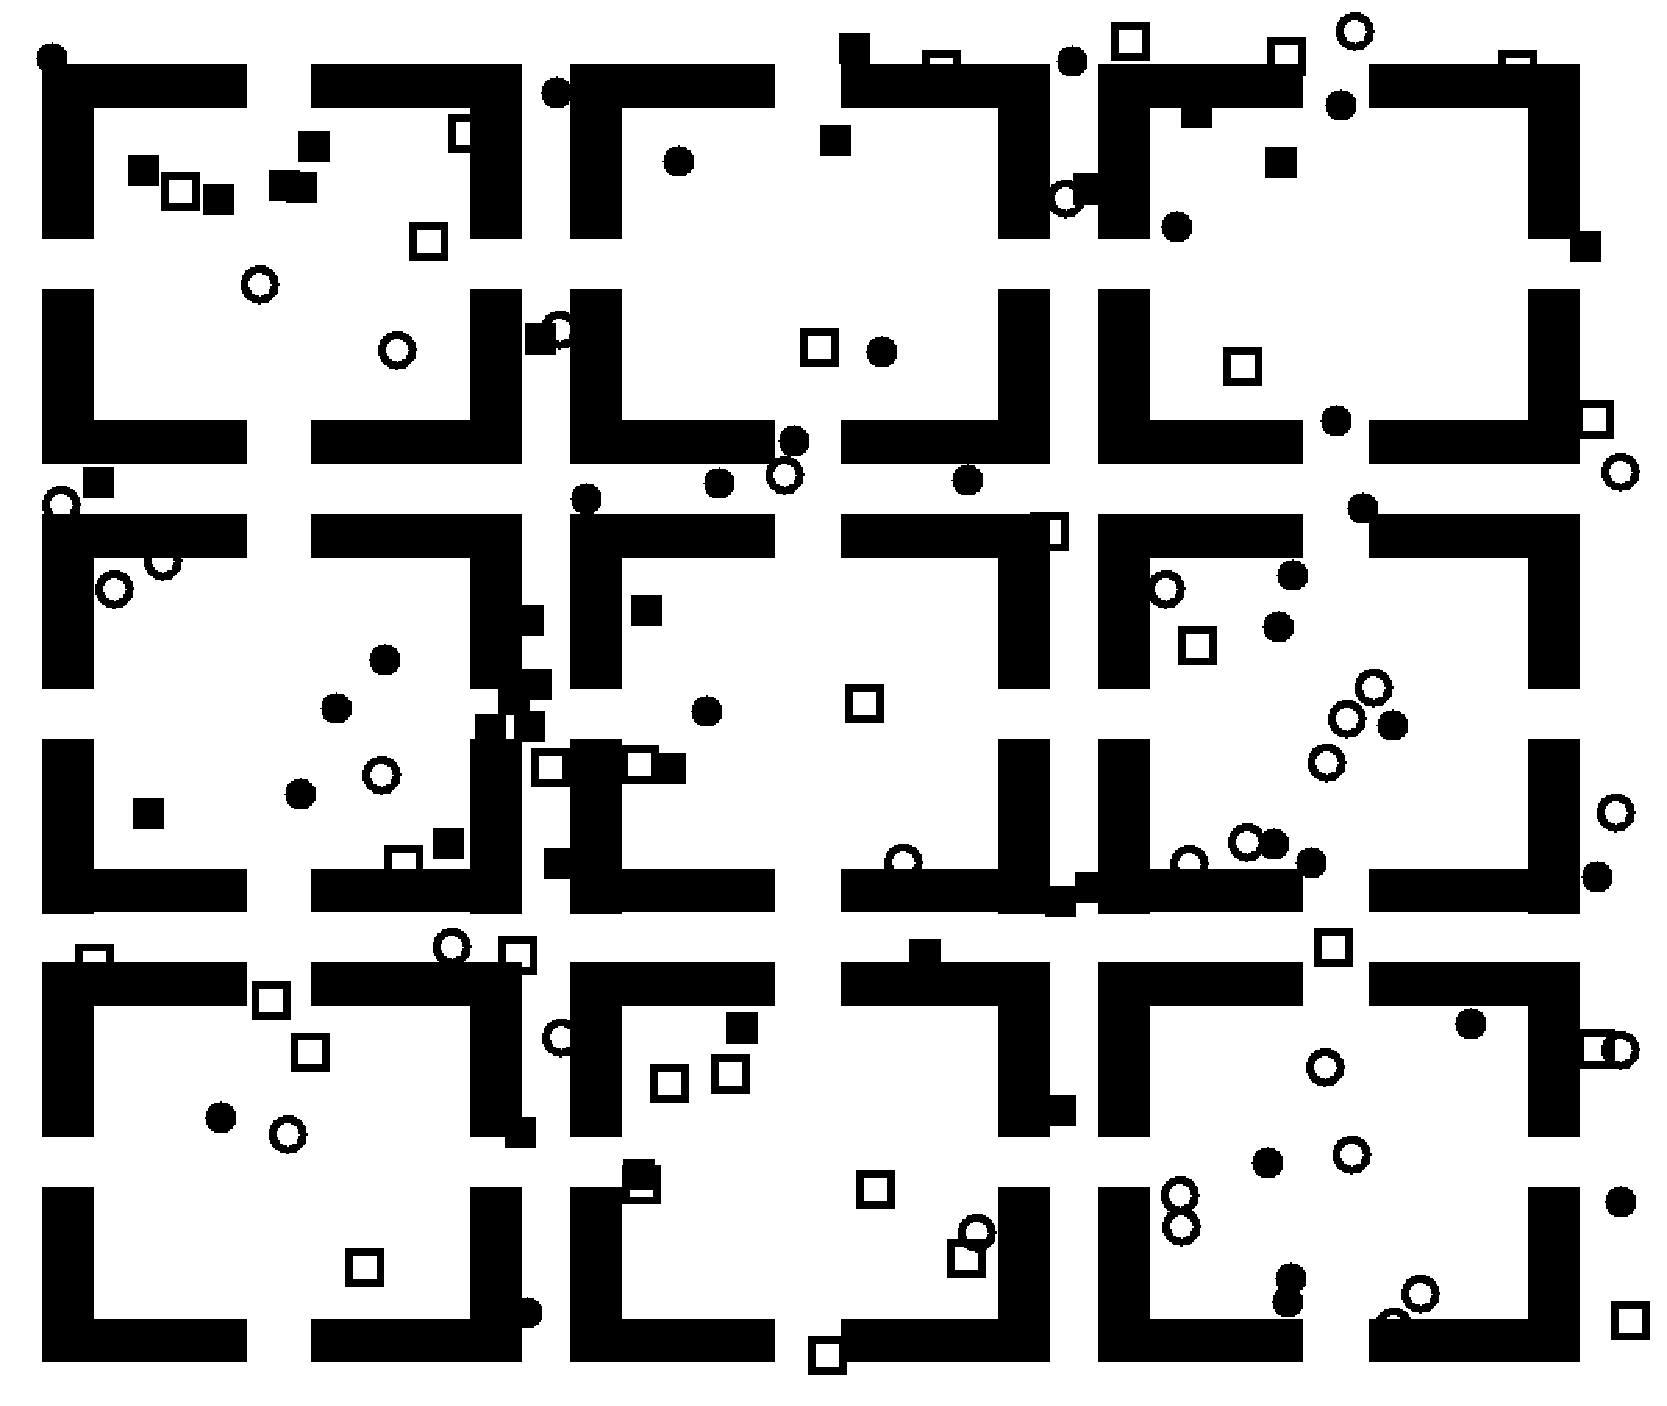
\includegraphics[width=0.3\columnwidth]{img/jos-snapshots/4-1}
    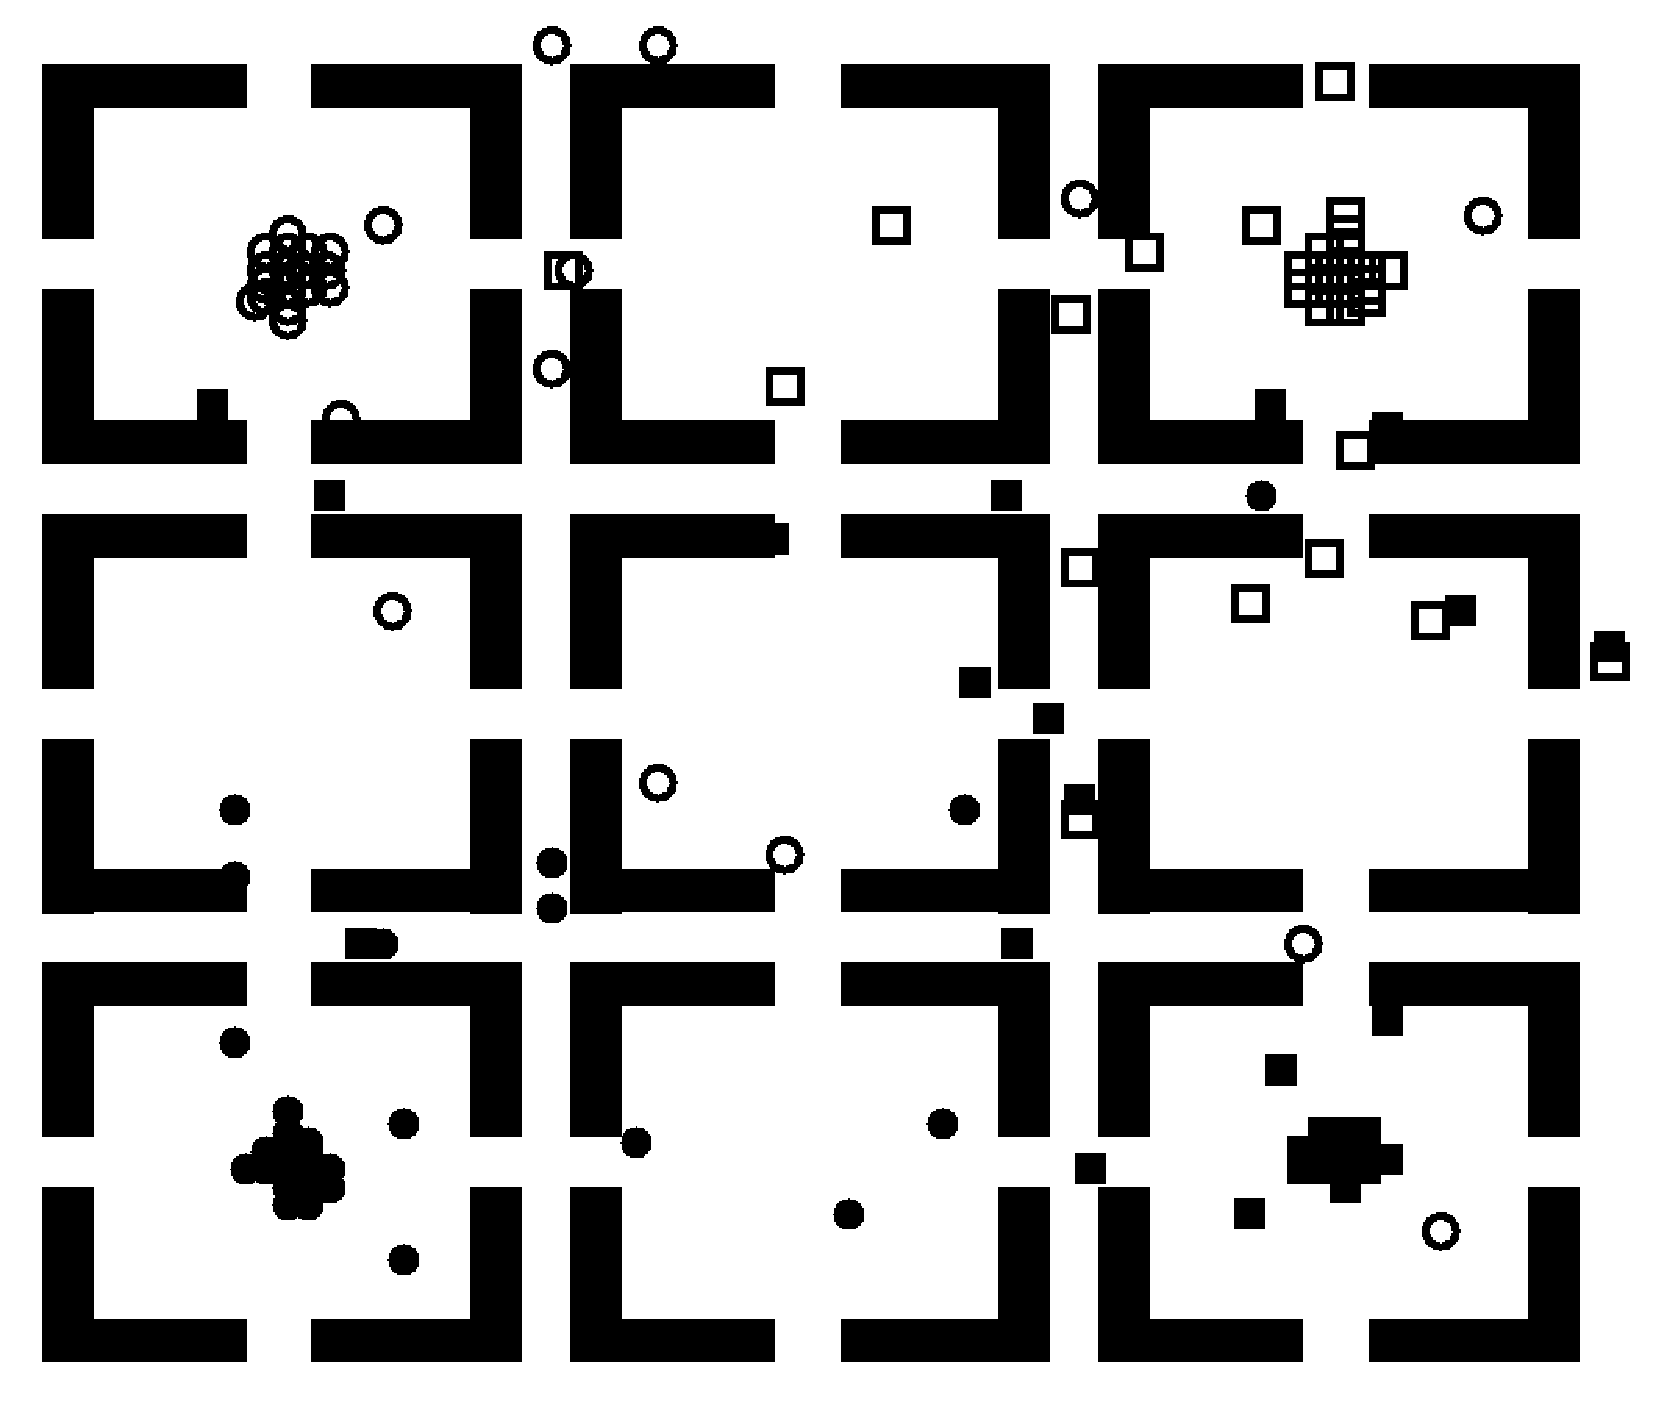
\includegraphics[width=0.3\columnwidth]{img/jos-snapshots/4-3}
    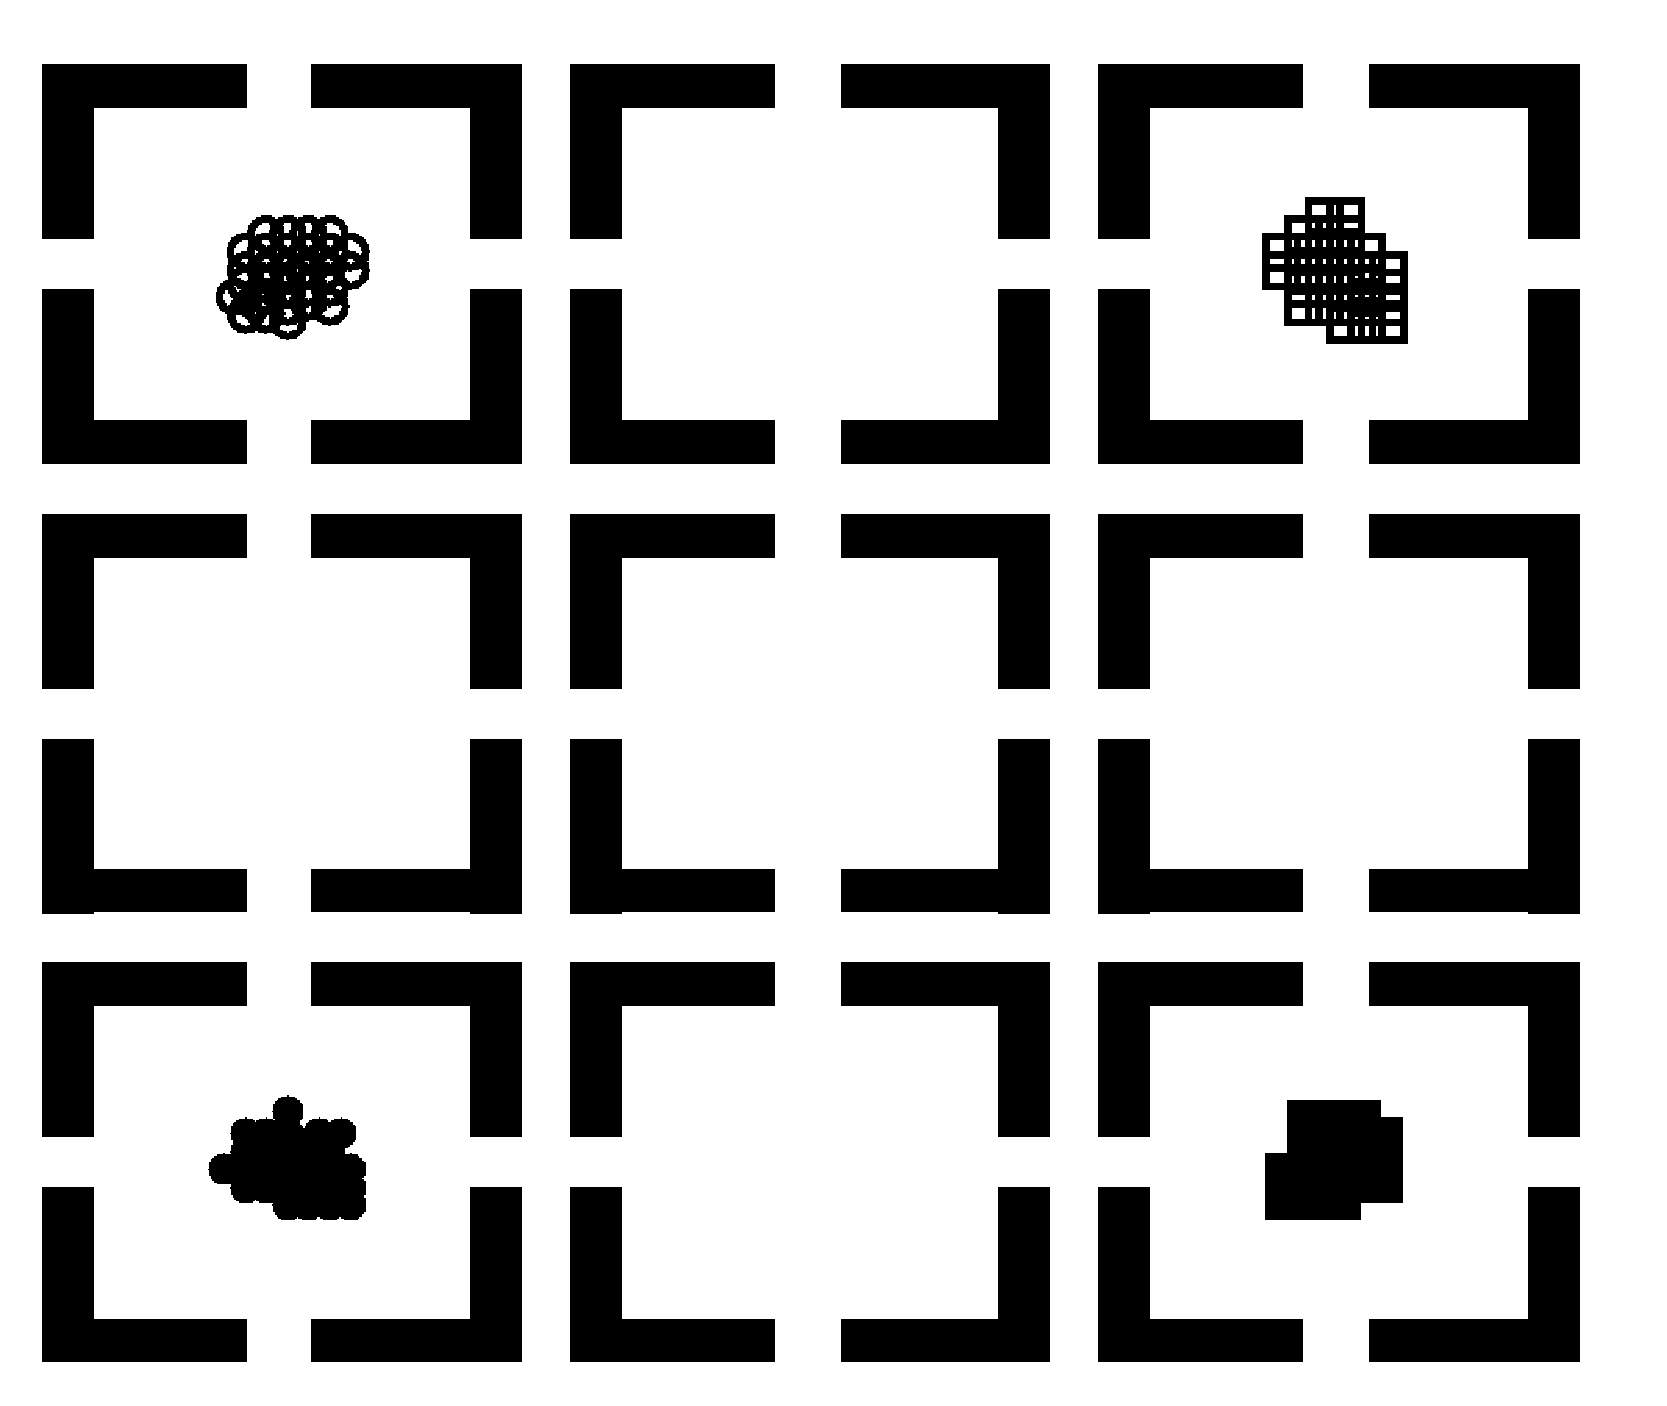
\includegraphics[width=0.3\columnwidth]{img/jos-snapshots/4-4}
    \caption{A simulation run of the reference exposition: three snapshots of \alchemist{}'s graphic reporting module with this simulation. \label{img:museum-generalmap}}    
\end{center}
\end{figure}

We here present simulations conducted over an exposition, where nine rooms are connected via corridors. 
%
People can express different preferences represented by their shape.

Three snapshots of a first simulation run are reported in \Cref{img:museum-generalmap}. 
%
We here consider four different targets that are located in the four rooms near environment angles.
%
People are initially spread randomly in the museum, as shown in the first snapshot, and they eventually reach the room in which the desired target is hosted, as shown in the last snapshot. 


\Cref{img:museum-generalmap2} shows a simulation experimenting with the effect of crowding in the movement of people.
%
Two groups of people -- denoted with empty and full circles -- with common interests are initially located in two different rooms, as shown in the first snapshot. 
%
The target for the dark visitors is located in the central room of the second row, while the others' is in the right room of the second row.
%
In the simulation, dark visitors reach their target soon because it is nearer, thus forming a crowded area intersecting the shortest path towards the target for the other visitors.
%
Due to this jam the latter visitors choose a different path that is longer but less crowded. 

\begin{figure}
\begin{center}
    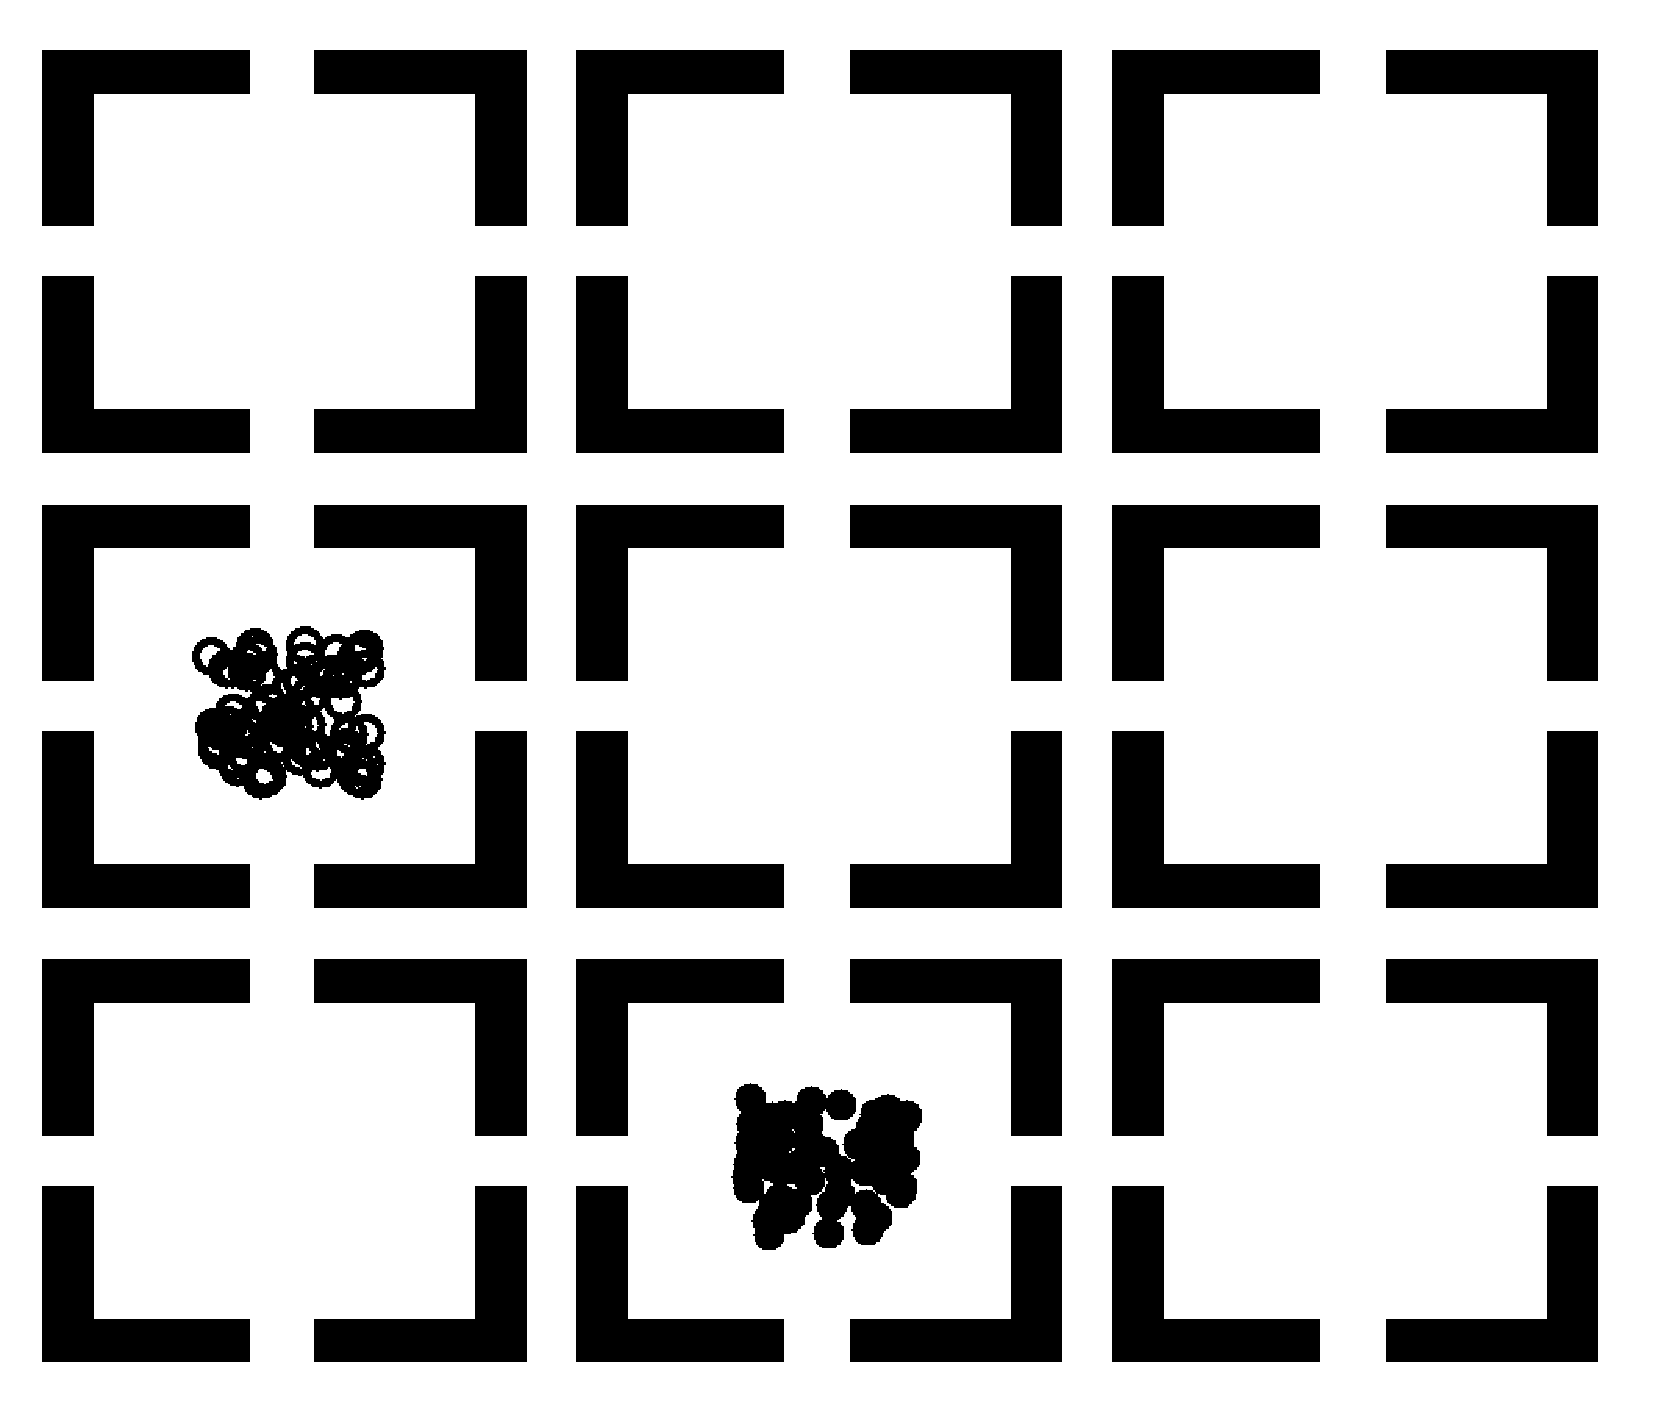
\includegraphics[width=0.3\columnwidth]{img/jos-snapshots/2-1}
    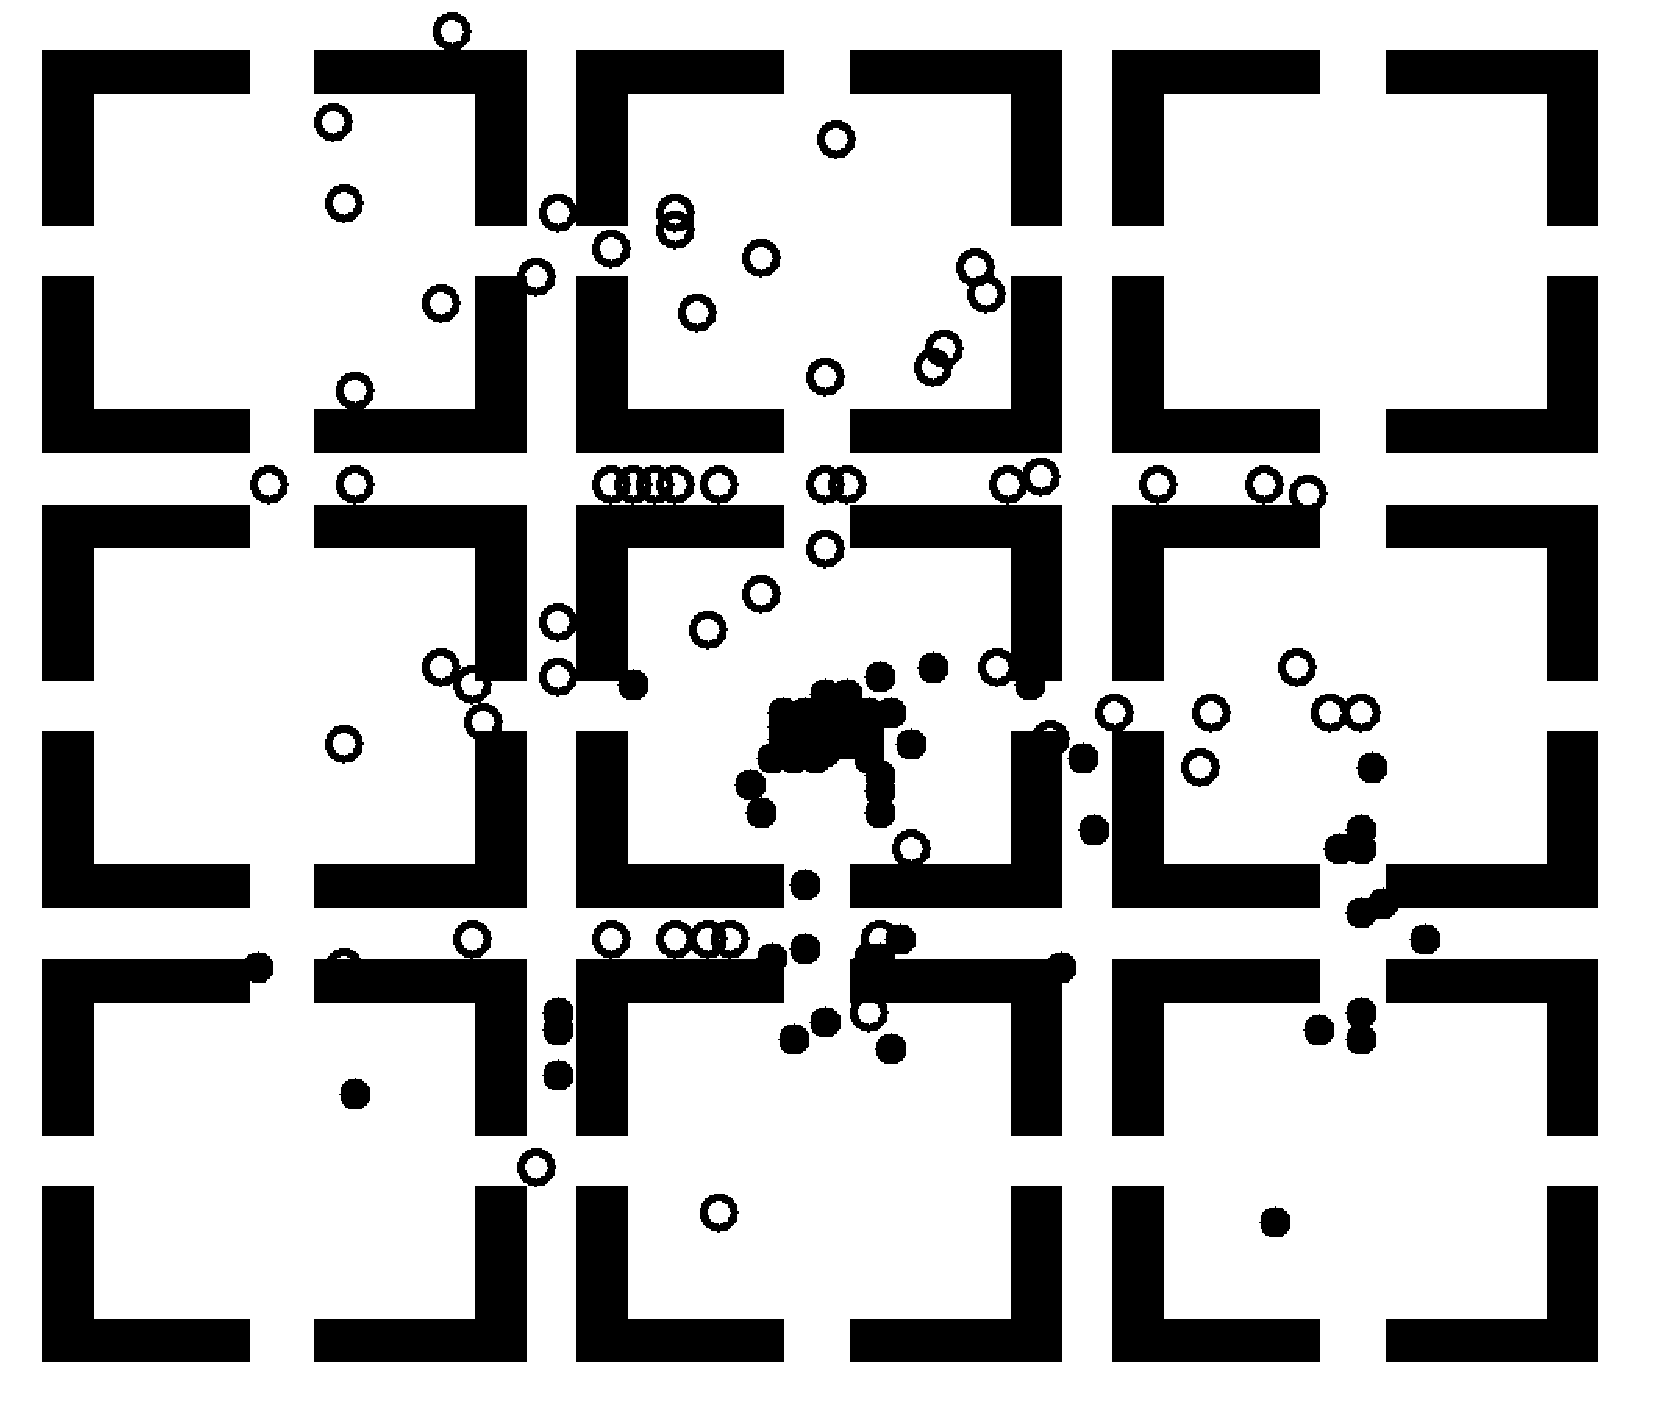
\includegraphics[width=0.3\columnwidth]{img/jos-snapshots/2-3}
    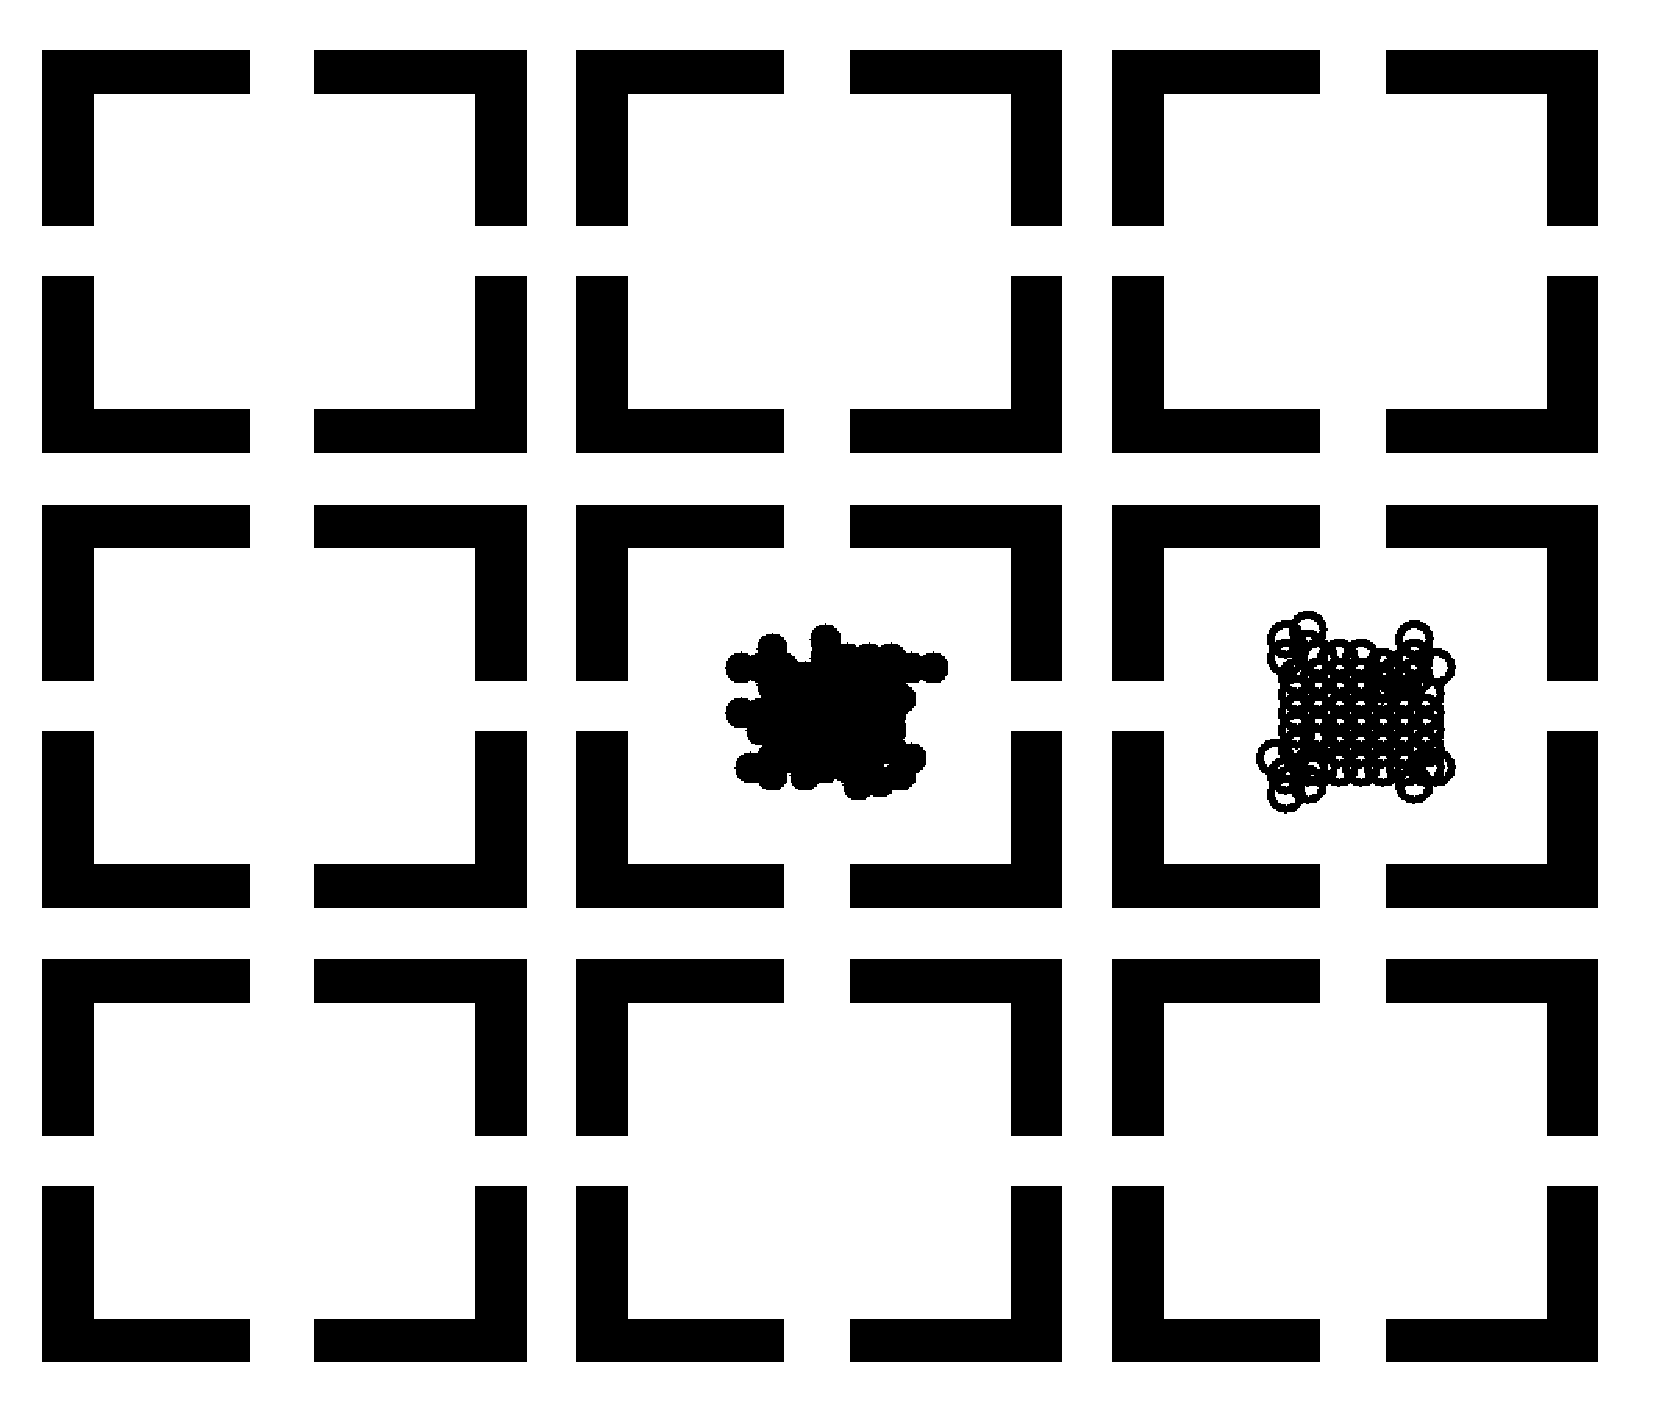
\includegraphics[width=0.3\columnwidth]{img/jos-snapshots/2-4}
    \caption{A run showing the effect of crowding: dark visitors occupy a central room, making other visitors moving left to right by a longer, less crowded path \label{img:museum-generalmap2}}    
\end{center}
\end{figure}

Both tests show qualitative effectiveness of the proposed laws, and suggest that our simulation approach can be used for additional experiments focussing on tuning system parameters (factor $k$) or alternative strategies (e.g., diffusing crowd information) to optimise paths to destinations.
%
For instance, in the context of the second case, \Cref{img:jos-graph} shows how factor $k$ can influence the time for (sub)groups of (light) people to reach the destination, by which we can see that even small values of $k$ lead to a significant improvement---which slowly decreases as $k$ grows.

\begin{figure}
\begin{center}
   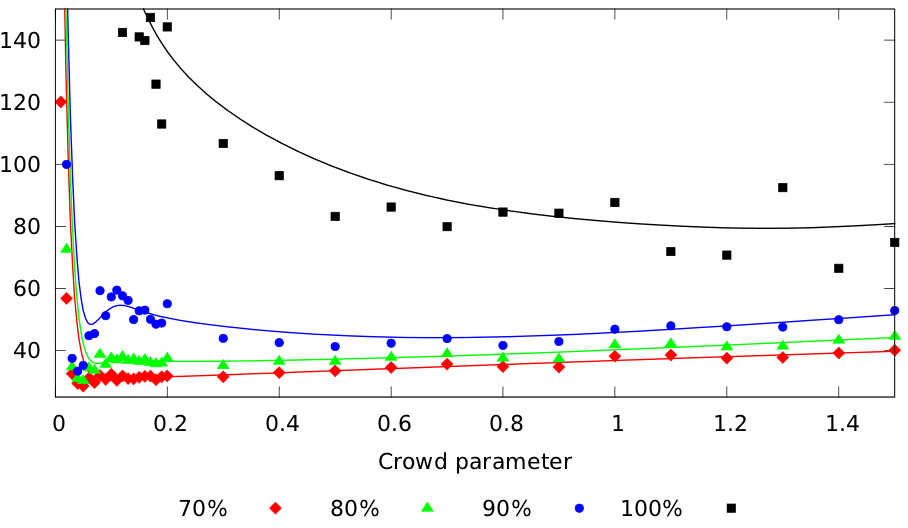
\includegraphics[width=0.99\columnwidth]{img/jos-graph}
   \vspace{-10pt}\caption{Time units of convergence time with different values of crowd parameter and different percentages of people}\label{img:jos-graph}\vspace{-10pt}
\end{center}
\end{figure}


\section{Self composition}
\section{Semantic resource discovery}
\section{Anticipative adaptation}
\label{anticipative-gradient}

\section{Crowd disasters prediction}
\section{Crowd steering at the urban scale}
\label{ahpc-steering}
In section, we focus on the problem of crowd steering at the urban scale.
%
The problem is noticeably different from the classic per-user navigation: we want to consider the current position of people to make the user avoid congested areas, thus reducing the overall trip time and improving the security level.
%
Also, this differs from the experiment in \Cref{jos-museum} for the complexity of the environment and the number of devices involved.
%
Crowds of people vary with time, and consequently we need a system able to dynamically adapt to such changes.
%
As per our line of research, we obviously want the computation to happen in a completely distributed fashion, with no centralised computing system involved.

\subsection{Devices and physical configuration}

We suppose users to be equipped with smart devices, also able to communicate with other devices within a certain range with a wireless technology, and must be able to be aware of their current position.

We also suppose the organisers to have spread around the city some ``static'' network nodes, for instance on public illumination poles, traffic lights, or signals.
%
Such nodes must be equipped with network capabilities similar to those of a Wi-Fi access point.
%
In particular, they must allow nearby mobile devices to connect to all the static nodes within their communication range.
%
There is no upper or lower number or density (devices per square meter) limit to the number of static devices to deploy.
%
The only strict requirement involves both the distance among devices and their communication range: the devices must be placed at a distance and have a communication range large enough such as there is no network segmentation.
%
Besides strict requirements, some other guidelines apply:
\begin{itemize}
 \item it is preferable to displace static nodes in points where there are people, e.g. on streets and crossings;
 \item the wider the number of static nodes that can communicate, the more precise will be the results;
 \item the higher the density of static devices, the more precise will be the results.
\end{itemize}

The last assumption we make is that devices are able to estimate the time needed for walking towards any of the connected device in normal conditions.
%
This last assumption is again perfectly acceptable considering the current technology, where smart devices are always connected to the Internet and can access public navigation services.

\subsection{Distributed crowd steering}

Given the structure described above and the mobile smart devices able to communicate with the static nodes, we now outline a possible software solution.
%
The device wanting to be steered publishes a gradient including the information about the wanted destination.
%
The information about destination can be either expressed as physical location (e.g. latitude and longitude) or as a description: the system works in a fashion totally orthogonal to this choice.
%
One or more static devices located near a potential point of interest (POI) receive such gradient, and react becoming sources of a gradient which measures the distances between nodes.
%
This response gradient diffuses on static nodes until it reaches the source, carrying within itself information about the chain of static devices forming the shortest path.
%
The requester will receive a gradient pointing towards the nearest POI, and can navigate step-by-step by reaching in order all the nodes of the path.
%
Although it is not part of this very experiment, the reply could be tuned to be different depending on the request and on the characteristics of the point of interest.
%
For instance, a value representing the ``level of matching'' between the request and the response could be embedded in the gradient, and used to modify its spatial structure in such a way that POIs more affine with the request are preferred even if farther.
%
Some example of similar usage of gradients is available in \cite{SemMatchingSAC2013}.

Now that a basic form of steering is in place, we can improve it by adding contextual information.
%
We assume that static nodes are able to detect the number of people in their surroundings.
%
Again, this is not critical even in a real deployment, and can be achieved in numerous ways with a different level of precision, which spans from just keeping track of which mobile nodes are connected (and, as a consequence, within the communication range) to the usage of dedicated sensors and techniques (e.g. cameras and computer vision).
%
Let's call $C$ the perceived number of mobile devices surrounding a static node.
%
We can alter the spatial shape of the gradient by acting on the function that outputs the actual distance between devices.
%
For instance, adopting the notation in \Cref{gradient}, we can use $f(n) = \varGamma_{n} +d(n) + K \cdot{} C$ where $K$ is a system parameter.
%
What happens? Basically, areas densely populated with mobile devices will appear as more distant, and consequently the requester will be steered towards alternative routes.
%
The whole system works in a totally emergent and distributed way, with no global knowledge of what's going on, no central control involved, and complete distribution of the computation among its components.

A further refinement of these steering mechanisms involve the ability to react to events that will happen in future (given that there is information about that).
%
The patterns required to do so have already been presented in \Cref{anticipative-gradient}, and the interested reader can deepen reading \cite{anticipativegradient-SASO12}.

\subsection{Simulation in \alchemist{}}
\label{ahpc-simulation}
We decided to focus on the case of mass urban sports events, and in particular on the Vienna City Marathon 2013, an event that every year involves about 40.000 actives and 300.000 spectators.
%
During such event, a smartphone application based on SAPERE \cite{sapere-procedia7} concepts was deployed, and gathered 1503 high quality GPS traces \cite{socinfo2013}.
%
We relied on such data set to build simulations demonstrating our concepts of crowd steering at a urban level.

\begin{figure*}[h]
 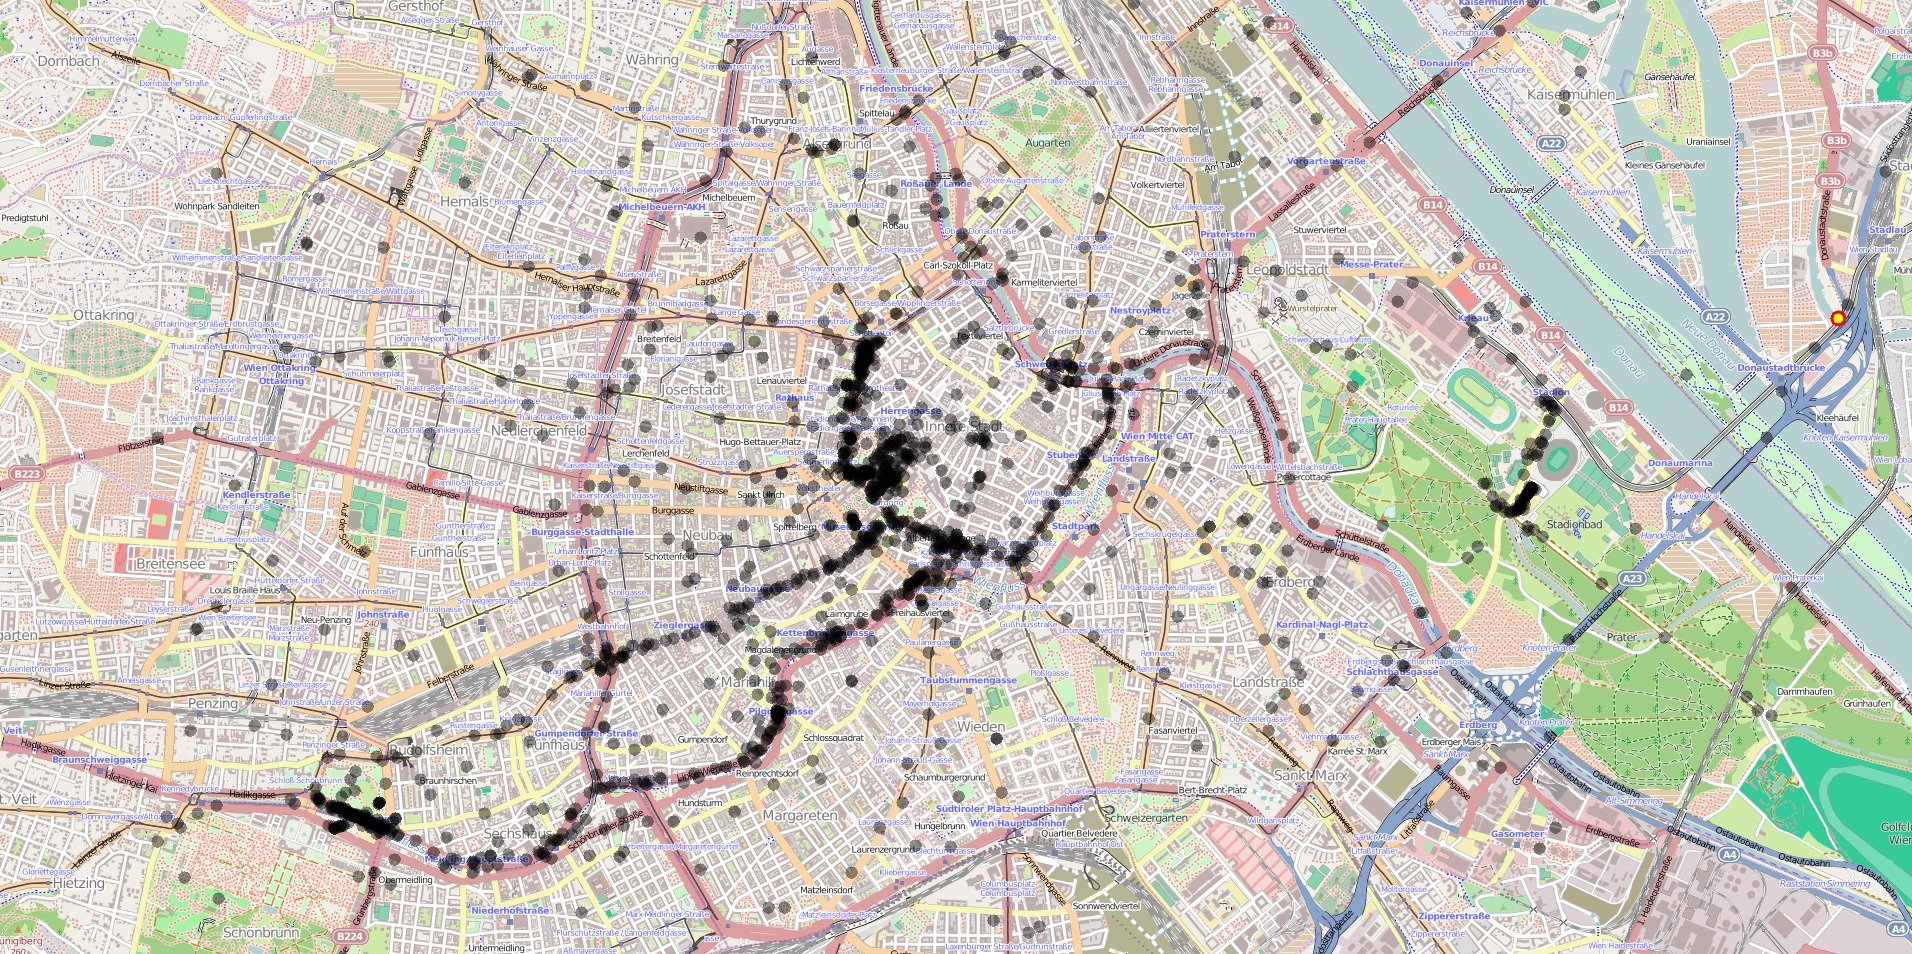
\includegraphics[width=0.99\textwidth]{img/vienna}
  \caption{A snapshot of the whole city of Vienna as simulated in \alchemist{}. This snapshot is taken while simulating the city at 10am, each black point corresponds to a GPS trace. The more an area is crowded, the blacker it appears in the image.}
  \label{img:ahpc-vienna}
\end{figure*}

As \alchemist{} environment, we obviously used the map of Vienna.
%
Another rather straightforward choice was to map each device to a node, supposing the users to carry one and one only device which participates to the system.
%
The network of static nodes was built by creating a grid of 572 devices spread around the city and enabling the positioning in the nearest street point.
%
After that, we positioned a node at Burggarten (48.203926,16.365765), representing our POI, and a node at (48.21441,16.35825) representing our navigation system user.
%
Finally, we positioned the nodes of the users which follow the traces.
%
As result, we had in total 2077 simulated nodes, of which 1504 mobile and moving during the actual simulation, 1503 by following the traces using the mixed mode (see \Cref{img:mixed-alchemist-navi}) and one following the steering system.

As linking rule we decided to let the infrastructure nodes connect to every other node within a communication range of 150 meters. 
%
We used the same set of reactions for each node in the system, but on the mobile nodes, in which also the reactions needed to program the mobility were included.
%
In \Cref{img:ahpc-vienna} a graphical output of the simulator is proposed.
%
We relied on the SAPERE meta-model.
%
This way, we were able to simulate a network of programmable tuple spaces.

\begin{figure}
  \subfigure[Level of crowding in the interested area]{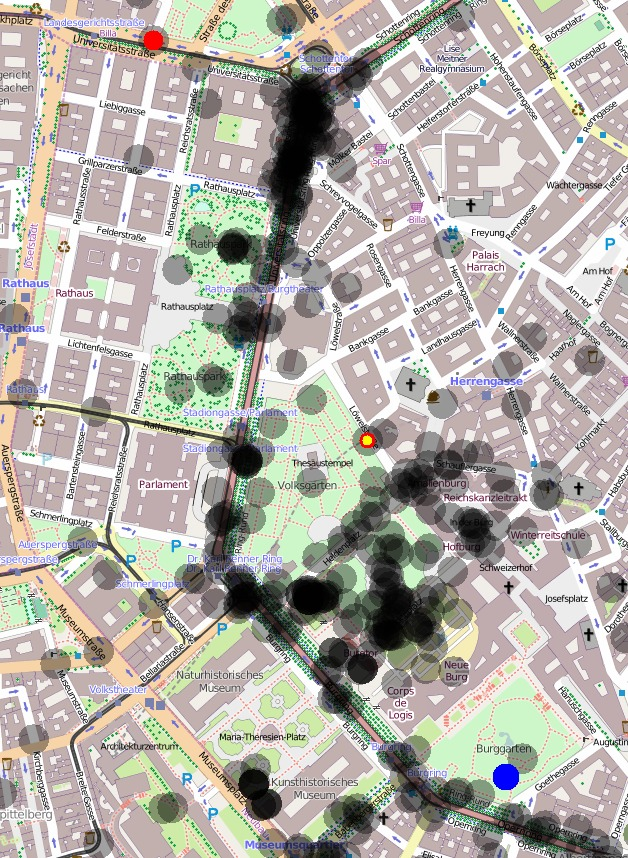
\includegraphics[width=0.315\textwidth]{img/crowd}
   \label{img:ahpc-crowd}
  }
~
  \subfigure[Classic navigation]{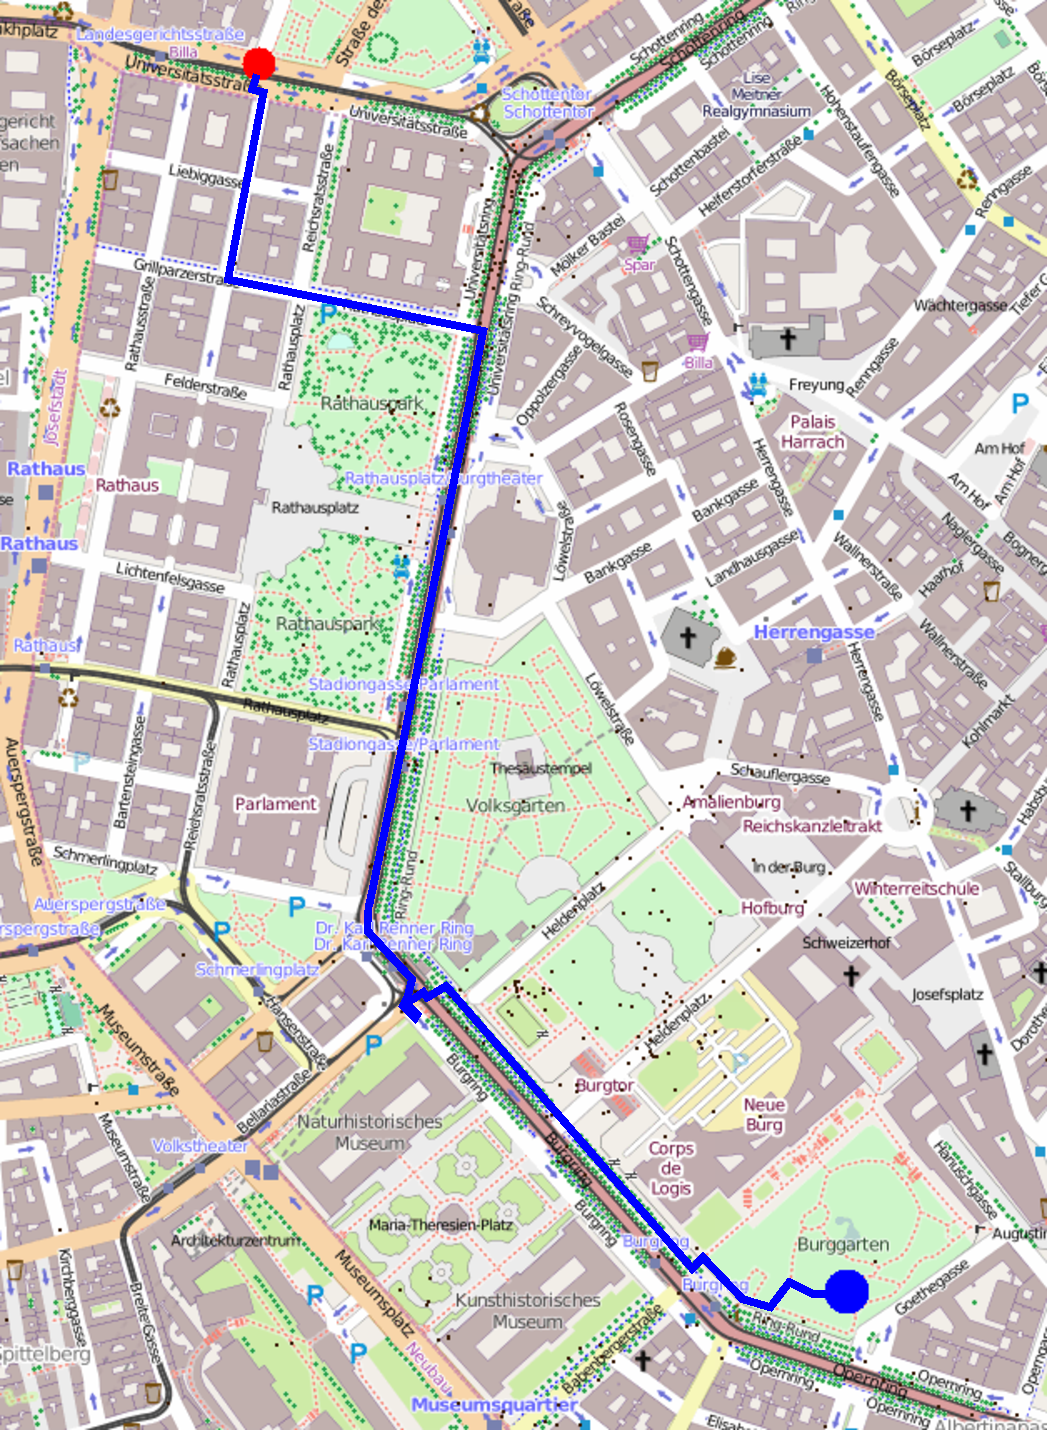
\includegraphics[width=0.315\textwidth]{img/vcm_nocd2}
   \label{img:ahpc-nocrowd}
  }
~
  \subfigure[Crowd-sensitive navigation]{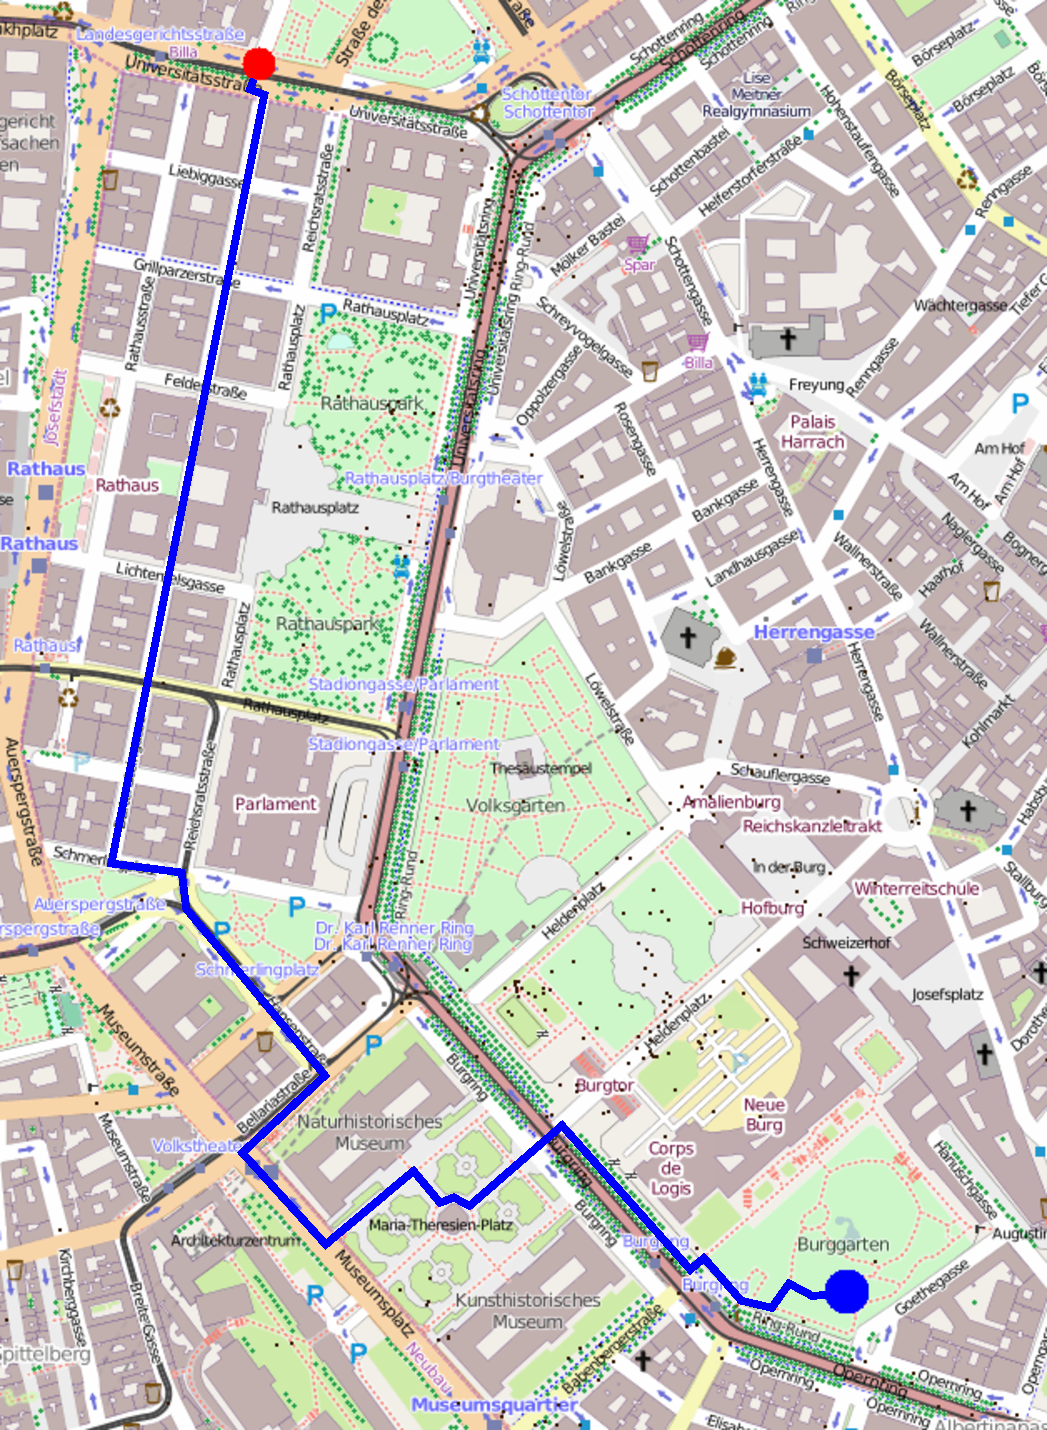
\includegraphics[width=0.315\textwidth]{img/vcm_cd}
   \label{img:ahpc-crowdsteering}
  }
 \caption{In these three snapshots a qualitative evaluation of the crowd-sensitive steering system benefits is offered. The requester is painted in red, while the nearest POI is in blue. In \Cref{img:ahpc-crowd}, the density of people in the area is shown (at the time at which the red node starts): a more intense black mean a more crowded area. In \Cref{img:ahpc-nocrowd} and \Cref{img:ahpc-crowdsteering} is possible to see the suggested routes of, respectively, the classic navigation and the crowd-sensitive navigation. The second suggests a longer but much less jammed path.}
 \label{img:ahpc-steering}
\end{figure}

A complete evaluation of such an emergent environment is all but trivial.
%
The best way to measure the effectiveness of a crowd-sensitive user steering system would probably be the measure of the average walking time on routes generated probabilistically according to the most walked paths.
%
This kind of evaluation has two strong requirements to prove itself scientifically relevant: first, it requires to identify how popular are the routes; second, and most important, it would require a realistic model of pedestrian, including the physical interaction with other people.
%
At the time of writing, we do not have such model, although we are working to find a decent approximation.

As proof of concept, we chose to monitor the path of a single user steered from Universit\"{a}tstrasse to Burggarten.
%
We chose this path because the shortest path connecting the user to her destination includes a walk in between one of the most crowded areas during the sport event, and as such is the perfect test bed for an approach whose goal is to improve the trip time in such conditions.

In \Cref{img:ahpc-steering} a qualitative impact is given.
%
It is immediately clear that the suggested path in \Cref{img:ahpc-crowd} is longer but successfully reduces the space walked within crowded areas, with respect to the one in \Cref{img:ahpc-nocrowd}.

\begin{figure}
 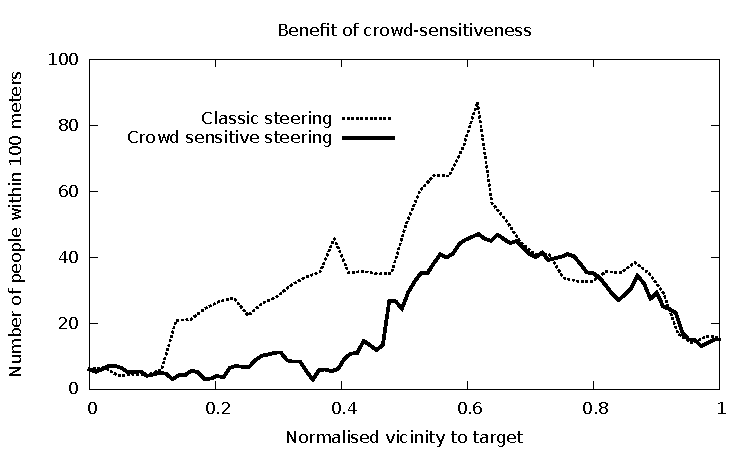
\includegraphics[width=0.99\textwidth]{img/ahpc-chart}
 \caption{This chart shows how the number of users surrounding the user (within 100 meters from her) vary with the proximity to the target.
%
 With ``normalised distance'', we mean that we divided the distance the user still has to walk to reach the target by the total length of the suggested path.
 }
 \label{img:ahpc-chart}
\end{figure}

The chart in \Cref{img:ahpc-chart} confirms the qualitative evaluation.
%
Towards the beginning and the end, the two algorithms have a similar performance, due to the fact that these parts of the walk (as the initial) are common.
%
In the central part of the walk, however, the path suggested by the crowd-sensitive algorithm tends to avoid a considerable amount of jammed areas.
%
We claim that, assuming the traces to be a representative sampling of the actual population of the area and the more crowded areas to be slower to walk (both assumptions sound rather straightforward to the authors), then the crowd sensitive algorithm guarantees an average lower time to destination.

%%%%%%%%%%%%%%%%%%%%%%%%%%%
%%%%%%%%%%%%%%%%%%%%%%%%%%%
%%%%%%%%%%%%%%%%%%%%%%%%%%%
%%%%%%%%%%%%%%%%%%%%%%%%%%%
%%%%%%%%%%%%%%%%%%%%%%%%%%%
%% AGGREGATE PROGRAMMING %%
%%%%%%%%%%%%%%%%%%%%%%%%%%%
%%%%%%%%%%%%%%%%%%%%%%%%%%%
%%%%%%%%%%%%%%%%%%%%%%%%%%%
%%%%%%%%%%%%%%%%%%%%%%%%%%%
%%%%%%%%%%%%%%%%%%%%%%%%%%%
%%%%%%%%%%%%%%%%%%%%%%%%%%%
\chapter{Aggregate programming languages}

When we introduced Field Calculus in \Cref{field-calculus}, we said that it is more a theoretical than a practical framework.
%
Building on the foundation of field calculus, the subsequent step is to provide a framework that can be practically leveraged to express a collection of higher-level ``building block'' algorithms, each a simple and generalized basis element of an ``algebra'' of programs with desirable resilience properties (e.g., the operators presented in~\cite{BV-FOCAS2014}).
%
On top of this, higher-level library APIs can be built, enabling simple and transparent construction of robust distributed systems.

Any practical implementation of field calculus must embed a field calculus interpreter within an architecture that handles the pragmatics of communication, execution, and interfacing with hardware, operating system, and other software.
%
At the same time, it is important that this system be readily portable across both simulation environments and real networked devices.
%
Finally, both system development and maintainability are greatly enhanced if the exact same code is used for execution in all contexts.

Here is where \protelis{} comes into play: it represents our effort to bring Field Calculus to practice, satisfying the requirements stated above.

%TODO: dire che ha anche una parte più teorica, relativa a codice mobile e HOF in field calculus%

\section{Higher order functions in field calculus}
\subsection{Impact on alignment}

\section{\protelis{}: practical aggregate programming}
\label{protelis-language}
We have designed the \protelis{} language as an implementation of the field calculus \cite{VDB-FOCLASA-CIC2013} closely related to Proto~\cite{proto}.
%
On the one hand, it incorporates the main spatial computing features of the field calculus, hence enjoying its universality, consistency, and self-stabilization properties \cite{BVD-SCW14,VD-COORD2014-LNCS2014}.
%
On the other hand, it turns the field calculus into a modern specification language, improving over Proto by providing
\begin{itemize}
 \item access to a richer API through Java integration;
 \item support for code mobility through first-order functions;
 \item a novel syntax inspired by the more widely adopted C-family languages.
\end{itemize}

Protelis is freely available and open source, and can be downloaded as part of the \alchemist{} distribution.

\subsection{Syntax}

We present the \protelis{} language in terms of its abstract syntax, provided in \Cref{img:protelis-syntax} as a means to guide the discussion of the language's features.
%
This syntax uses similar conventions to well-known core languages like Featherweight Java \cite{FJ}.
%
We let meta-variable $\fname$ range over names of user-defined functions, $\var$ over names of variables and function arguments, $\lit$ over literal values (Booleans, numbers, strings), $\oname$ over names of built-in functions and operators (including the ``hood'' functions described in \Cref{protelis-special-operators}), $\mname$ over Java method names, and $\aname$ over aliases of static Java methods.
%
All such meta-variables are used as non-terminal symbols in \Cref{img:protelis-syntax}.
%
Overbar notation $\overline{y}$ generally means a comma-separated list $y_1,\ldots,y_n$ of elements of kind $y$, with the two exceptions that in $\overline{\FCFUNCTION}$ we use no comma separator, and in $\overline{\s}\texttt{;}$ semi-colon is used as separator instead.

\begin{figure}
\centering
\framebox[0.7\textwidth]{$
\begin{array}{l@{\hspace{0.1cm}}c@{\hspace{0.1cm}}l}
     \PROGRAM & \BNFcce & \overline{\tt{I}} \; \overline{\FCFUNCTION} \;
     \overline{\s}; \comment{Program}     \\
     \tt{I} & \BNFcce & \km{\tt{import}} \; \mname \; \BNFmid \;
     \km{\tt{import}} \; \mname \dotK \tt{*} \; % \BNFmid \;
%      \km{\tt{import}} \; \mname \; \km{as} \; \aname \;
     \comment{Java import}\\
       \FCFUNCTION & \BNFcce & \km{\defK} \; \fn{\fname} (\vb{\overline{\var}}) \;\bodyK{\overline{\s};}
     \comment{Function definition}\\
         \s & \BNFcce & \e \; \BNFmid \; 
         \km{\letK} \vb{\var} \km{\asgK} \e \; \BNFmid \;
         \vb{\var} \km{\asgK} \e 
         \comment{Statement}\\
\we & \BNFcce &  \vb{\var}
    \; \BNFmid \; \lit 
    \; \BNFmid \; \tupK{\overline{\we}} 
    \; \BNFmid \; \fname
    \; \BNFmid \; \lambdaK{\overline{\vb{\var}}}{\bodyK{\overline{\s};}}    \comment{Variable/Value} \\
\e & \BNFcce &  \we  \comment{Expression} \\ 
    & \BNFmid & \!\! \oname(\overline{\e})
    \; \BNFmid \; \fn{\fname}(\overline{\e})
    \; \BNFmid \; \e\dotK\km{\applyK}(\overline{\e})\qquad\qquad
    \comment{Fun/Op Calls} \\
    & \BNFmid &  \e\dotK\mname(\overline{\e})
    \; \BNFmid \; \aname(\overline{\e})\qquad\qquad
    \comment{Method Calls} \\ 
   & \BNFmid & \!\! \repK{\vb{\var}}{\we}{\bodyK{\overline{\s};}}
      \comment{Persistent state}  \\
    & \BNFmid & \!\! \ifK{\e}{\bodyK{\overline{\s};}}{\bodyK{\overline{\s}';}}
      \comment{Exclusive branch}  \\
    & \BNFmid & \!\! \muxK{\e}{\bodyK{\overline{\s};}}{\bodyK{\overline{\s}';}}
      \comment{Inclusive branch}  \\
    & \BNFmid & \!\! \nbrK{\bodyK{\overline{\s};}}
      \comment{Neighborhood values}  \\
 \end{array}
 $}
\caption{\protelis{} abstract syntax, colored to emphasize definition and application (red), functions (blue), variables (green), and special field calculus operators (purple).}
\label{img:protelis-syntax}
\end{figure}


\subsection{Ordinary Language Features}

One of the distinctive elements of \protelis{} when compared to other aggregate programming languages (particularly Proto), is the adoption of a familiar C- or Java-like syntax, which can significantly reduce barriers to adoption.
%
Despite this syntactic similarity, \protelis{} is a purely functional language: a program is made of a sequence of function definitions ($\FCFUNCTION_1\ldots\FCFUNCTION_n$), modularly specifying reusable parts of system behavior, followed by a main block of statements.
%
Following the style of C-family languages, a function's body is a sequence of statements surrounded by curly brackets.  As in the Scala programming language\footnote{http://www.scala-lang.org.}, however, statements can also be just expressions, and a statement sequence evaluates to the result of the last statement.
%
Each statement is an expression to be evaluated (\e), possibly in the context of the creation of a new variable ($\km{\letK} \vb{\var} \km{\asgK} \e$) or a re-assignment ($\vb{\var} \km{\asgK} \e$)\footnote{Technically, ``re-assignment'' is actually the creation of a new variable that shadows the old.}.
%
As an example, consider the following function taking four fields as parameters, after the ``channel'' pattern from~\cite{butera}:
\begin{center}
\begin{Verbatim}[samepage=true, frame=single, commandchars=\\\{\}]
\km{def} \fn{channel}(\vb{distA}, \vb{distB}, \vb{distAB}, \vb{width}) \{
   \km{\letK} \vb{d} \km{\asgK} \vb{distA} + \vb{distB};
   \vb{d} \km{\asgK} \vb{d} - \vb{distAB};
   \vb{d} < \vb{width}
\}
\end{Verbatim}
\end{center}
This function assumes that its input \texttt{\vb{distA}} maps each device to its distance to a region $A$, \texttt{\vb{distB}} maps each device to its distance to a region $B$, \texttt{\vb{distAB}} is a constant field holding at each device the minimum distance between regions $A$ and $B$, and \texttt{\vb{width}} is a constant field holding at each device the same positive number.
%
The function then computes a Boolean field, mapping each device to \texttt{true} only if it belongs to a ``channel'' area around the shortest path connecting regions $A$ and $B$ and approximately \texttt{\vb{width}} units wide.
%
All devices elsewhere map to \texttt{false}.

Atomic expressions $\we{}$ can be literal values ($\lit$), variables ($\var$), tuples ($\tupK{\overline{\we}}$), function names ($\fname$) or lambdas ($\lambdaK{\overline{\vb{\var}}}{\bodyK{\overline{\s};}}$).
%
Structured expressions include three kinds of ``calls'': \emph{(i)} $\oname(\overline{\e})$ is application to arguments $\overline{\e}$ of a built-in operation $\oname$, which could be any (infix- or prefix-style) mathematical, logical or purely algorithmic function
%
\footnote{For simplicity of presentation, we omit the syntax for infix operations and order of operations, which is closely patterned after Java.}
%
; \emph{(ii)} $\fn{\fname}(\overline{\e})$ is application of a user-defined function; and \emph{(iii)} $\e\dotK\km{\applyK}(\overline{\e})$ is application of arguments to an expression $\e$ evaluating to a lambda or function name.
%
The following shows examples of such calls:

\begin{Verbatim}[samepage=true, frame=single, commandchars=\\\{\}]
\km{def} \fn{square}(\vb{x}) \{
   \vb{x} * \vb{x};
\}
\km{let} \vb{f} \km{=} \fn{square};
\km{let} \vb{g} \km{=} (\vb{x}) -> \{
   \fn{square}(\vb{x}) + 1
\};
\vb{f}.\km{apply}(\vb{g}.\km{apply}(2))     \il{gives 25 on all devices}
\end{Verbatim}

In addition, arbitrary Java method calls can be imported and used by Protelis: \emph{(i)} $\e\dotK\mname(\overline{\e})$ is method call on object $\e$ and \emph{(ii)} $\aname(\overline{\e})$ is invocation of a static method, via an alias $\aname$ (always starting with '\#') defined by an {\tt import} clause.
%
The alias is created automatically as the bare method name for single imports or imports of all methods in a class with {\tt *}.
%
\protelis{} can thus interact with Java reflection to support dynamic invocation of arbitrary Java code, as shown in the following example:

\begin{Verbatim}[samepage=true, frame=single, commandchars=\\\{\}]
\km{import} \ex{java.lang.Class.forName}
\km{let} \vb{c} \km{=} \ex{#forName}(\str{"String"});
\km{let} \vb{m} \km{=} \vb{c}.\ex{getMethod}(\str{"length"});
\vb{m}.\ex{invoke}(\str{"Lorem ipsum dolor sit amet"})\il{gives 26 on all devices}
\end{Verbatim}

% Note that between {\tt apply} and Java reflection, Protelis offers many of the features of first-class functions.
%
% Critically, however, there are important questions about how to manage aggregate/local relations for distributed first-class functions~\cite{beal2009dynamically}, which are not yet addressed by field calculus.
%
% For this reason, Protelis does not yet offer any neighborhood summary operations applicable to either Java or Protelis functions.

\subsection{Special Field Calculus Operators}
\label{protelis-special-operators}
The remaining constructs of Protelis are the special operations specific to field calculus, dealing with the movement of information across space and time:
\begin{itemize}
	\item Construct $\repK{\vb{\var}}{\we}{\bodyK{\overline{\s};}}$ defines a locally-visible variable $\vb{\var}$ initialized with $\we$ and updated at each computation round with the result of executing body $\bodyK{\overline{\s};}$: it provides a means to define a field evolving over time according to the update policy specified by $\bodyK{\overline{\s};}$.
%
	\item Construct $\nbrK{\bodyK{\overline{\s};}}$ executed in a device gathers a map (actually, a field) from all neighbors (including the device itself) to their latest value from computing $\overline{\s}$. A special set of built-in ``hood'' functions can then be used to summarize such maps back to ordinary expressions.
	%
	For example, {\tt minHood} finds the minimum value in the map.
%
  \item The branching constructs $\muxK{\e}{\bodyK{\overline{\s};}}{\bodyK{\overline{\s}';}}$ and $\ifK{\e}{\bodyK{\overline{\s};}}{\bodyK{\overline{\s}';}}$ perform two critically different forms of branching.
%
	The {\tt mux} construct is an inclusive ``multiplexing'' branch: the two fields obtained by computing $\overline{\s}$ and $\overline{\s}'$ are superimposed, using the former where $\e$ evaluates to \texttt{true}, and the second where $\e$ evaluates to \texttt{false}.
%
	Complementarily, {\tt if} performs an exclusive branch: it partitions the network into two regions: where $\e$ evaluates to \texttt{true} $\overline{\s}$ is computed, and elsewhere $\overline{\s}'$ is computed instead.
\end{itemize}

The following code shows some example uses of these constructs:

\begin{Verbatim}[samepage=true,frame=single, commandchars=\\\{\}]
\km{def} \fn{count}() \{
   \repK{\vb{\var}}{0}{\bodyK{\var + 1\;}}
\}

\km{def} \fn{maxh}(\vb{field}) \{
   maxHood(\nbrK{\{\vb{field}\}})
\}

\km{def} \fn{distanceTo}(\vb{source}) \{
   \fc{rep}(\vb{d} <- Infinity) \{
      \fc{mux} (\vb{source}) \{
         0
      \} \fc{else} \{
         minHood(\fc{nbr}\{\vb{d}\} + nbrRange)
      \}
  \}
\}

\km{def} \fn{distanceToWithObstacle}(\vb{source},\vb{obstacle}) \{
   \fc{if} (\vb{obstacle}) \{
      \fc{Infinity}
   \} \fc{else} \{
      \fn{distanceTo}(\vb{source})
   \}
\}
\end{Verbatim}

Function \texttt{\fn{count}} yields an evolving field, counting how many computation rounds have been executed in each device.
%
Function \texttt{\fn{maxh}} yields a field mapping each device the maximum value of \texttt{\vb{field}} across its neighborhood---note a \nbrK{} construct should always be eventually wrapped inside a ``hood'' function.
%
Function \texttt{\fn{distanceTo}} nests \nbrK{} inside \texttt{\fc{rep}} to create a chain of interactions across many hops in the network, computing minimum distance from any device to the nearest ``source device'' (i.e., where \texttt{\vb{source}} holds \texttt{true}).
%
It does so by a field \texttt{\vb{d}} initially \texttt{Infinity} everywhere, and evolving as follows: \texttt{\vb{d}} is set to $0$ on sources by \texttt{\fc{mux}}, and elsewhere takes the minimum across neighbors of the values obtained by adding to \texttt{\vb{d}} the estimated distance to the current device---a triangle inequality relaxation computing a distance field also often termed \emph{gradient} \cite{original-gradient,crf,VCMZ-TAAS2011}.
%
Finally, function \texttt{\fn{distanceToWithObstacle}} shows exclusive branch at work; \texttt{\fn{distanceTo}(\vb{source})} is computed in the sub-region where there is no obstacle, which causes the computation of distances to implicitly circumvent such obstacles.


\section{Architecture of \protelis{}}
\label{protelis-architecture}
\begin{figure}
\centering
\subfigure[Abstract Architecture]{
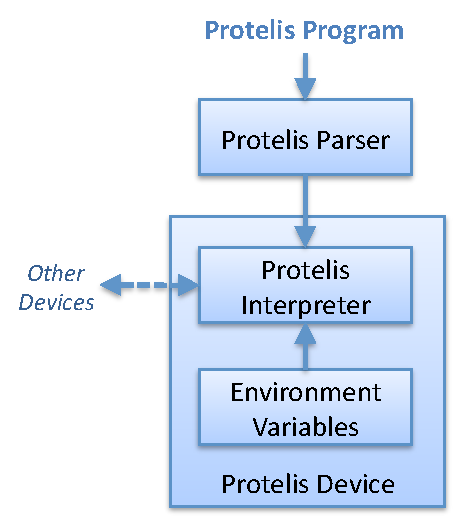
\includegraphics[width=0.4\textwidth]{img/abstract}\hspace{0.05\textwidth}\label{img:protelis-abstract}}
\subfigure[\alchemist{} Simulation]{
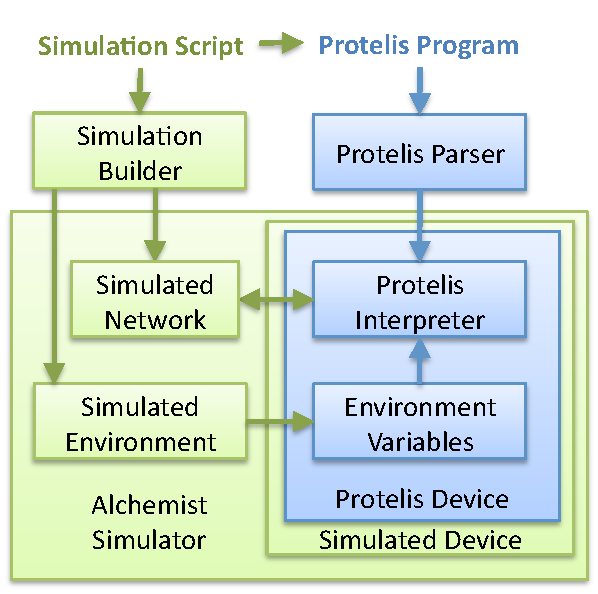
\includegraphics[width=0.5\textwidth]{img/simulated}\label{img:protelis-simulated}}
\subfigure[Network Service Management]{
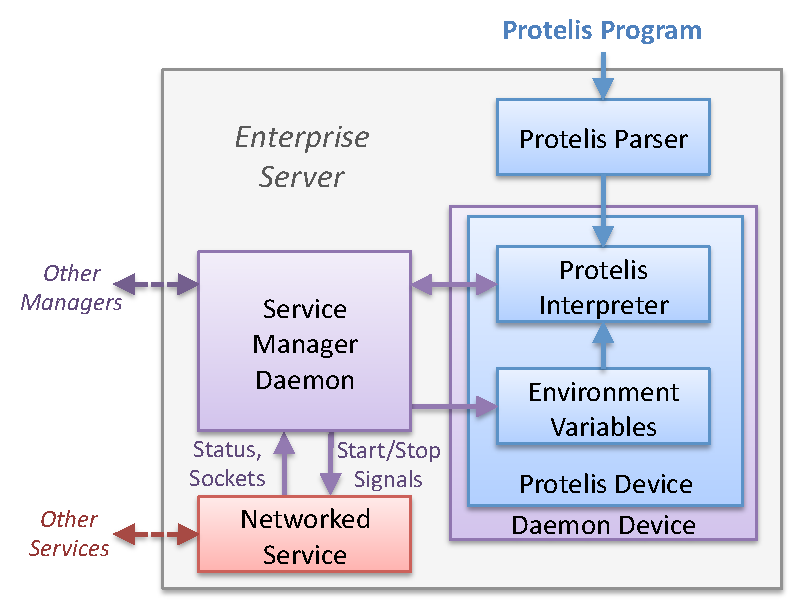
\includegraphics[width=0.6\textwidth]{img/embedded.pdf}\label{img:protelis-embedded}}
\caption{In the abstract Protelis architecture (a), an interpreter executes a pre-parsed Protelis program at regular intervals, communicating with other devices and drawing contextual information from a store of environment variables.
%
This is instantiated by setting when executions occur, how communication is implemented and the contents of the environment.
%
Two such instantiations are presented in this thesis: as a simulation in the \alchemist{} framework (b) and as a daemon for coordinating management of networked services (c).}
\label{img:protelis-architecture}
\end{figure}


In \protelis{}, we designed an architecture, subsumed in \Cref{img:protelis-abstract}, following the same general pattern as was used for the Proto Virtual Machine~\cite{protokernel}.
%
First, a parser translates a text Protelis program into a valid representation of field calculus semantics.
%
This is then executed by a Protelis interpreter at regular intervals, communicating with other devices and drawing contextual information from environment variables implemented as a tuple store of $(token, value)$ pairs.
%
This abstraction is instantiated for use on particular devices or simulations by setting when executions occur, how communication is implemented and the contents of the environment.

We have chosen to implement this architecture in Java.
%
One key reason for this choice is that Java is highly portable across systems and devices.
%
Another key reason (discussed further in the next section) is that Java's reflection mechanisms make it easy to import a large variety of useful libraries and APIs for use in Protelis.
%
Finally, the pragmatics of execution on embedded devices have also changed significantly since the publication of~\cite{protokernel}: a much wider variety of low cost embedded devices are now capable of supporting Java, while at the same time improvements in Java implementations have made it much more competitive in speed and resource cost with low-level languages like C \cite{bull2003, oancea2011}.

In particular, we have chosen to implement Protelis and its architecture via the Xtext language generator~\cite{eysholdt2010xtext} and within the \alchemist{} framework~\cite{alchemist-jos2013}.
%
Usefully, Xtext also features support for generating a language-specific Eclipse plug-in, which provides developer assistance through code highlighting, completion suggestions, and compile-time error detection.

For an initial validation, we have exercised this architecture by construction of two instantiations: one in the \alchemist{} framework for simulation of large-scale spatially-embedded systems; the other as a daemon for coordinating management of networked services.
%
\Cref{img:protelis-simulated} shows the \alchemist{} instantiation: simulations are configured using a simple scripting language, which specifies a Protelis program as well as the collection of devices that will execute it, communication between those devices, and other aspects of the environment to be simulated.
%
The \alchemist{} event-driven simulation engine then handles execution scheduling, message delivery, and updates to the environment tuple store.
%
\Cref{img:protelis-embedded} shows the network service management instantiation.
%
Here, each Protelis device lives on a separate server in an enterprise network, and is tethered to the networked service it is intended to manage by a service manager daemon.
%
This daemon monitors the service, injecting information about its status and known dependencies into the environment and maintaining a neighborhood by opening parallel communication links to the corresponding daemons on any other servers that the monitored service communicates with.
%
Examples using each of these implementations are shown in \Cref{protelis-applications}.

\section{Application examples}
\label{protelis-applications}

To demonstrate how these features combine to offer simple programming of complex distributed algorithms across a potentially broad range of applications domains, we now present two example applications.
%
The first aims at a pervasive computing scenario and is executed in simulation using Alchemist~\cite{alchemist-jos2013}, the second aims at enterprise network management and is executed on a collection of EmuLab~\cite{EmuLab} servers.

\subsection{Rendezvous at a Mass Event}
\label{protelis-rendezvous}

\begin{figure}
\centering
\subfigure[Initial configuration]{
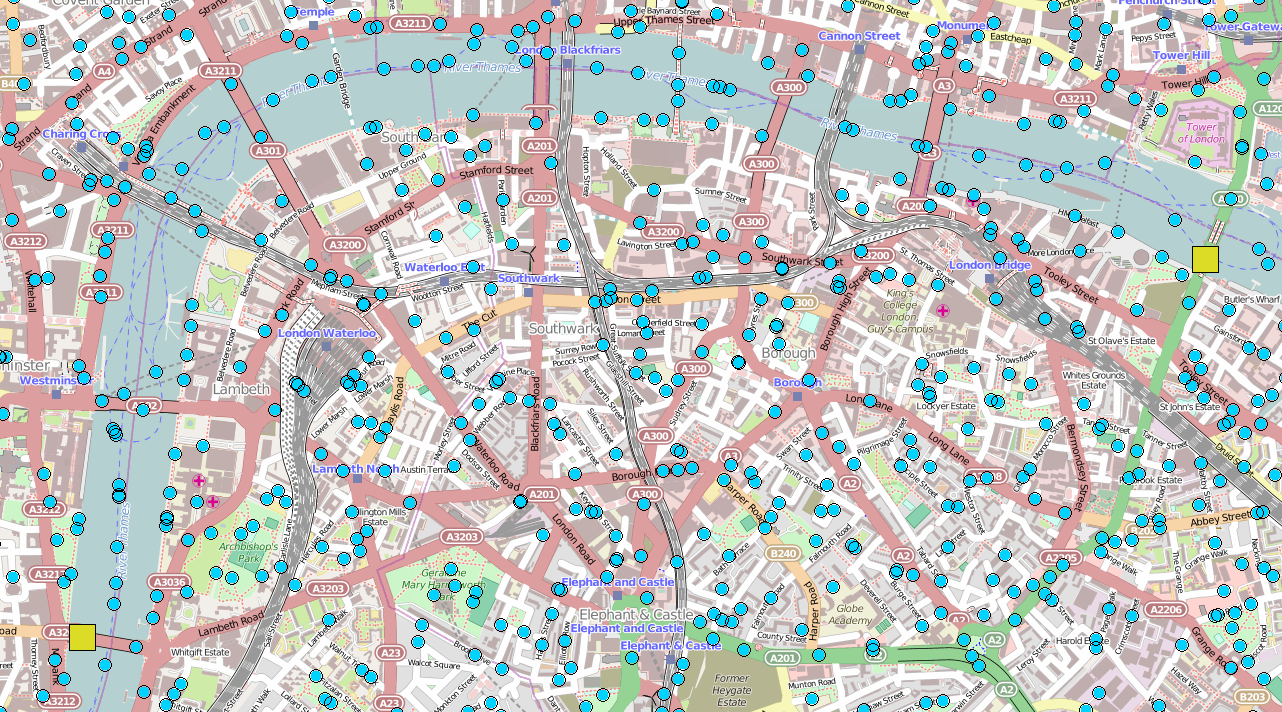
\includegraphics[width=0.48\textwidth]{img/sac15-snapshots/london0}
\label{img:protelis-rendezvous-begin}}
%
\subfigure[Path begins to form]{
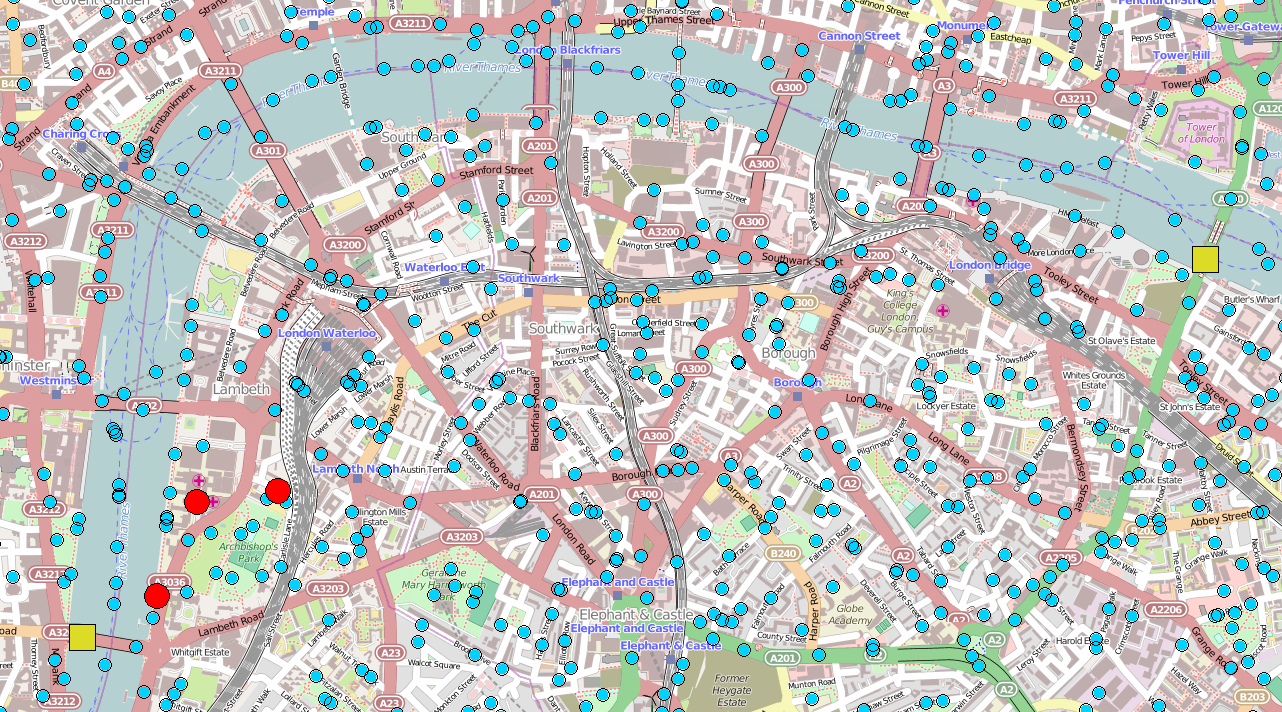
\includegraphics[width=0.48\textwidth]{img/sac15-snapshots/london1}\hspace{0.03\textwidth}
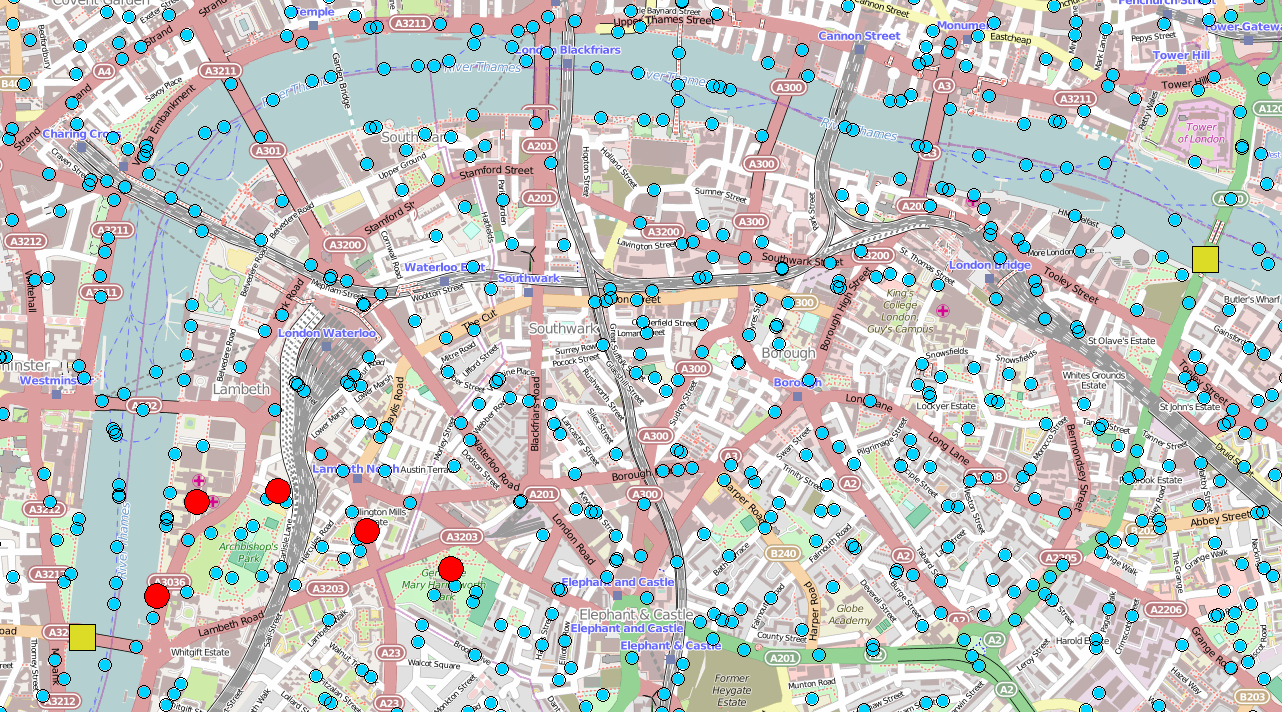
\includegraphics[width=0.48\textwidth]{img/sac15-snapshots/london2}
\label{img:protelis-rendezvous-middle1}}
% 
\subfigure[Path continues to extend]{
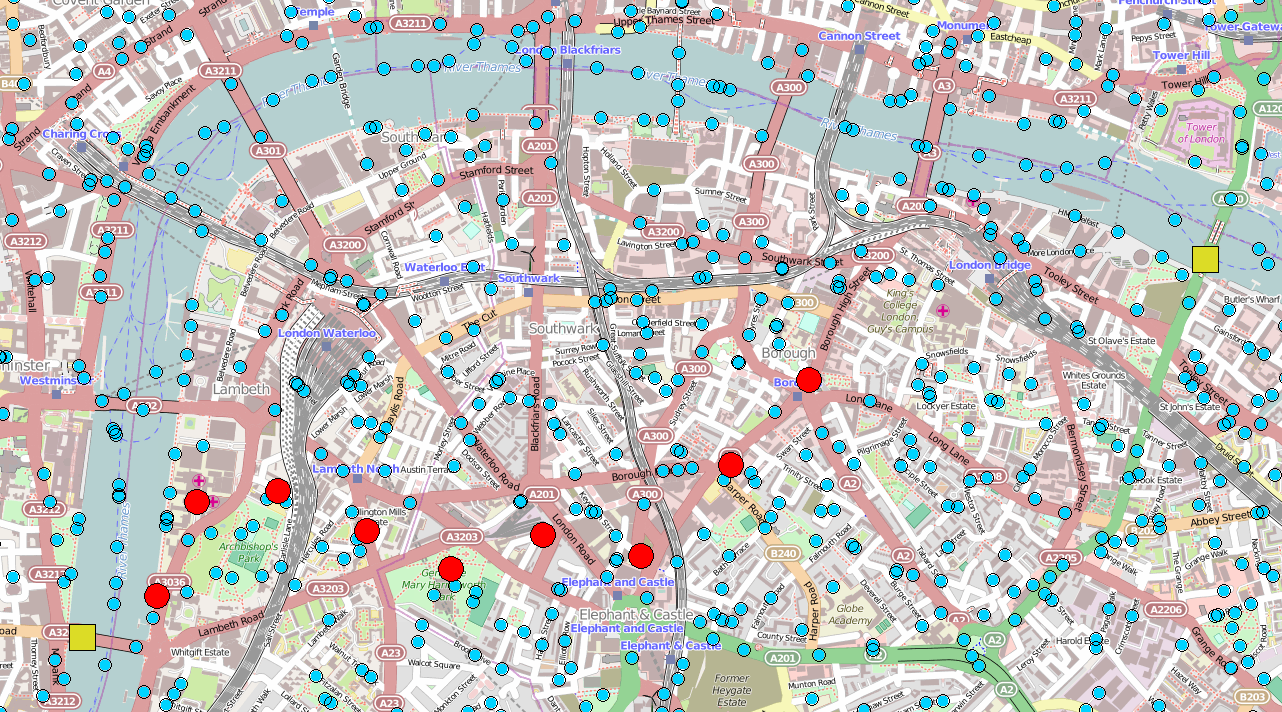
\includegraphics[width=0.48\textwidth]{img/sac15-snapshots/london4}\hspace{0.03\textwidth}
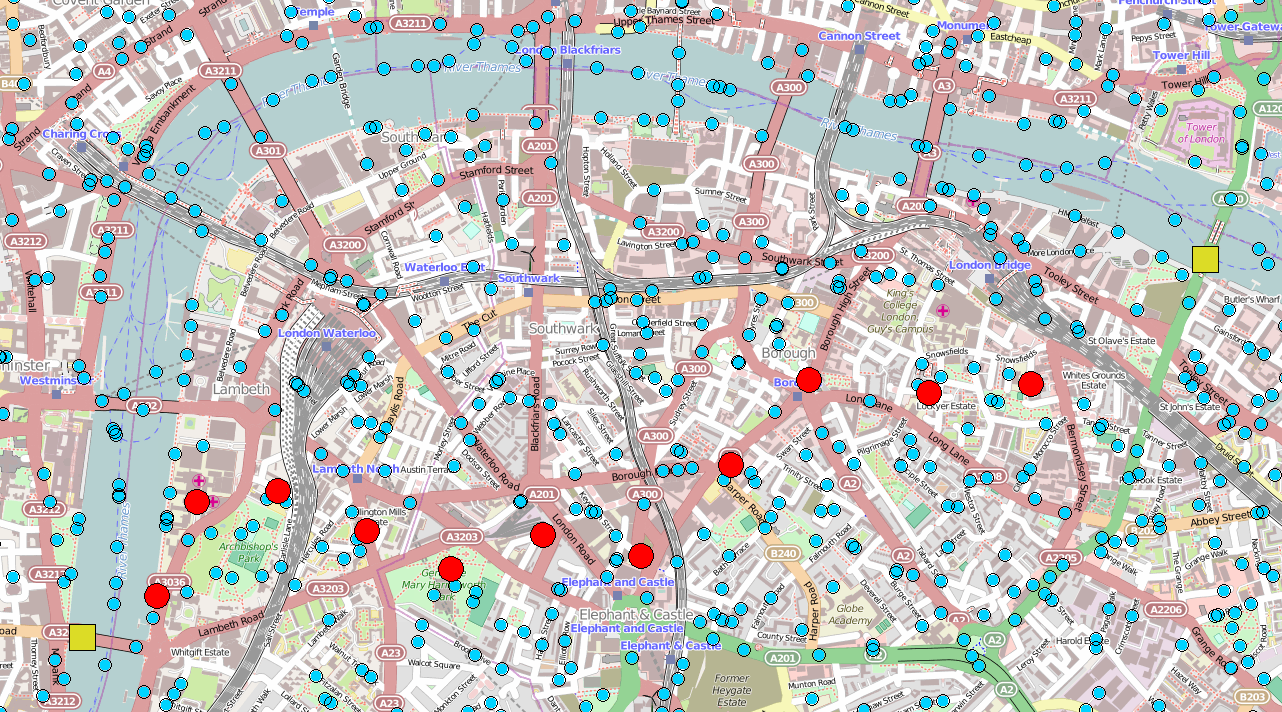
\includegraphics[width=0.48\textwidth]{img/sac15-snapshots/london5}
\label{img:protelis-rendezvous-middle2}}
%
\subfigure[Path computation complete]{
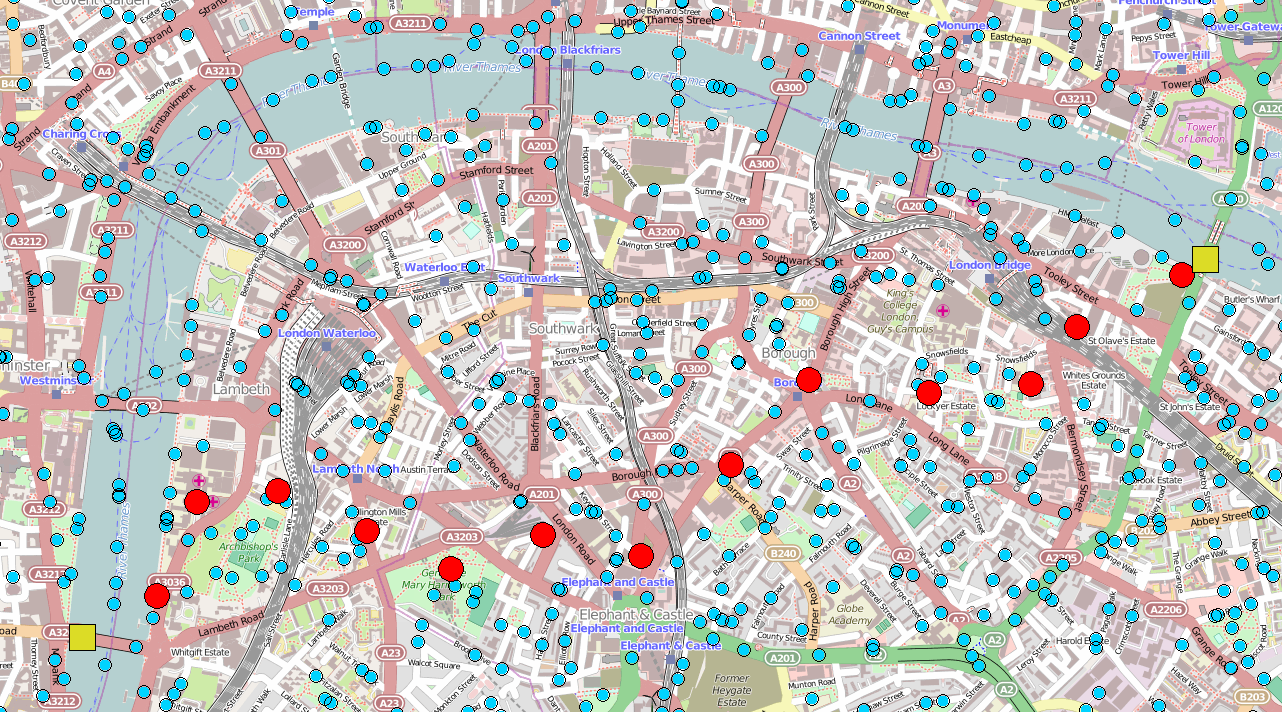
\includegraphics[width=0.48\textwidth]{img/sac15-snapshots/london6}
\label{img:protelis-rendezvous-end}}
% 
\caption{Example of computing a rendezvous route for two people in a crowded urban
environment.}
\label{img:protelis-rendezvous}
\end{figure}

A common problem in large public events is to rendezvous with other companions
attending the same large public event. At mass events, access to external
cloud-based services may be difficult or impossible, and pre-arranged rendezvous
points may be inaccessible or inconveniently distant.
Simple peer-to-peer geometric calculations across the network, however, can
readily compute a route that will allow two people to rendezvous:
% \km{def} \fn{broadcast}(\vb{source},\vb{value}) \{
%   \km{let} \vb{d} \km{=} \fn{distanceTo}(\vb{source});
%   \fc{rep}(\vb{v} <- \vb{value}) \{ \fc{minHood}([\fc{nbr}(\vb{d}),\fc{nbr}(\vb{v})]).get(1) \}
% \}
% \il{Broadcast a value up a distance gradient}
% \km{def} \fn{broadcast}(\vb{source}, \vb{value}) \{
%   \km{let} \vb{d} \km{=} \fn{distanceTo}(\vb{source});
%   \km{let} \vb{lowest} \km{=} \fc{minHood}(\fc{nbr}(\vb{d}));
%   \fc{rep}(\vb{v} <- \vb{value}) \{
%      \fc{mux} (\vb{source}) \{
%        \vb{value}
%      \} \fc{else} \{
%        \fc{minHood}(\fc{mux}(\fc{nbr}(\vb{d})==\vb{lowest})\{ \fc{nbr(v)} \}\fc{else}\{ Infinity \}) 
%      \}
%   \}
% \}
\begin{Verbatim}[samepage=true, frame=single, commandchars=\\\{\}]
\il{Follow the gradient of a potential field down from a source}
\km{def} \fn{descend}(\vb{source},\vb{potential}) \{
   \fc{rep}(\vb{path} <- \vb{source}) \{
      \km{let} \vb{nextStep} \km{=} \fc{minHood}(\fc{nbr}([\vb{potential}, \fc{self}.\ex{getId}()]));
      \fc{if} (\vb{nextStep}.\ex{size}() > 1) \{
         \km{let} \vb{candidates} = \fc{nbr}([\vb{nextStep}.\ex{get}(1), \vb{path}]);
         \vb{source} || \fc{anyHood}([\fc{self}.\ex{getId}(), true] == \vb{candidates})
      \} \fc{else} \{
         \vb{source}
      \}
   \}
\}
\km{def} \fn{rendezvous}(\vb{person1}, \vb{person2}) \{
   \fn{descend} (\vb{person1} == \vb{owner}, \fn{distanceTo}(\vb{person2} == \vb{owner}))
\}
\il{Example of using rendezvous}
\fn{rendezvous}(\str{"Alice"}, \str{"Bob"});
\end{Verbatim}

\Cref{img:protelis-rendezvous} shows an example of running this rendezvous process in a simulated city center.
%
We chose London as a simulation environment, using Alchemist's capability for importing OpenStreetMap data.
%
We displaced 1000 devices randomly across the city streets (represented by pale blue dots), with a communication range of 475 meters (this range chosen to ensure no network segmentation).
%
We then picked two devices whose owners want to meet: one device on Lambeth Bridge (lower left of the image) and one device on Tower Bridge (upper right), each marked with a yellow square.
%
To mark the devices for Protelis, we injected their environments with a property \texttt{\vb{owner}}, assigning the strings \texttt{"Alice"} and \texttt{"Bob"} as values for the first and the second device respectively.

% gradient = 6
% descend = 11
% rendezvous = 3
% expresson = 1
% Total = 21
Implementing this application requires only 21 lines of code: the listing above and the function \texttt{\fn{distanceTo}} that can be found in \Cref{protelis-special-operators}.
%
This implementation measures distance to one of the participants, creating a potential field, then, starting from the other one, builds an optimal path descending the distance potential field to return to the first participant at distance zero.
%
The first half of the algorithm has already been described, and relies on \texttt{\fn{distanceTo}}, while the second half is implemented by the function \texttt{\fn{descend}}.
%
This function, given a device and a potential field, builds a path of devices connecting the former with the source of the latter.
%
The strategy is to mark the device we want to connect to the potential field's source as part of the path, and then, in every device, compute which of the neighbors is closest to the destination.
%
Given this information, a device is in the path if one of the neighbors is in the path already and has marked this device as the closest of its neighbors towards the destination.
%
Note how the whole algorithm can be elegantly compressed into just a few lines of code, and how there is no need to explicitly declare any communication protocol for exchanging the required information, thanks to the repeated use of the $\nbrK$ operator.

As \Cref{img:protelis-rendezvous} shows, once the simulation starts, a chain of devices is rapidly identified (red dots), marking a sequence of way-points for both device owners to walk in order to meet in the middle.
%
Note also that, due to the ongoing nature of the computation, if one of the device owners moves in a different direction instead, the path will automatically adjust so that it continues to recommend the best path for rendezvous.

\subsection{Example: Network Service Management}

One of the common problems in managing complex enterprise services is that there are often many dependencies between different servers and services.
%
Frequently, some of these services are legacy or poorly coded, such that they do not respond gracefully to the failure of their dependencies.  These services may continue to attempt to operate for some time, creating inconsistent state, or may be unable to resume service correctly after the server they depend on is brought back on line.

Thus, responding to a service failure often requires a coordinated shutdown and restart of services in an order dictated by service dependencies.
%
This type of service management can be automated by attaching a daemon that watches the state of each service, then communicates with the daemons of other services to coordinate shutdown and restart in accordance with their dependencies.

\begin{figure}[t!]
\centering
\subfigure[Example Dependent Services Scenario]{
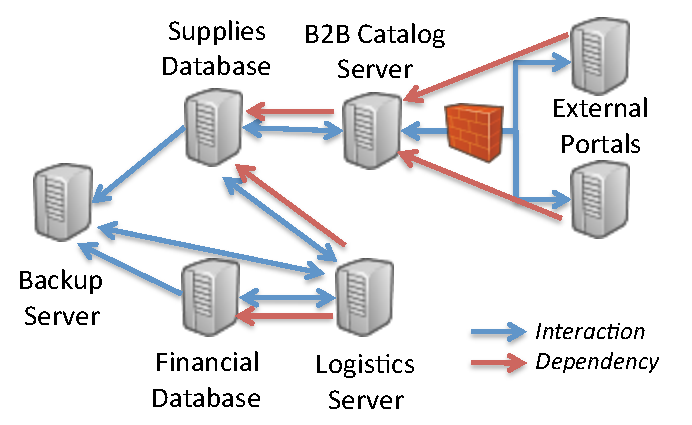
\includegraphics[width=0.8\textwidth]{img/managementScenario}\label{f:restartScenario}}
\subfigure[Example of Coordinated Restart Execution]{
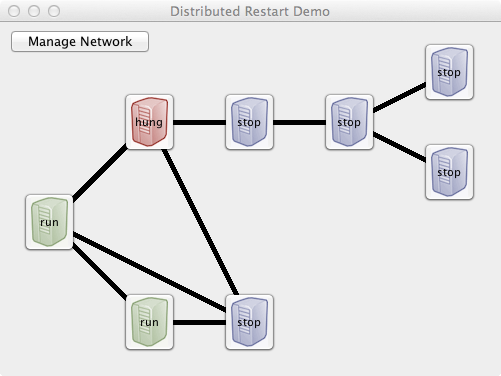
\includegraphics[width=0.8\textwidth]{img/management}\label{f:restartExecution}}
\caption{(a) An example scenario of an enterprise network for a small
manufacturing and supply company. (b) Example of execution on a network of 8
EmuLab~\cite{EmuLab} machines: the supplies database has crashed (red), and so
all dependent services have shut themselves down (blue), while other services
continue to run normally (green).}
\label{f:restart}
\end{figure}

\Cref{f:restartScenario} shows an example scenario of an enterprise network for a small manufacturing and supply company, with dependencies between two key databases and the internal and external servers running web applications.
%
This scenario was implemented on a network of EmuLab~\cite{EmuLab} servers.
%
The services were emulated as simple query-response networking programs in Java that entered a ``hung'' state either upon being externally triggered to crash or after their queries began to consistently fail. 

Each service was wrapped with an embedded Protelis execution engine, which was interfaced with the services by a small piece of monitoring glue code that inserted environment variables containing an identifier for the {\tt serviceID} running on that server, a tuple of identifiers for {\tt dependencies}, and the current {\tt managedServiceStatus} of {\tt stop}, {\tt starting}, {\tt run}, {\tt stopping}, or {\tt hung}.
%
The glue code also provides {\tt stopService} and {\tt startService} methods to send signals to the service, tracks interactions between the services in order to maintain the set of neighbors for Protelis, and allows an external monitoring application to attach and receive status reports.

Dependency-directed coordination of service starting and stopping was then implemented as follows:
%
\begin{Verbatim}[samepage=true, frame=single, commandchars=\\\{\}]
\km{import} \ex{it.unibo.alchemist.language.protelis.datatype.Tuple.*}
\km{import} \ex{com.bbn.a3.distributedrestart.DaemonNode.*}

\il{Compare required and available services}
\km{let} \vb{nbr_set} \km{=} \fc{unionHood}(\fc{nbr}([\ex{serviceID}]));
\km{let} \vb{nbr_missing} \km{=} \ex{dependencies}.\ex{subtract}(\vb{nbr_set});
\km{let} \vb{nbr_required} \km{=} \ex{#contains}(\ex{dependencies},\fc{nbr}(\ex{serviceID})); 
\km{let} \vb{nbr_down} \km{=} \fc{nbr}(\ex{managedServiceStatus}==\str{"hung"} ||
                   \ex{managedServiceStatus}==\str{"stop"});

\il{Is service currently safe to run?}
\km{let} \vb{problem} \km{=} \fc{anyHood}(\vb{nbr_down} && \vb{nbr_required}) ||
            !\vb{nbr_missing}.\ex{isEmpty}();

\il{Take managed service up and down accordingly}
\fc{if} (\ex{managedServiceStatus}==\str{"run"} && \vb{problem}) \{
  \ex{#stopProcess}(\ex{managedService});
\} \fc{else} \{
  \fc{if} (\ex{managedServiceStatus}==\str{"stop"} && !\vb{problem}) \{
    \ex{#startProcess}(\ex{managedService});
  \} \fc{else} \{
    \ex{managedServiceStatus}
  \}
\}
\end{Verbatim}
In this program, each device shares information about its service ID and status with its neighbors, enabling them to track which dependencies are currently down or missing.
%
When there is a problem with dependencies, the device invokes {\tt stopProcess} to shut its service down, when dependencies are good, it brings it up again with {\tt startProcess}, and when it is hung it waits for a human to sort out the problem.

\Cref{f:restartExecution} shows a typical screenshot of the network of services in operation on an EmuLab network of Ubuntu machines, one service per machine, as visualized by the monitoring application.
%
In this screenshot, the supplies database has crashed, causing many of the other services to gracefully shut themselves down.  As soon as the supplies database is restarted, however, the rest of the services automatically bring themselves up in dependency order.

\part{Conclusion}
\chapter{Results achieved}

\section{Integrated toolchain for pervasive ecosystems}

\section{Aggregate programming languages}

%TODO: fixme

\subsection{Higher Order Functions in Field Calculus}

\subsection{\protelis{}}
Protelis ensures universality and coherence between aggregate specification and local execution by building atop the field calculus introduced in \cite{VDB-FOCLASA-CIC2013}.
%
At the same time, accessibility, portability, and ease of integration are ensured by embedding Protelis within Java.
%
This enables Protelis programs to draw on the full breadth of available Java APIs and to readily integrate with a wide range of devices and applications, as illustrated by our examples of pervasive computing simulation and networked service management.
%
This implementation of Protelis thus forms an important component of the toolchain necessary for practical application of aggregate programming principles and methods to address real-world problems.
%

\chapter{Future and ongoing work}

%TODO fixme
The \protelis{} framework continues to be actively developed:
%
we plan to enrich it in the future by adding higher-level abstractions
for aggregate programming grounded on the mechanisms discussed in this
work.


\section{Biochemical meta model for \alchemist{}}
ciao

%\appendix
%\input{appendix-a.tex}
%\input{appendix-b.tex}
%\input{appendix-c.tex}

%\input{publication.tex}

%===============================================================================
\small\protect\newpage\addcontentsline{toc}{chapter}{Bibliography}
\bibliography{thesis}
\bibliographystyle{alpha}
%===============================================================================

%\listoffigures
%\listoftables

\end{document}
